\documentclass[a4paper,11pt]{book}
\usepackage[T1]{fontenc}
\usepackage{lmodern}
\usepackage[english]{babel}

% \documentclass{article}
\usepackage[utf8]{inputenc}
\title{Finance and capital markets}
\author{Matteo Romiti}
\date{\today}
\usepackage{natbib}
\usepackage{xcolor}
\usepackage{url}
\usepackage{pagecolor,lipsum}% http://ctan.org/pkg/{pagecolor,lipsum}
\usepackage[]{graphicx}
\usepackage{amsmath}
\usepackage{color}   %May be necessary if you want to color links
\usepackage{hyperref}
\hypersetup{
    colorlinks=true, %set true if you want colored links
    linktoc=all,     %set to all if you want both sections and subsections linked
    linkcolor=blue,  %choose some color if you want links to stand out
}


%%%%%%%%%%%%%%%%%%%%%%%%%%%%%%%%%%%%%%%%%%%%%%%%%%%%%%%%%%%%%%%%%%%%%%%%%%%%%%%%
% 'dedication' environment: To add a dedication paragraph at the start of book %
% Source: http://www.tug.org/pipermail/texhax/2010-June/015184.html            %
%%%%%%%%%%%%%%%%%%%%%%%%%%%%%%%%%%%%%%%%%%%%%%%%%%%%%%%%%%%%%%%%%%%%%%%%%%%%%%%%
\newenvironment{dedication}
{
   \cleardoublepage
   \thispagestyle{empty}
   \vspace*{\stretch{1}}
   \hfill\begin{minipage}[t]{0.66\textwidth}
   \raggedright
}
{
   \end{minipage}
   \vspace*{\stretch{3}}
   \clearpage
}

%%%%%%%%%%%%%%%%%%%%%%%%%%%%%%%%%%%%%%%%%%%%%%%%
% Chapter quote at the start of chapter        %
% Source: http://tex.stackexchange.com/a/53380 %
%%%%%%%%%%%%%%%%%%%%%%%%%%%%%%%%%%%%%%%%%%%%%%%%
\makeatletter
\renewcommand{\@chapapp}{}% Not necessary...
\newenvironment{chapquote}[2][2em]
  {\setlength{\@tempdima}{#1}%
   \def\chapquote@author{#2}%
   \parshape 1 \@tempdima \dimexpr\textwidth-2\@tempdima\relax%
   \itshape}
  {\par\normalfont\hfill--\ \chapquote@author\hspace*{\@tempdima}\par\bigskip}
\makeatother

%%%%%%%%%%%%%%%%%%%%%%%%%%%%%%%%%%%%%%%%%%%%%%%%%%%
% First page of book which contains 'stuff' like: %
%  - Book title, subtitle                         %
%  - Book author name                             %
%%%%%%%%%%%%%%%%%%%%%%%%%%%%%%%%%%%%%%%%%%%%%%%%%%%

% Book's title and subtitle
\title{\Huge \textbf{Finance and Capital Markets}\\}
% Author
\author{\textsc{Matteo Romiti}\thanks{\url{https://matteoromiti.github.io/}}}


\begin{document}
% \pagecolor{yellow!30!orange}
\frontmatter
\maketitle

\begin{dedication}
To all the curious people out there.
\end{dedication}

\hypertarget{ToC}{}
\tableofcontents

\mainmatter

\chapter*{Preface}
This document has been conceived as a way to explain and keep track of what I learned while taking the "Finance and Capital Markets" course publicly available at \url{https://www.khanacademy.org/economics-finance-domain/core-finance}. Notes, thoughts and images come from and are inspired by video lessons and comments posted on the course website. This material may contain errors and misunderstandings. The reader is invited to help me in improving this work.

\section*{Acknowledgements}
My deepest gratitude to Salman Amin Khan.

\chapter{INTEREST AND DEBT}
\begin{chapquote}{Aaron Swartz}
``Be curious. Read widely. Try new things. What people call intelligence just boils down to curiosity.''
\end{chapquote}

\section{Forms of interest}
\subsection{Compound and simple interest}
If you deposit a total sum of money $S$ to a bank with a compound annual interest of $r$\footnote{I'll always assume risk-free interest rates, if not specified.} (e.g., $r=0.1=10\%$) and you wait $n$ years, then your new total sum will be:

\begin{equation}\label{eq:annual_compound_interest}
S' = S(1+r)^n .
\end{equation}

In case of simple annual interest, after $T$ years you would have:

\begin{equation}\label{eq:annual_simple_interest}
S' = S\big(1+rT\big) .
\end{equation}

From equation~\ref{eq:annual_compound_interest} we can compute the number of years $n$ needed to increase our initial sum $S$ of a factor $\beta$:

\begin{equation}\label{eq:time_to_double}
n = \dfrac{\ln{\beta}}{\ln{1+r}}.
\end{equation}

\subsection{The rule of 72}
An approximation to quickly evaluate the time needed to double our money is "the rule of 72". Assume again we have a compound annual interest $r$, then we have to wait $\dfrac{72}{100r}$ years. If the compound interest is a monthly interest, then it would be $\dfrac{72}{100r}$ months. Simple example: with a compound annual interest of $r=9\%$ we should wait 8 years.

\subsection{Continuous compounding interest}
If I lend you a sum $S$ for one year with an interest rate $r$, then at the end of the year you owe me $S'=S(r+1)$. But let's suppose that you may be able to give me the money back in a half a year. In this case, I'd reasonably half the interest at $r'=r/2$, hence you'll give me $S'=S(r'+1)$, but if you miss the payment, then I'll lend you $S'$ at the same interest for another half year, so you'll pay me $S''=S(r'+1)^2$.
If you want to try to set a monthly deadline instead of a semestral one, than it'd be:

\begin{equation}\label{eq:tmp}
S'=S\bigg(1+\dfrac{r}{12}\bigg)^{12}.
\end{equation}

You could also consider days or hours instead of months. If $r=1$ and the interval is infinitesimal, you'll get $S'=eS$, where $e$ is the Euler's number. More generally, if I lend you money for $T$ years and we compound $n$ times per year then it'd be:

\begin{equation}\label{eq:tmp_general}
S'=S\bigg(1+\dfrac{r}{n}\bigg)^{nT}.
\end{equation}

Using the previous limit to get $e$ we can compute the formula for continuous compounding interest:

\begin{equation}\label{eq:continuous_compounding_interest}
S'=Se^{nT}.
\end{equation}

\section{Time value of money}
\subsection{Discounting}
If I have now an amount $S$ of money, then $S$ is the present value. If I have the option of a compound annual interest rate $r$, then the future value $S'$ in $n$ years would be the one obtained in equation~\ref{eq:annual_compound_interest}. So if I'm told that someone is willing to give me $S'$ in $n$ years, I can compute the present value $S$ simply as:

\begin{equation}\label{eq:annual_discount_interest}
S = \dfrac{S'}{(1+r)^n} .
\end{equation}

This is known as discounting. If the interest rate decreases the present value of $S'$ will increase. Discount rates can change depending on the time the money is lent for. The longer the period, the higher the rate.

The annual percentage rate ($APR$) can be obtained from compounding the daily percentage rate ($DPR$):

\begin{equation}\label{eq:APR}
APR = 365 \cdot DPR .
\end{equation}

Alternatively, the money $S'$ owed at day $d$ would be:

\begin{equation}\label{eq:DPR}
S' = S (1+DPR)^d.
\end{equation}

Due to decimal number precision, the result of equation~\ref{eq:DPR}, which is the effective $APR$ may differ from $S\cdot APR$.

\section{Additional notes}

\subsection{Risk-free and risk premium}
Think of an interest rate as the cost of money, which just like the cost of production, labor, and other expenses is a factor of a company's profitability.

The fundamental cost of money to an investor is the Treasury note rate, whose return is guaranteed by the "full faith and credit" of the U.S. government. According to financial theory, a stock's value proposition starts there: stocks are risky assets, even riskier than bonds because bondholders are paid their capital before stockholders in the event of bankruptcy. Therefore, investors require a higher return for taking on extra risk by investing in stocks instead of Treasury notes, which are guaranteed to pay a certain return.

The extra return that investors can theoretically expect from stocks is referred to as the "risk premium." Historically, the risk premium runs at around five percent. This means that if the risk-free rate (the Treasury note rate) is four percent, then investors would demand a return of nine percent from a stock. Therefore, the total return on a stock is the sum of two parts: the risk-free rate and the risk premium.

\subsection{Required rate of return}
The required rate of return is the minimum return an investor expects to achieve by investing in a project. An investor typically sets the required rate of return by adding a risk premium to the interest percentage that could be gained by investing excess funds in a risk-free investment.

There is an inverse relationship between required return and the price investors assign to a stock. Why? Let's say people in the market are looking for a way to make \$10 from investing and they all decide to buy stock A because it has a price of \$100 and will give exactly a ROC of 10\% after one year. Let's say that after one year people want to invest again, but this time the company is expected to perform better and have a ROC of 20\%. If people are still looking for an income of \$10, they will buy stock A for \$50. In this case, higher return means lower price (with fixed income). If instead there is more money to be invested and more people is investing, they will be willing to pay higher prices for the same income, which means lower returns. 

If interest rates are high, the cost of money will be high. This means that for a company to borrow money will be more difficult and it will have to work harder and generate higher returns. High interest rates normally prevent people from buying things and companies from investing in growth opportunities. As a result, sales and profits drop, as do share prices.

% \begin{figure}
%     \centering
%     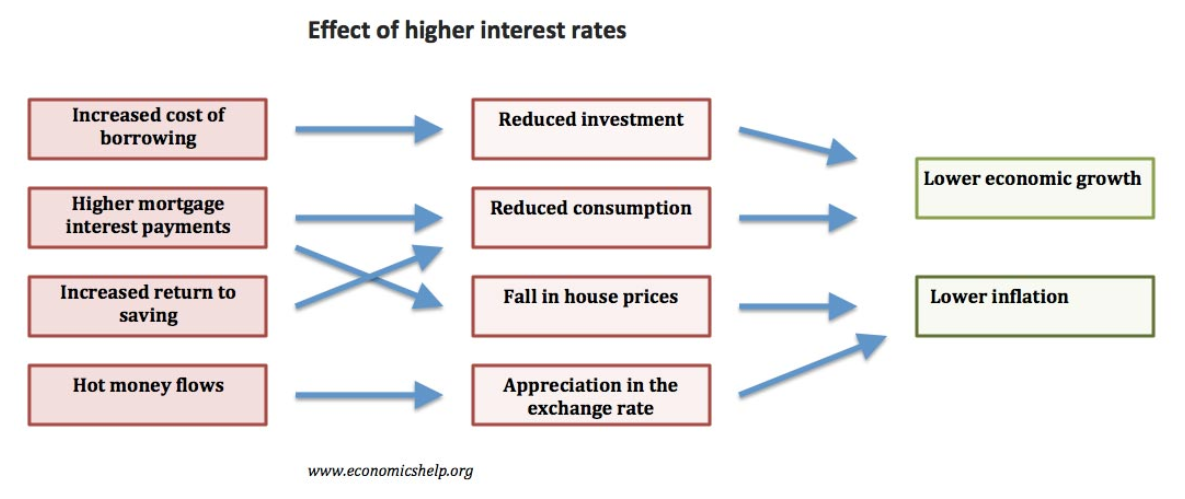
\includegraphics{images/high_rates.png}
%     \caption{}
%     \label{fig:my_label}
% \end{figure}

\chapter{HOUSING}
\begin{chapquote}{Peter Todd}
``You can never really know if something is secure. You only know when it’s been exploited and no longer secure.''
\end{chapquote}

\section{Home equity and personal balance sheets}\label{home_equity}

An asset is something that is going to give you some economic benefit. A liability is an economic obligation to someone else. The equity is the difference between assets and liabilities.
Assume I have \$250k in cash, no assets, no liabilities. Then, I borrow \$750k from the bank to buy a \$1m house. My equity is still \$250k, but if my house, for some unforeseen reason, depreciates to 800k, then my equity will decrease. In this case, a drop of 20\% of my assets corresponds to a drop of 80\% of my equity.
Instead, in a more optimistic scenario, my house appreciates to \$1.2m, hence +20\%, my equity becomes \$450k, hence +80\%, a make-believe amount of wealth. 
In the second situation, I can go back to the bank and show them that now I have \$450k in equity, but I want cash instead. They agree to give me money, but up to 75\% of the value of my house: \$900k. Subtracting what I owe the bank, I get \$150k in cash. This money come from the equity of my house basically. Now I have \$1.2m (house) + \$150k (cash) of assets and \$750k (house loan) + \$150k (equity loan) of liabilities for a total equity of \$450k, unchanged. What I can do now, though, is to go on vacation and spend all my cash. When I come back from vacation, I'll have \$300k in equity. I was able to do this because I borrowed money against the value of my house.

\section{Mortgages} \label{mortgages}
Assume I want to buy a house but I only have 25\% of the money needed to buy it, which is \$500k. I can ask the bank for a loan for the other 75\%. The bank will give me the loan, but the home title goes to the bank to secure the loan. While I pay back my loan, I live in the house, but the bank owns it as a security. This pledging of the title is a mortgage (pledge: that will die when I pay back my loan).

Let's assume there is a 5.5\% fixed annual interest rate and it is a 30-year loan. The monthly interest rate is 0.46\% and the monthly payment is roughly \$2130. Let's analyze the table in Figure \ref{fig:mortgage_xlsx}, starting from the first line. 

\begin{figure}[h!]
\centering
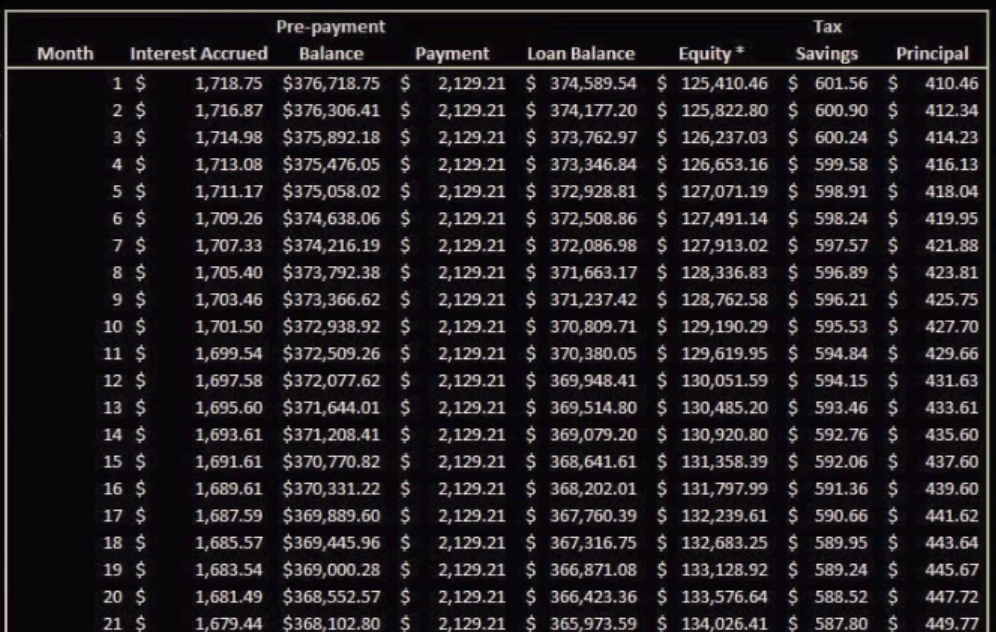
\includegraphics[width=0.8\textwidth]{images/mortgage_xlsx.png}
\caption{Mortgage spreadsheet}
\label{fig:mortgage_xlsx}
\end{figure}

The second column is obtained by multiplying \$350k by the monthly interest rate. The third column is my total debt I have with the bank which is the sum of my loan plus the interest accrued. The fourth column is simply the monthly payment. The fifth column is the total debt after the monthly payment. The sixth column is my equity, which was initially \$125k. The increment in its value is coming from the difference between my monthly payment and the monthly interest (fourth minus second column). The second line is similar, but the second column is obtained by multiplying the monthly interest rate by the fifth column of the previous row. The procedure is the same, but now I pay less interest as the loan is lower. My monthly payment is fixed, but with time there is less interest to pay and more money goes into the payment of the loan. The money paid in interest is deductible from taxes, which means I can subtract it from my income and pay less taxes. To compute the tax savings, one can simply multiply the interest accrued by the tax rate. 

\subsection{Adjustable rate mortgages}
So far, the interest rate was considered to be fixed. Sometimes, though, it is not fixed, like in the case of 5/1 ARM. This is a hybrid adjustable rate mortgage, where during the first 5 years there is a fixed rate, then it is adjustable every year―it usually lasts 15-30 years. The bank can change the rate according to some index (e.g., 10-year treasury bonds) and this is obviously riskier (interest rate risk). In the case of fixed interest rate is the lender at risk, in the case of adjustable interest rate is the borrower at risk.
\subsection{Balloon payments}
A different scenario is the "balloon payment". Here, the bank borrows money and sets a fixed interest rate for a 30-year loan, but it lasts only 10 years, which means after 10 years of fixed interest rate, the borrower has to pay back the remaining loan. This might seem a bit illogical, but it's not. In the 10 years, the borrower has less risk as the interest rate is fixed, and after that, the bank has no risk at all (this may lead the bank to offer a lower fixed interest rate). Also, the borrower might decode for this kind of payment if he plans to sell the house or take another loan if some cash is suddenly available (inheritance, for example).

\subsection{A bad situation}
Let's say you want to buy another house at \$200k, but you only have \$50k. Again you ask for a loan to the bank and you get \$150k. Unfortunately you lose your job and you can't pay the loan anymore and in addition the house has lost its original value and you're able to sell it for \$120k. That's not a good situation and you have two options: foreclosure, where you basically default and you're reported to credit agencies or short selling. In the latter case, you ask the bank to accept your house at \$120k and forgive you about the missing \$30k. In addition you should specify the bank not to be reported to the credit agencies, otherwise you won't be able to get another loan in many years to come. The missing \$30k though as to be considered as part of your income.

\subsection{Loan and present values}
How to compute the monthly payment seen in Figure \ref{fig:mortgage_xlsx}? Let's assume the amount of the loan is $L$, the monthly interest is $i$, $n$ is the number of months and $p$ is the monthly payment we're looking for. My first monthly payment will be:

\begin{equation}\label{eq:1monthly_payment}
p_1 = L(1+i) ;
\end{equation}

while the second would be 

\begin{equation}\label{eq:2monthly_payment}
p_2 = \bigg(L(1+i) - p_1\bigg)(1+i);
\end{equation}

and so on with the third, fourth, ..., till the n-th.
We want to pay always the same amount per month, which means: $p_1 = p_2 = ... = p_n = p$. What we also want is that after all the n payments, there is no more debt, so the loan has been covered. If we solve equation~\ref{eq:1monthly_payment} for $L$ and then again we solve equation~\ref{eq:2monthly_payment} for $L$ we would see a pattern which is the following:

\begin{equation}\label{eq:loan_sum}
L = p\sum_{j=1}^{n} \dfrac{1}{(1+i)^j};
\end{equation}

What is this? The loan can be seen as a sum of the present values of all my payments in the future (future value discounted by the interest rate). Equation~\ref{eq:loan_sum} is a geometric series and the solution is known. It turns out that $p \cong \$1200$ 

\section{Home buying process}

\subsection{Titles and insurances}
When someone is buying a house, she has to make sure that the supposed-to-be owner of the house is able to provide a document certifying that he's the real owner (possession is not always ownership). This document is called title or deed. Suppose a house is built and owned by Alice and when she dies she has absolutely no relatives to inherit the property and it is given to the city council and then sold legally to Bob. What if after 20 years, Carl shows up proving that he was the son of Alice and the house should belong to him? Bob would be in a very bad situation. To protect Bob from rare events like this, there are title insurances that will cover the costs.

\subsection{Escrow accounts}
Another critical situation arises when a buyer and a seller agree on a contract: the seller will give the title of the house to the buyer and the buyer will pay the house to the seller. But, should the buyer pay first than receiving the title or should the seller give the title before the payment? They can't trust each other, so what happens is that they need a trusted third party, an escrow agent and they open an escrow account. It will make sure that once all the money has been collected, the title is given to the buyer. After that, the escrow account is closed.

\chapter{INFLATION}
\begin{chapquote}{Al Greenspan}
``Bitcoin is not a rational currency. The United States can pay any debt it has because we can always print money.''
\end{chapquote}

\section{Inflation basics}

Let's say a year ago you selected 10 products (or services) that were widely used by the population of your country and the total cost was $S_0$. Today, you select the same 10 products and you discover that the total cost is $S_1 = rS_0$. If $r > 0$ we say that we had a price inflation. If the central bank is instead printing more money, that is monetary inflation. The consumer price index (CPI) is related to the first kind of inflation. It has different voices like food and beverages, housing, transportation, education and more, and each of them is weighted on the disposable income of a citizen. For housing, the percentage is very high and its wrong value led to financial crisis in the past. The Case-Shiller index fixes this problem. The government would like to keep the inflation low otherwise it would have higher costs for social security for example.

In Figure \ref{fig:good_economy} a good economy with moderate inflation is represented. If we have high employment, people can spend more and the prices will go up and companies will make more profit increasing production and supply which in turn will meet the demand.

\begin{figure}[h!]
\centering
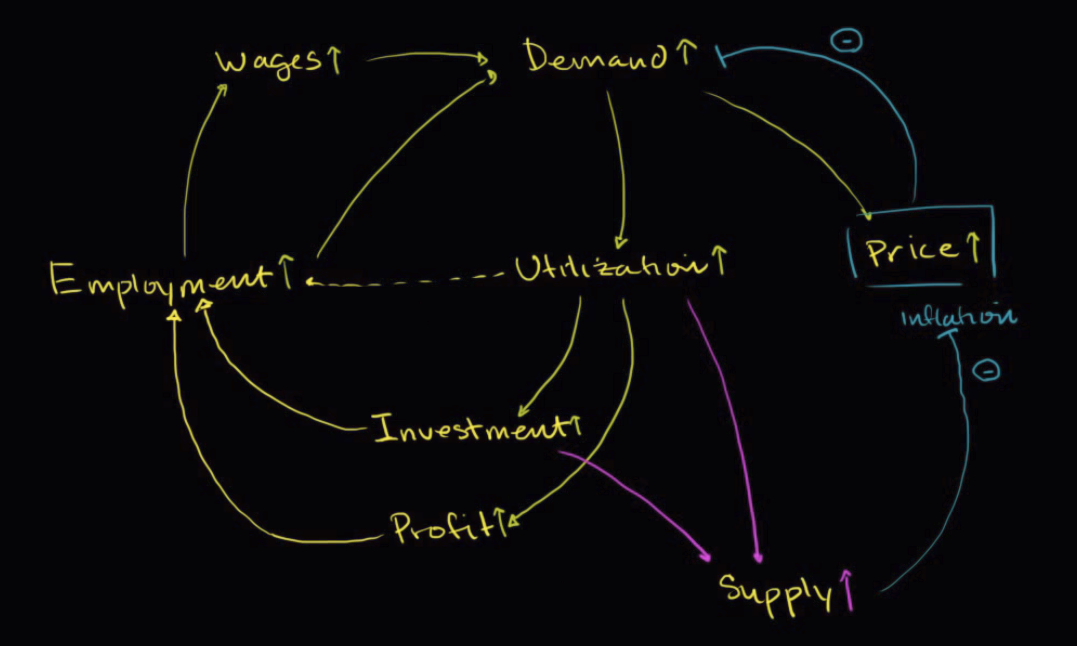
\includegraphics[width=0.8\textwidth]{images/good_economy.png}
\caption{A good economy}
\label{fig:good_economy}
\end{figure}

Another scenario is when the supply of a certain product suddenly decreases. Here, prices would go up, but there is not an increment in the demand because there is no increment on wages and not more profit. The result is stagflation, where prices are high, but people do not tend to spend more.

Hyperinflation happens when a central bank starts printing money because the government has no other way of getting money. This leads to higher prices as more money is available. This in turn leads to printing more money as the employees would start demanding more money to pay the products. If the price of a product keeps going up, then it's better to buy it and keep it (hoarding) as it will value more in the future. If no one wants to sell a product but everybody wants to buy it as it is getting value, there will be higher and higher demand increasing prices even more. Famous examples are: Weimar Germany after WWI, Zimbabwe, Hungary after WWII.

\section{Real and nominal return}

Assume one year ago I put a sum of money $S$ into the bank with an interest rate $r$, which means I have today $S' = S\cdot (1+r)$. I can think of $d = S'-S$ as my profit of this annual investment. But is it really true? In one year we may have a different inflation, suppose it has increased of $i$. This means that a product priced $S$ one year ago, is now $S_i = S \cdot i$. Hence, the return in today's money is $d_i = S' - S_i$ and the real return is:

\begin{equation}\label{eq:real_return}
r_i = \dfrac{d_i}{S_i} = \dfrac{S' - S_i}{S_i} = \dfrac{(1+r)}{(1+i)}-1.
\end{equation}

Equation \ref{eq:real_return} can also be seen as: the nominal interest rate $(1+r)$ is equal to the real interest rate $(1+r_i)$ compounded by the inflation rate $(1+i):$

\begin{equation}\label{eq:nominal_rate}
r+1 = (r_i + 1)(1+i).
\end{equation}


\section{Capacity utilization and inflation}

When starting up a business we have an initial capital $S$ and then we start thinking about the operating costs per year $C_{op}$, the costs for producing the good $C_g$, the price $p$ of the good, the number of goods you estimate to be able to produce per year $N_y$. After one year you, sold $N$ goods with a revenue $R = N \cdot p$. Considering the costs of goods $COGS = C_g \cdot N$, your gross profit $P_g = R - COGS$. Deducting the operating costs, also called overhead, you get the operating profit $P_{op} = P_g - C_{op}$. 
In an open market with competition, if a business is using a small part of its capacity, it should lower the prices so that it'll use more of its capacity. If it is instead using a big part of its capacity, it should increase the prices and maybe make more profits. In general, utilization of capacity determines inflation or deflation. Usually, capacity is correlated to demand and velocity (see below). When the average utilization is around 80-85\%, it means there is someone at 70\% and someone at 95\%. The latter ones usually start increasing prices entering a phase with increasing inflation. This can be seen in Figure~\ref{fig:inflation_utilization}. Dotted-light-blue lines represent 80-85\% of utilization. The light-blue bottom line is zero inflation. Below that line we have deflation. This means that from the '70s we've always had inflation. Interesting to notice that right before the '90s there was high utilization, but it didn't exceed 85\% and inflation didn't explode.

\begin{figure}[h!]
\centering
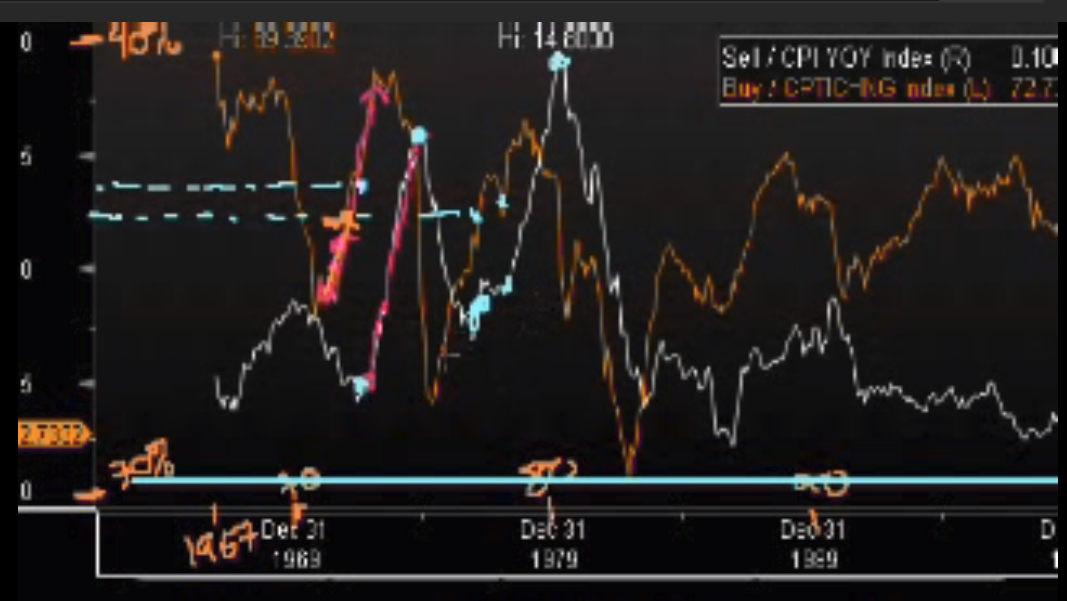
\includegraphics[width=0.8\textwidth]{images/inflation_utilization.png}
\caption{Inflation (white) and utilization (orange). Dotted-light-blue lines represent 80-85\% of utilization. The light-blue bottom line is zero inflation. High utilization is followed by high inflation twice between 1969 and 1979.}
\label{fig:inflation_utilization}
\end{figure}

On the other hand, an increase in money supply from central banks does not necessarily lead to higher demand―hence higher utilization―in that the consumer might fear to spend and thinks the market is not favourable somehow.
An equation used to describe this situation is the following:

\begin{equation}\label{eq:money_supply}
M \cdot v = p \cdot Q
\end{equation}

where $M$ is the total money supply, $v$ is the velocity of money i.e., how often it is exchanged on the market, $p$ is the average price of goods and $Q$ is the total quantity of goods and services. One can see that higher money supply lead to higher prices or higher utilization only if velocity is constant, but that's not always the case.


\begin{figure}[h!]
\centering
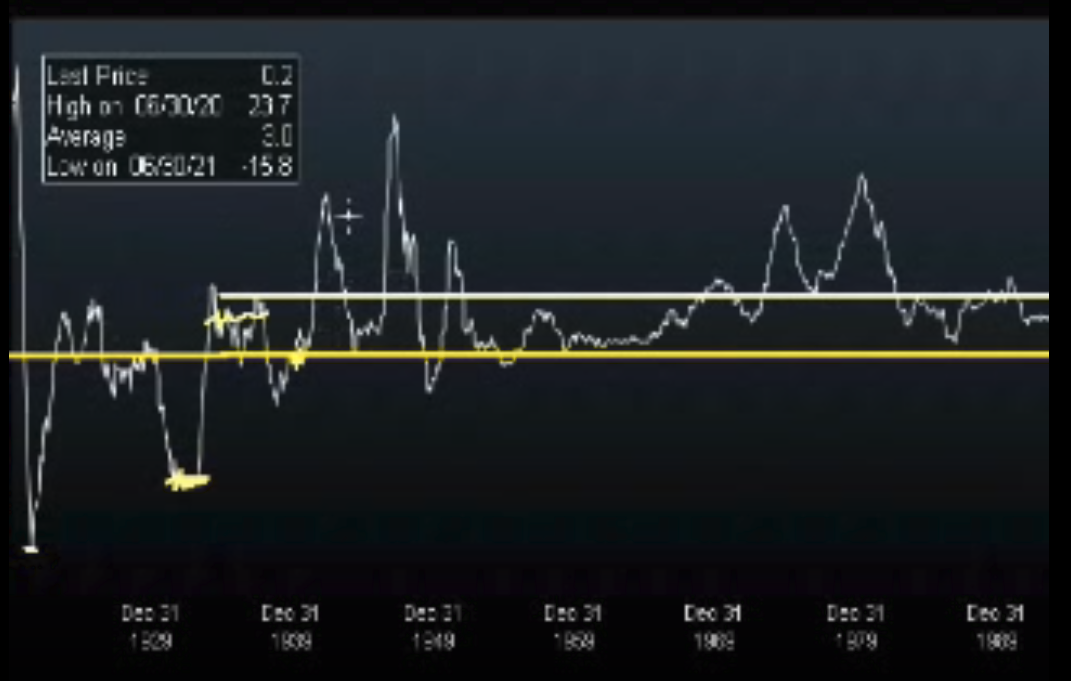
\includegraphics[width=0.8\textwidth]{images/deflation_inflation.png}
\caption{Inflation. Yellow line is zero inflation, white line is 5\% inflation, usually considered critical threshold. Few deflationary periods happened in the last century. Among them, the Great Depression in the '30s.}
\label{fig:deflation_inflation}
\end{figure}

Let's assume a country has an annual output, or Gross Domestic Product of $GDP$, a percentage of it is consumed\footnote{Consumption is spending money on stuff that will lose value, for example, when you buy a sofa the value of the sofa goes down so the money effectively disappears and you can't get it back. The opposite of consumption is investment, where you spend money on something that will (hopefully) increase in value later on, so you get more money back.}, say $c$, and the rest is for savings. These savings are usually turned into investments for the next year so that the output can increase, meaning that people get paid more and spend more and the standard of living will go up. Generally, if there are no savings, there are no money for investment and the output will decrease. In 2007, the United States consumed more than their output meaning that they "borrowed" output from other countries, such as China. A realistic scenario is that the US bought products from China using USD as a currency and, as time goes by, the amount of dollars in China increases. But US dollars are not accepted in China, hence the Chinese end up with a lot of dollars to spend. What do they buy? They buy US bonds, essentially US debt. In addition, the US was not able to save as everything was consumed and if they need money for investments, again they have to borrow more output from other countries. High consumption, by itself, attracts foreign investments. The problem appeared when people were not able to pay their (home equity) loans. Banks lost money. Liquidity was gone. People could not borrow money, nor buy. Demand and consumption went down. Utilization went down. Prices went down. Wages went down. Deflationary cycle's fear was real. By printing money, the government tries to borrow money so that people start spending, demand and consumption go up again and inflation is back. 

If the output of a country is $GDP$, a fraction of it is for taxes, another fraction is for businesses' savings and the rest is disposable income. In Figure \ref{fig:saving_rate}, the saving rate is represented from 1972 to 2008 and one can clearly see the decreasing trend. Before this period, the saving rate was around 10\%. One theory is that in the last years people had perceived savings near 10\%, but real saving was dropping because people were using credit to make more purchases than they should have been. As we approached zero, it all started collapsing because people finally realized that the credit they used to buy stuff was actually backed from savings that didn't really exist. After that, people was unable to spend and average savings went up again as depicted in the last part of the plot because people were not able to spend more than what they had (previously they were offsetting the savers).

\begin{figure}[h!]
\centering
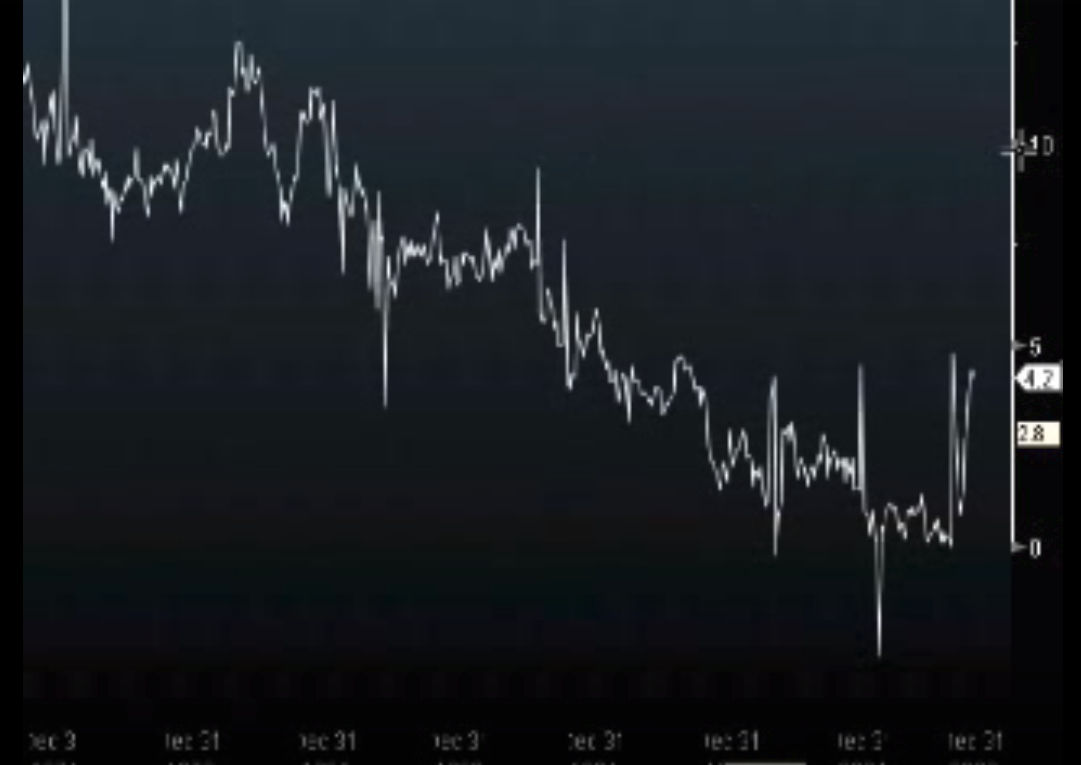
\includegraphics[width=0.8\textwidth]{images/savings.png}
\caption{Saving rate from 1972 to 2008.}
\label{fig:saving_rate}
\end{figure}

\chapter{TAXES}
\begin{chapquote}{Associates of Edwin L. Drake in 1859}
``Drill for oil? You mean drill into the ground to try and find oil? You're crazy.''
\end{chapquote}

\section{Personal taxes} \label{Personal taxes}

Figure \ref{fig:tax_rate_schedule} summarizes the US income tax rate schedule. As already said in section \ref{mortgages}, deductions are possible when paying interests, so it is possible that two people with the same income end up paying a different amount of taxes. 

\begin{figure}[h!]
\centering
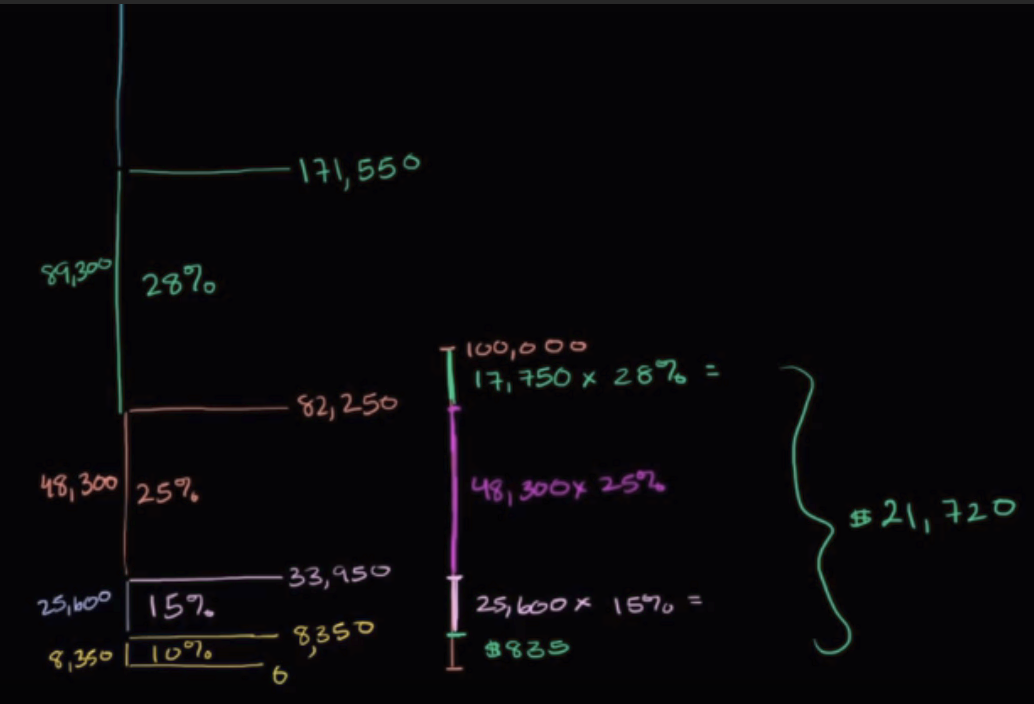
\includegraphics[width=0.8\textwidth]{images/tax_rate_schedule.png}
\caption{US income tax rate schedule.}
\label{fig:tax_rate_schedule}
\end{figure}

Sometimes it may happen that due to lots of deductions from an income, one can end up paying very low taxes and when they are less than a certain sum $AMT$, then this second sum is paid instead.  Alternative Minimum Tax (AMT) is a tax computed similarly to Figure \ref{fig:tax_rate_schedule} but with different tax rates and, as the name says, it is a minimum tax that every US citizen has to pay.

The estate tax, also known as inheritance tax, allows you to give all of your money, properties and so on, to someone when you pass away without any tax. If your estate is more than \$5 millions, say $S$, then you'll pay 35\% of taxes on the remaining part: $T = (S - \$5M) \cdot 0.35$. The reason behind this tax is that it exists only for very rich people and it's an incentive to make rich children start working or "a certain corrective against the development of a race of idle rich" as W. Churchill said in 1924. Also, this tax may look like a double-taxation system as we already pay taxes on our income, but in fact double taxation already happens everyday when we buy a product (VAT). 

In the US, there are taxes paid to the federal government and some states also add other state taxes. Different deductions are possible, depending on your status. If you're married you usually end up paying more taxes. This is known as marriage penalty, but this does not always occur. Some examples are reported in Figure \ref{fig:marriage_penalty}. 

\begin{figure}[h!]
\centering
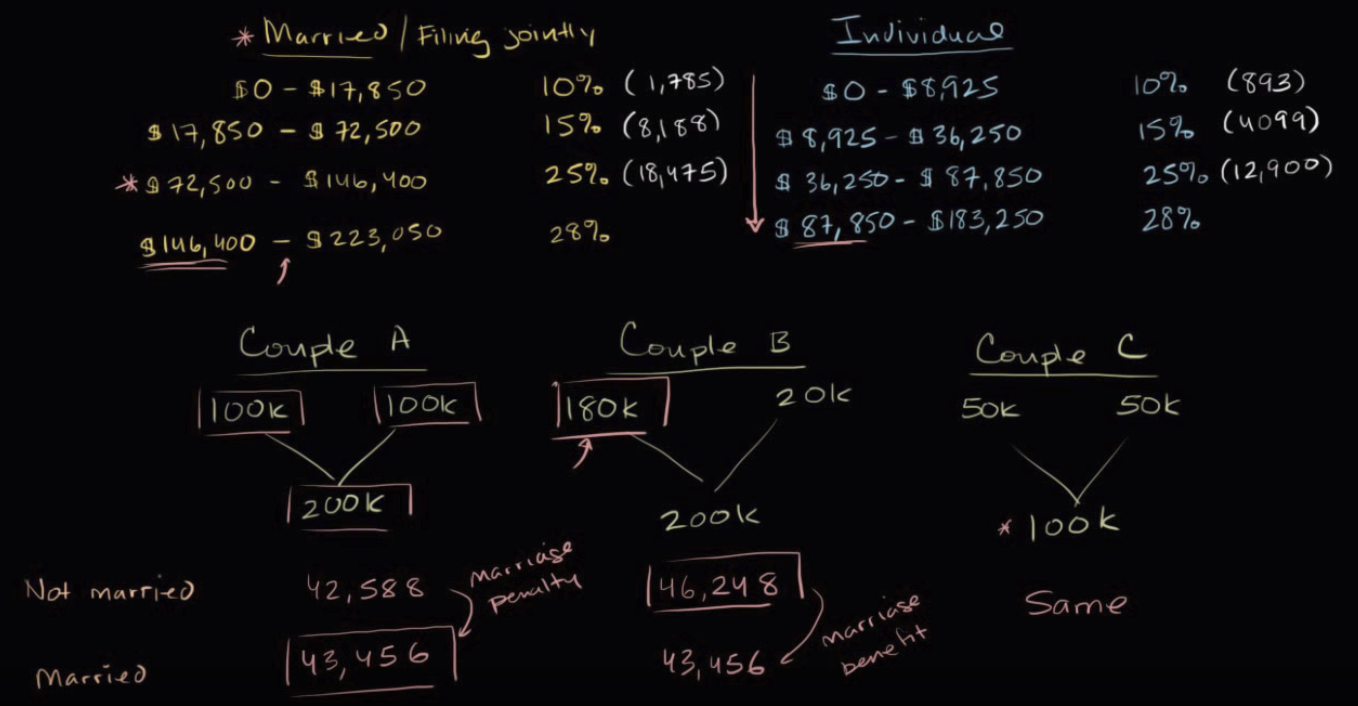
\includegraphics[width=0.8\textwidth]{images/marriage_penalty.png}
\caption{Different examples of marriage taxation.}
\label{fig:marriage_penalty}
\end{figure}

If paying taxes as married and filing jointly does not mean lower taxes as in the first example, you may think to pay separately, but that's not an option. You'd fall under the "filing separately" option where you end up paying the same amount of taxes as can be seen in Figure \ref{fig:marriage_separately} 

\begin{figure}[h!]
\centering
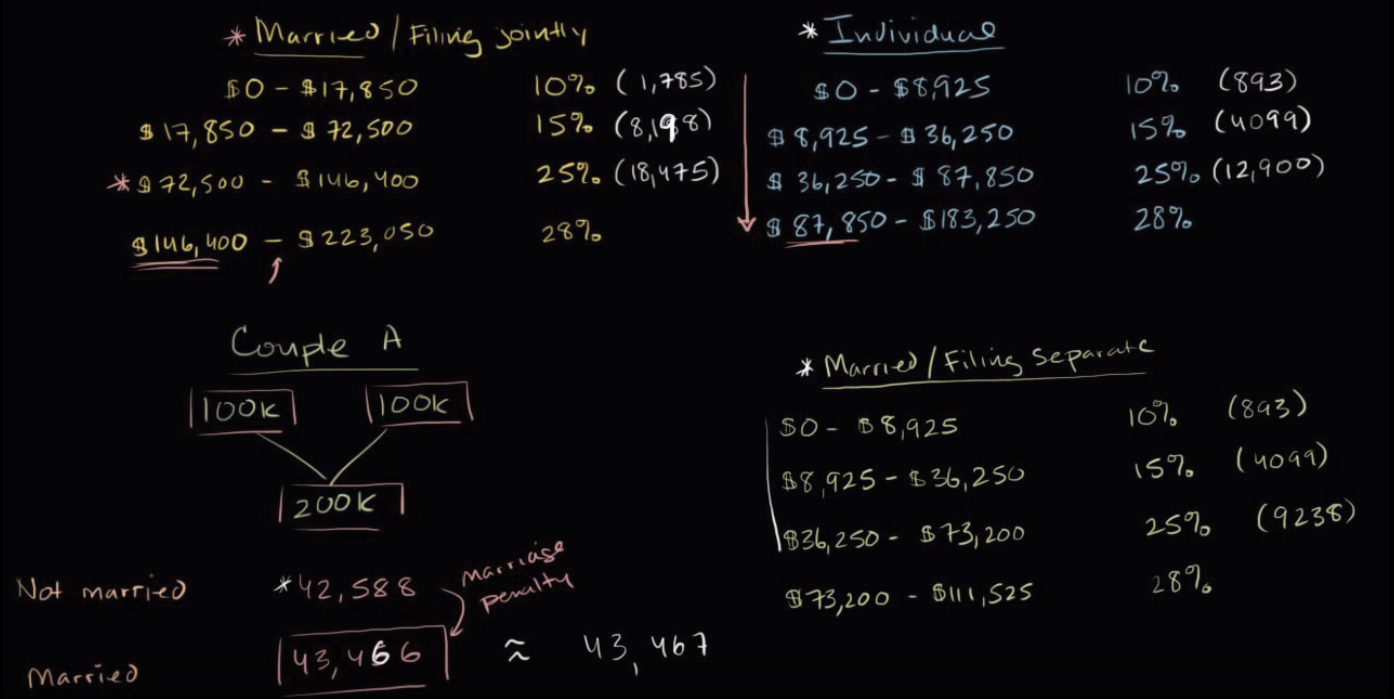
\includegraphics[width=0.8\textwidth]{images/marriage_separately.png}
\caption{Married, filing separately.}
\label{fig:marriage_separately}
\end{figure}

\section{Corporate taxation}

A corporation is a legal entity that can "act" like a person. It has limited liability and its ownership can be shared. The corporation has a certain amount of capital coming from the founders (or owners and investors), but if something bad happens, like an accident or a natural disaster, then the corporation can go bankrupt and all the money of the company is gone, but the owners do not lose their own private assets unrelated to the corporation. Being protected from this kind of events encourage entrepreneurship and starting a business, but it also levels all the possible entrepreneurs, in that a rich businessman with lots of assets and a simple middle-class person can both decide to start a corporation with an initial capital $C$, without being afraid of losing other money. The counterargument to this is that when the corporation goes bankrupt there will be someone else losing money. This is a trade-off in modern society.

There exists different types of corporations. The biggest one is a C-corp, such as big public companies. They will have a double-taxation system where the company pays taxes, but also the shareholders pay taxes on their profit. Other smaller corporations include: LLC, LP, LLP, S-corp. They have a single taxation. 

Some companies may also create a subsidiary in another countries with lower taxes and report the bigger part of their gross profit coming from the other countries ending up paying considerably less taxes. Nevertheless, if a company claims to have a large amount of money coming from abroad (where it pays less taxes) they have to send it back to the initial country (with higher taxes) somehow. In this last step, usually, there is a tax to prevent this kind of illicit transactions.

\section{Additional notes}

\subsection{Tax selling}
Imagine you have just sold stocks from company A and you made a profit of \$1k and this is all your profit for this year. If you had to pay taxes on this profit with a rate of 20\%, you'd pay \$200. Assume that you also have 100 stocks from company B that you bought for \$10 each and they are now trading at \$5, with stable or non-increasing trend. So, before the tax season, you decide to sell stocks B and lose \$500. Now your profit is \%500 and your taxes are \$100. Hence, the purpose of tax selling is to sell assets that are in a loss position for you without a positive trend in the near future and reduce your taxable income.

It is important to note that the IRS is aware that the deductibility of investment losses might tempt investors to sell at a loss, deduct the loss, and then turn around and buy the same stock again in an effort to evade taxes. This practice is called a wash sale, and the IRS has wash sale rules in place to prevent investors from selling and buying back stocks to avoid paying taxes.

\chapter{ACCOUNTING AND FINANCIAL STATEMENTS}
\begin{chapquote}{Unknown}
``Lotteries are simply “a tax on people bad at math”''
\end{chapquote}

\section{Cash versus accrual accounting}
Cash accounting is when you get cash from a customer and you count that as revenue for the current month. And any time you have to spend cash, you count that as an expense, again for the current month. This is what most small businesses do, while most slightly more sophisticated businesses would use accrual-based accounting, because that matches up the actual expenses and the revenue a little bit better in each period. 
The whole idea with accrual accounting is to match your revenues and expenses to when you actually perform the service. So it actually captures business activity, as opposed to just capturing when cash changes hands. Figure \ref{fig:cashVSaccrual} sums up the two accounting systems.

\begin{figure}[h!]
\centering
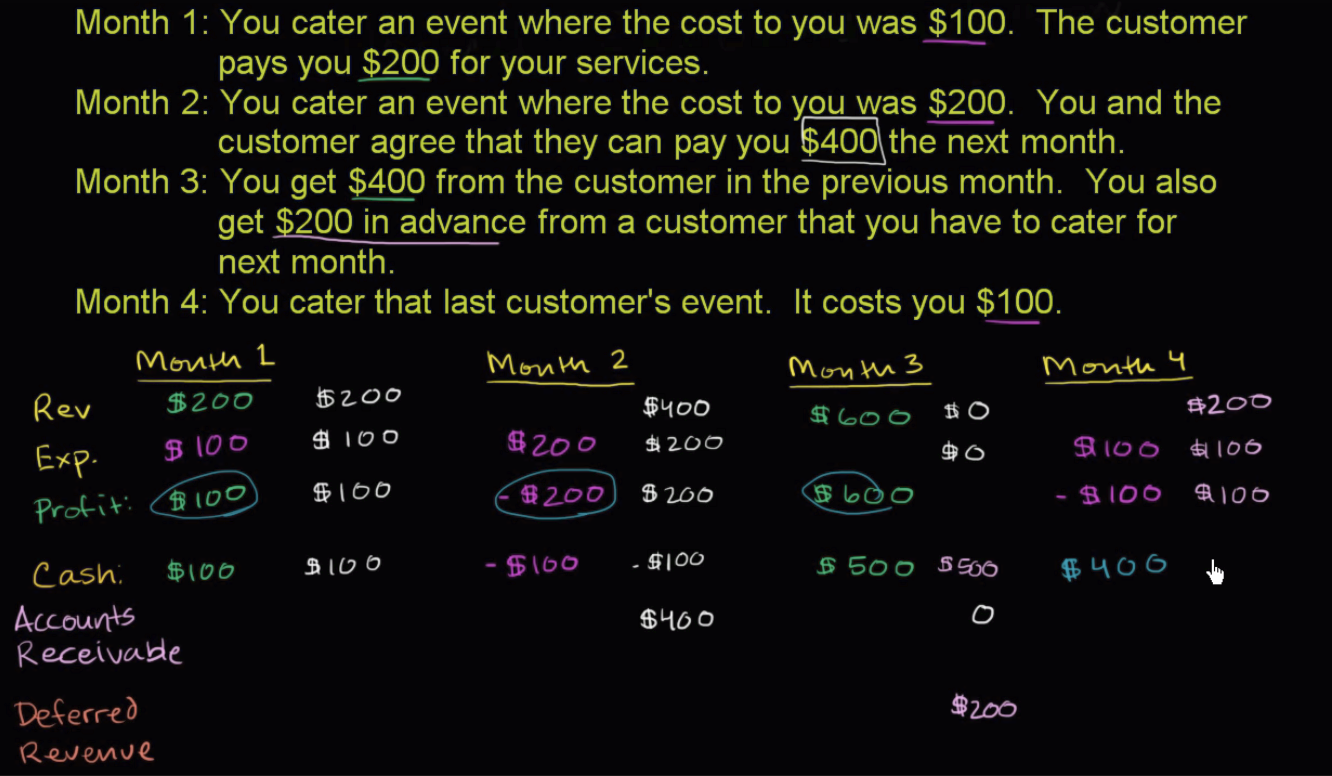
\includegraphics[width=0.8\textwidth]{images/cashVSaccrual.png}
\caption{Cash-based accounting (purple and green) vs accrual-based accounting (white). You should replace the hand pointer with \$400.}
\label{fig:cashVSaccrual}
\end{figure}

\section{Three core financial statements}

The income statement tells you what happens during a time period, while balance sheets are snapshots in time where you can see the cash (positive or negative, in which case would be debt to the bank for example), accounts receivable (money that you'll get in the future), deferred revenues (money that you have already received but you'll use in the future) and the resulting equity. The equity of a month corresponds also to the sum of the equity of the previous month plus the income reported in the income statement.

To keep track of what happens at a cash level, we have the cash flow statement. As we see from Figure \ref{fig:cashVSaccrual} in the cash line, at the end of the first month we have +\$100 and at the end of month 2 we have -\$100 nevertheless during month 2 according to the accrual-based accounting we made a profit of \$200. This is because we have the accounts receivable of +\$400. In the cash flow statement, we start from the cash at the end of a month, month 1 for example, we sum the net income, we subtract the accounts receivable (because we still don't have the cash) and we sum the deferred revenues (because we have the cash already). The result is the cash we get at the next month, month 2 in this case.

The historical cost is the amount of money spent on some initial good to start a business (land, factory, machines), while the fair value is how much they are worth now in the market, independently of the historical cost.

\section{Depreciation and amortization}

Depreciation and amortization spread the cost of an asset on its whole lifespan. The difference is that the former is for tangible assets (e.g., machines) the latter is for intangible assets (e.g., licenses, I.P.). 

\chapter{STOCKS AND BONDS}
\begin{chapquote}{Ariel Deschapell}
``While traders may move the markets, it is the tinkerers that will truly determine the future.''
\end{chapquote}

\section{Introduction to stocks} \label{Introduction to stocks}

If you own shares, also known as stocks, you are a part owner of a company. If you own bonds, you are part lender to the company. A company, just like a normal person, has assets, say $A$, and liabilities, say $L$, with a resulting equity $E = A - L$. Let's assume also that the company decides to have $N$ shares. This means that the value of each share is $V = \dfrac{E}{N}$. So, if you own $n$ shares of this company, you'd have a total amount of $S = V \cdot n$. Now, $A$ and $L$ are values provided by the company itself, but the market may perceive the value of the company in a different way. This means that people may be willing to sell and buy shares for a price different from $V$, say $V'$. If the company is known to have a good outlook, then $V' > V$. The market capitalization is simply $C = N \cdot V'$, which can obviously be different from the equity $E$.

There are two ways for a company to raise money: by borrowing money (debt) or by selling shares (equity). A security\footnote{A security is something that can be bought and sold that has some economic value. Possible categories are: debt securities (e.g., banknotes, bonds), equity securities (e.g., common stocks), derivatives (e.g., forwards, futures, options, and swaps).} in the former case is a bond, while in the latter is a stock. As we can split the equity in shares, we can split liabilities in bonds\footnote{Of course, we can have part of liabilities in form of loans with banks instead of bonds with the market.}, meaning that our debt can be owned by someone with these bond tickets. This ticket says the company will pay back the money to its owner at maturity. A stock is different in that its ownership does not mean the company owe me money.

\section{Shorting stocks}

Let's say I have reason to believe that the stocks of company X are going to lose value in the near future. The current share value is $V$. What I do is going to a broker and ask him to borrow\footnote{When borrowing stocks, in general there is a upfront payment of 50\% of the stock value.} me some stocks, say $n$ from company X. Let's assume the broker has $N$ stocks from company X owned by some of his other clients and he's able to lend me $n$ stocks\footnote{Once I have the shares, it is still as if the original clients own the stocks, so if there are dividends from the company I have to pay for them to the original owner of the stocks and the broker has to make sure that everything plays out smoothly. The original owner of the stocks is aware of her stocks being borrowed to me, but she can still sell them. To do this, the broker will give her stocks from another of his clients and then it's as if I borrowed the stocks from this second client.}, where $n < N$. Then, what I do is to sell these $n$ stocks to the market and I get a revenue of $R = n \cdot V$, but I still owe $n$ stocks of X to my broker. Luckily, after some days the value of the stock decreases by 50\% and I decide to cover and buy $n$ stocks from the market spending $C = n\dfrac{V}{2}$ and I give them back to my broker. At the end, my profit is $P = R -C$. In this case I'm the short seller: I borrow and sell high (shorting) and I buy low (covering), while long sellers are people who buy low and sell high. A regular trader would make money by buying low and selling high and buying low and selling high and so on. Depending on where you start from, you are a good long-seller or a good sort-seller.

In this case, the short seller (me) was lucky because the company's shares did lose value. What if the shares went up instead? Imagine that, as time goes by, the share's value keeps increasing. The more I wait to cover my stocks (buying them from the market and giving them back to my broker) the more the money I lose. In this short-selling scenario, there is absolutely no limit to the money I can lose. If the company keeps reporting good results for years, I may end up with a huge amount of money to pay back to my broker. In the case of long selling instead the worst case scenario is me losing the initial amount of money I used to buy stocks, which is limited, whatever the losses of the company. 

In a financial market with only good short-sellers, the volatility of the market would be reduced. Why? A successful short-seller would sell when the stock value is high, and if there are lots of successful short sellers the value of the stock would decrease, (simply because there is more stock supply). When the stock value is low instead there are a lot of buyers and the stock value would increase (simply because there is more demand). Bad short-sellers would make the stock more volatile instead, but they will disappear soon from the market as they'll lose lots of money for being bad short-sellers (buying high and selling low). In general, the owners of a stock don't like volatility.

The are two types of people in the financial market: the ones who are positive and the ones who scrutinize. The first group wants markets always to go up. They report good news, try to hide problems to avoid losses. Some examples are companies' management, banks, governments, ads sellers (mostly financial press), rating agencies (paid by banks). The second group is basically made of short-sellers, who try to find problems in companies, banks and governments. They try to make sure that the value of stocks, and in general the markets, are not overvalued. They can be seen as being in the society's side in preventing bad behaviours from the positive group. Of course, there may be some exceptions such as people spreading rumours and manipulating the markets.

\section{Understanding company statements and capital structure}

As seen in section \ref{Introduction to stocks} the market capitalization $C$ can differ from the owner's equity $E$ if the market as a different view compared to the company's books. If the market capitalization is higher than equity, it means that the company has an intangible asset, which could be the brand itself, the management's expertise or the location for example. What if the market cap is lower than equity? It means that the assets of the company do not actually worth that much.

\section{Corporate metrics and valuation} \label{Corporate metrics and valuation}

By selling a product, a company gets revenues, from which it subtracts the cost of the products, resulting in the gross profit. Then it subtracts other additional costs generally known as Selling, General and Administrative Expenses (S\&GA)\footnote{Direct labor is employees who are directly involved in making the product, who "touch the product." The labor cost is included in cost of goods sold. Everyone else is considered indirect labor and included in SG\&A.} to obtain the operating profit $P_{op}$. The return on asset is then computed as $ROA = P_{op}/A$, where $A$ is clearly the assets of the company. If the company owns some stocks or other financial assets, then the real return on asset is $ROA = \dfrac{EBIT}{A}$, where the numerator stands for earnings before interests and taxes which is equal to the operating profit (profit coming from the operating assets) plus the profit from financial assets that the company owns. This second definition is a bit more informative than the previous one. In general the return on asset tells us how good a company is in turning its assets into money, ignoring loans and taxes.

Some companies though may have some liabilities, such as loans to banks, so they need to subtract the interest to pay from the operating profit obtaining the pre-tax profit\footnote{Most companies pay the interest on the debt rather than paying the principal of the debt because they will have higher deductible taxes.}. As expected, from the pre-tax profit one must subtract taxes to get the net income $I_{net}$, also known as earnings, usually reported a TTM (trailing twelve months). Another index for evaluating a company is the return on equity $ROE = \dfrac{I_{net}}{E}$. This indicator could also be seen as how good the company is at dealing with loans and taxes.

If a company has $N$ shares, then the earning per share is $EPS = \dfrac{I_{net}}{N}$. Instead, the price to earning ratio is $P/E = \dfrac{V'}{EPS} = \dfrac{NV'}{I_{net}}$, where $V'$ is the value of a share determined by the market, which can, as already said, differ from the book value per share $V$, determined by the accountants of the company. What's the meaning of this $P/E$\footnote{Be careful: the denominator stands for earnings and not equity.}? It represents how much money you have to invest on a single stock to get a profit of one dollar (or any other currency). Obviously, the lower the better because a small numerator and a big denominator means I pay few for something that will give me more. If you look at it from another perspective, namely its inverse, $E/P$, it can be seen as the percentage of profit you make with an investment. If an earning per share $EPS$ is always constant and the price to earning ratio $P/E$ is low (or equivalently a high $E/P$), you should invest on that company rather than putting your money into the banks which usually offer a lower interest rate compared to the $E/P$ of the company―because banks bring less risk in general\footnote{Usually banks offer few percent points in interest rates, say 2\% which means a $P/E$ of 50.}. Usually, companies are analyzed in depth to assess their future earnings or equivalently their future $EPS$, and the final result of all the analysts is averaged and a consensus is expressed in the so-called forward earnings. These are sell-side analysts from investment banks and research houses that are trying to sell financial products. In contrast we have buy-side analysts, namely people from hedge funds that must decide where to invest.

If two companies have two different $P/E$ ratios, it is not always better to buy the one with the lower value. Why? First of all, the one with lower value may be more risky. Second, the one with higher value might be growing and its $P/E$ will decrease. You can also see it in this way: if a lot of people are willing to pay a high price for a stock, it means the company is believed to grow, if instead the price is low, maybe the stock is not very interesting for the market. A low PER can indicate either that a company may currently be undervalued (people do not believe in the company despite its profit) or that the company is doing exceptionally well relative to its past trends.

An individual company’s P/E ratio is much more meaningful when taken alongside P/E ratios of other companies within the same sector. For example, an energy company may have a high P/E ratio, but this may reflect a trend within the sector rather than one merely within the individual company. An individual company’s high P/E ratio, for example, would be less cause for concern when the entire sector has high P/E ratios.

The price to earning ratio is useful to represent the growth of a company, but it does not consider how the company is capitalized, namely how the assets are payed. The enterprise value is obtained by adding the market cap to the debt and subtracting the non operating assets (cash, financial investments): 
\begin{equation}\label{ev}
    EV = C + L - A_{non-op}.
\end{equation}
To obtain a more correct share value, an investor chooses a price to earning ratio for the company that he's willing to pay and sets it equal to the ratio between the enterprise value and the operating profit:

\begin{equation}\label{eq:pe_ev}
P/E = \dfrac{EV}{P_{op}}.
\end{equation}

From equation \ref{eq:pe_ev}, we can obtain $EV$, which then can be used in equation \ref{ev} to compute the market cap $C$. The price per share the investor is then willing to pay would be $PPS = \dfrac{C}{N}$, where $N$ is the number of shares. In this way, if two companies have the same operating profit but different liabilities and non-operating assets you'd buy stocks from those 2 companies at different prices.

Another index to analyze a company is the ratio between enterprise value and EBITDA (earnings before interests, taxation, depreciation and amortization). The difference with ROA―where the denominator was operating profit―is that here we don't consider depreciation and amortization which are non-cash expenses, rather we consider raw cash that the company is producing. EBITDA represents how much income the employees are generating by their current activities. It ignores things that employees have nothing to do with.

\section{Life of a company} \label{Life of a company}

It all starts with an idea and some unique skills. These are the only (intangible) assets of the company. The founders can issue shares to themselves and decide what is the value of their idea before starting the business. Let's assume they agree on a sum $S$, which is the pre-money valuation. What they need to do then is to find an investor. Banks are not helpful in this case, but venture capitalists or angel investors might be interested in the idea and put a sum $S'$ to start the business. This sum may be higher than the pre-money valuation and if this is the case, the investor will own the majority of the shares. Now the assets are both intangible (the idea and the skills) and tangible (the investor's money) for a total of $S + S'$, the post-money valuation. This means that the owners must issue shares for a total amount of $S'$ to the investor. 

Once the business has started―an office, employees, and so on―the founders might need additional money to go on because they didn't make much profit yet. In this case, the founders ask for help to seed venture capitalists, more professional people. The money from this seed VC investor represents the series A founding. The seed VC has MBAs and analysts for a pre-money valuation, say $S''$ which can be more, but also less than our previous assets $S + S'$, which means our shares will be worth more or less. The founders and the other owners may decide to get the series A funds also at a lower value so as not to lose the majority in the company. The post-money valuation of the company will be then $A =S + S' + S''$, assuming $S''$ is the definitive series A funding, and the owners will issue more shares to the seed VC according the new funding value. If more money is needed, the owners will raise a series B funding with other VCs and issue more shares. Up-round is when the pre-money valuation of this round is higher than the post-money valuation of the previous round. 

The problem so far is that the investors own shares of the company, but they cannot turn them into cash. The board can then decide to go public and raise a lot of money with an initial public offering (IPO). The legal work will be carried out by the legal underwriter and a syndicate (group of investment banks) will come up with a price. This price should allow the stock value to increase in the first days, so it shouldn't be too high. If the stocks are bought during an IPO, this money will finance the company, but if the stocks are traded afterwards in a stock exchange, no additional money will be received by the public company. Usually a 7\% of the money raised is payed to the syndicate. After some time, if the company needs more money, it can issue more stocks and sell them to the public market (probably a lower price as the offer increases). This is called follow-on offering.

When a company is going bad, it has two options: liquidation (called chapter 7) and restructuring. Liquidation means that the assets are sold to pay back the debt in the liabilities and then the company shuts down. The debt is layered: senior secure, senior unsecure, subordinated, junior (equity). The first level is the one which is paid first. The other option is when the shareholders think the company can still operate but the debt is too high. What happens is that the company starts chapter 11 bankruptcy and gets a new loan: Debtor In Possession Financing, which is even more senior than the senior secure, to keep operating. Then, the bankruptcy court (group of banks) will value the company (its assets) and how much debt it can have, someone will provide higher numbers (people related to the shareholders) and someone else will provide lower numbers (banks hired from the seniors). The lower the valuation, the higher the number of the shares the seniors will get, vice versa the higher the valuation, the higher the numbers of shares the original shareholders keep. The original shareholders may also give all the shares to the seniors and lose the company's ownership. People behind the DIP financing will get their share of equity. 

\section{Dilution}
When a company decides to issue some more shares to an investor, each shareholder will own a smaller fraction of the company, but the price per share is not diluted.

\section{Mergers and acquisitions}
There are two companies, company A with $N_A$ shares at a price of $p_A$ and a company B with $N_B$ shares at a price of $p_B$. Let's say that the market cap of A is higher than B's market cap, $N_A \cdot p_A > N_B \cdot p_B$. Assume now that company A wants to acquire company B. It can issue $N$ shares for a certain sum $S = N\cdot p_A$ greater than B's market cap, which means
\begin{equation}\label{eq:raised}
    S = N\cdot p_A > N_B \cdot p_B.
\end{equation}
Company B will accept these $N$ shares, because they are worth more than its market cap, but all the stocks of company B become part of the assets of company A. If this happens, it means that one share of B can then be exchanged for $N/N_B$ shares of A. If you are sure that this acquisition is going to happen~\footnote{It's not easy to know: maybe there is a monopoly risk, or another bidder.}, then you'd buy (long) a stock of B and sell (short) $N/N_B$ shares of A, before the acquisition. By shorting, you get $R = \dfrac{N}{N_B}p_A$ and by longing\footnote{I hope this term is valid.} you pay $p_B$. The nice thing here is that because of equation \ref{eq:raised}, we know that $\dfrac{N}{N_B}p_A > p_B$, so our immediate profit would be $P = R - p_B > 0$. Then, once the acquisition has happened, you can cover your short with your long position, at no costs\footnote{Cool stuff!}.

\section{Leveraged buy-outs}
Let's say there is a very stable company with an old owner willing to sell the company to you. He owns all the assets $A$, no liabilities. You are willing to buy the company but you only have money for a fraction $f$ of all the assets. The idea is to ask for a loan of $(1-f)A$ to a bank with an interest rate $r$ and since the company is very stable, it should not be too difficult. This is a leveraged buyout, meaning that with a small capital, you were able to buy the entire company thanks to a loan. Now the net income will be lower because of the interest on the debt, but the ROE will be much higher than before.

\section{Bonds}
A loan of a company is different from a loan for buying a house. In the latter case, at every payment there is a decreasing part for paying off the interest and an increasing part for paying off the debt. In the former case instead, the company is always paying the interest and at the last payment it will pay off all the principal. If cash is not available, another loan will be taken.

One way to raise money, other than issuing shares, is to take a loan from a bank, but what if instead of one single bank we ask to many more banks or any other entity in the market? The idea is to sell debt to whoever is interested using bonds. This means the company sells coupons with a principal $P$ and an interest rate $r$ with details about the maturity time (1, 2, 10 years) and the payment period (semi-annually, annually). Assume a bond with a maturity time of $T$ months and a payment period of $t$ months, then every $t$ months the company will pay $r\cdot P/(T/t)$ to the owner of the bond. At the last payment, the company will have to pay the entire principal.

When the US government or a company needs money, it can issue bonds with a certain maturity time. If it is a Treasury bond and it is between 1 month and 1 year, the bond is called t-bill, if it is between 1 and 10 years it is a t-note, if it is between 10 and 30 years it is a t-bond. The yield curve represents the annual interest rate for different maturity times. Of course, if there is a high demand of bonds, the interest rate will be high.

If yesterday I bought a bond with an annual interest rate $r$ for an amount of money $S$ and today the interest rate went up, it means that someone can buy another bond expecting to get more money than me. This means that if I want to sell my bond to someone, I have to sell it for a lower price than $S$. In case the interest rate went down, I could sell it at a sum higher than $S$.

\section{Additional notes}

\subsection{Inverted yield curve and recession}
In a good economy, the yield curve loosely resembles the square root function: Long-term interest rates are lower than short-term interest rates. Historically, an inverted yield curve was a sign of upcoming recession.

During normal growth, the yield on a 30-year bond will be three points higher than a three-month bill. However, if investors believe that the economy will be slowing over the next couple of years, and then speeding up again in 10-20 years, they would prefer to tie up their money until then, rather than have to reinvest it sooner at much lower rates.

The Treasury yield curve inverted before the recessions of 2000, 1991, and 1981. The yield curve also predicted the 2008 financial crisis two years earlier. The first inversion occurred on December 22, 2005. The Fed, worried about an asset bubble in the housing market, had been raising the fed funds rate since June 2004\footnote{I guess they did this to slow down lending money and put money into the bubble.}. By December, it was 4.25 percent. That pushed the yield on the two-year Treasury bill to 4.40 percent. But the yield on the seven-year Treasury note didn't rise as fast, hitting only 4.39 percent. That meant investors were willing to accept a lower return for lending their money for seven years than for two years. That was the first inversion. By December 30, the discrepancy was worse. The two-year Treasury bill returned 4.41 percent, but the seven-year note yield fell to 4.36 percent. The 10-year Treasury note yield dropped to 4.39 percent, below the yield for the two-year bill. A month later (January 31, 2006), the Fed had raised the fed funds rate. The two-year bill yield rose to 4.54 percent. But that was more than the seven-year yield of 4.49 percent. Nevertheless, the Fed kept raising rates, hitting 5.25 percent in June 2006. On July 17, 2006, the inversion worsened again when the 10-year note yielded 5.07 percent, less than the three-month bill at 5.11 percent. This showed that investors thought the Fed was headed in the wrong direction\footnote{Are the markets always right? }. Unfortunately, the Fed ignored the warning. They thought that as long as long-term yields were low it would provide enough liquidity in the economy to prevent a recession. They were wrong. The yield curve stayed inverted until June 2007. Throughout the summer, it flip-flopped back and forth, between an inverted and flat yield curve. By September 2007, the Fed finally became concerned. It lowered the fed funds rate to 4.75 percent. It was a 1/2 point, which was a significant drop. The Fed meant to send an aggressive signal to the markets. The Fed continued to lower the rate ten times until it reached zero by the end of 2008. The yield curve was no longer inverted, but it was too late. The economy had entered the worst recession since the Great Depression \citep{yield_inversion_balance}.
% How can this happen? One possible reason is that the central bank is announcing it will lower interest rates in the future to stimulate the economy (lower borrowing costs, cheaper money). Listening to this news, an investor could decide to buy long-term bonds now because they won't be able to get the same yield in few days if the rates actually decrease. This will create more demand for long-term bonds and more demand means higher prices, higher prices and same interest rate (assuming interest rates have not changed yet) means lower yield. Voilà. Investors will be less willing\footnote{I'm not sure why.} to buy short-term bonds with low interest rates. Less demand for short term interest rates, lower prices, higher yield, more inverted curve.

\begin{figure}
    \centering
    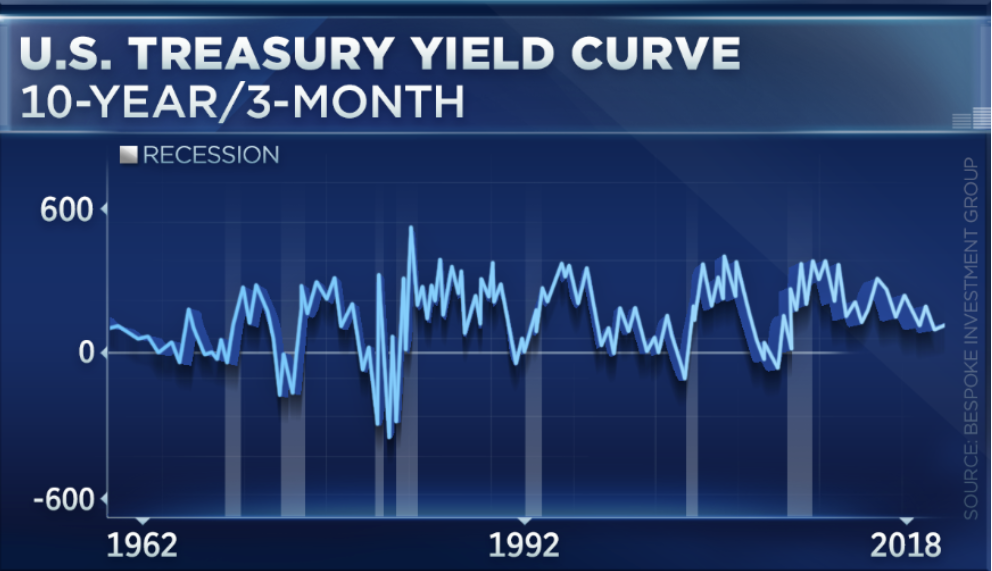
\includegraphics{images/spread_history.png}
    \caption{Spread between 10-year and 3-month bonds. Y-axis is basis points.}
    \label{fig:spread_history}
\end{figure}


\chapter{INVESTMENT VEHICLES, INSURANCE, AND RETIREMENT}
\begin{chapquote}{George Bernard Shaw}
``The reasonable man adapts himself to the world; the unreasonable one persists in trying to adapt the world to himself. Therefore, all progress depends on the unreasonable man.''
\end{chapquote}

\section{Mutual funds and ETFs}
Imagine there is a good investor with a lot of experience in finance that want to start a company. He goes to the SEC (Securities and Exchange Commission) to register his corporation (management company) and himself. Then he set up his business with come cash as asset and issues some stocks to himself. In an open-end mutual fund, anyone can ask him for stocks and become owner of the company, but the founder will keep an additional percentage of the assets for managing the business. In addition, anyone can decide to leave and cash out the stocks, so the manager must always have some liquid asset. AUM stands for assets under management. NAV stands for net asset value. The value of a share changes only thanks to good or bad investments of the manager. When shares are issued or redeemed (which happens at the end of the day), there is no change in stocks value. 

In a closed-end fund, the manager starts the business with some shares and some initial investors. After that, there is no change in number of stocks: no issuing, nor redemption. This means the manager does not need to keep cash and can invest all the assets. If a shareholder wants to cash out, she has to find an investor and sell the share in a secondary market (NASDAQ, NYSE).

To get the best of both worlds, there are ETFs (exchange traded funds). They are flexible as an open-end mutual fund, but usually only big institutions buy from or sell to the fund manager (lots of shares) and in addition these big investors can sell shares in exchange markets to the public. Usually big ETFs are not actively managed by an expert investor, rather they buy some commodities or some asset class (S\&P500, gold) so there are lower management fees.

\section{Hedge funds}
Hedge funds differ from mutual funds in that they are not regulated by the SEC therefore they can't market themselves (no ads) and can't take money from the public, only from accredited investors (a certain net income or a certain education). A hedge fund is more actively managed and has higher fees, but also the manager takes a certain percentage of the profit (around 20\% for taking the risk) called performance fee or carried interest.
In a hedge fund, the manager can have shares (called limited partner interests) of the fund, but not under his name, rather he uses a LLC. When there is a profit, roughly 2\% is the management fee, and after deducting this amount, the fund manager takes another 20\% roughly. An investor can redeem or invest money in the fund at certain points in time, so it is an open-end fund from this point of view.
The limited partners (shareholders) make sure that the general partner (fund manager) is a reliable investor. The activity of the general manager is usually not fully disclosed to the partners as it may help other traders. This secrecy is sometimes hiding some shady activity. In general, though, a hedge fund becomes dangerous for society when it is too big to fail. If it keeps a smaller size, the only people in danger are the partners. 

Venture capital and private equities are similar to hedge funds in that they have a management fee and a profit percentage, but they invest on small businesses where there is not much liquidity upfront. Hedge funds can turn assets into cash faster and easier.

Let's say I predict that the market will go up, but I'm confident one company, B, will grow more than the other, A. Then, I short a sum $S$ on company A and I long the same amount on company B. If both companies grow, but B grows more than A, I make profit, otherwise I lose money if A grows more and my prediction was wrong. If instead I predict the markets will go down but again company A will do worse than B, I make profit. Long/short hedge funds are doing this: they pick two companies and predict which one will do better (or less worse) compared to the other, regardless of the market going up or down.

When there is an acquisition incoming, where company B acquires company A paying $v'$ for each share of A, more than the current value $v$, A's shares will be traded around $V + pV$, where $p$ is a sort of market measure of the probability the acquisition will happen. If you think the acquisition will happen, you'll buy A's shares, otherwise you short, because they'll lose money. This is a merger arbitrage, a strategy of hedge funds~\footnote{"Hedge funds always find out first". GoBlue on Khan Academy's lesson}.

\section{Retirement accounts: IRAs and 401ks}
An individual retirement account is a deposit where a person puts a sum $S$ of money every year until a certain age. This money is tax deductible and can be cashed out paying a penalty and taxes on it (no penalty if after a certain age and probably there will be a lower tax bracket). This sum can be used for investments and make profit without capital gain taxes. Withdrawal is mandatory after a certain age.

With a Roth IRA (named after William Roth), you pay taxes when you deposit money %every time?%
and you won't be taxed when you cash out, even if you made big profit with your IRA. If you want to withdraw your money before a certain age, you don't pay any penalty or taxes on principal (10\% if more than the principal). A traditional IRA can be transferred to a Roth IRA. Withdrawal is not mandatory.

A 401(k) is similar to a traditional IRA but has some differences: higher % annual?
limit of money you can put in, organized by your employer, meaning that you don't manage the investments), the employer might match it (add some money), you can borrow from your 401(k) with some interest.

\section{Life insurance}
There are two possible ways to ensure life: paying a certain amount of money every year for the rest of my life or set a term so that I'll be covered for a specific period and then I won't pay anymore. Let's assume I pay $c$ per year over the next $N$ years for a life insurance of $I$. At the end of the term I would have paid $c\cdot N$, which means the company gets $c\cdot N$ on every insurance of $I$. To break even, the company must give the same insurance to $\dfrac{I}{N \cdot c}$ people and hope that at most one person dies among them during the term.

\section{Investment and consumption}
In ancient times, the word capital was used to describe any object used to produce a good such as tools, equipment and buildings. Human capital instead includes everything that make people more productive such as education, experience, talent. Financial capital is money used for the purpose of producing more output.

One possible definition of return on capital is the ratio between the amount of money made in one year and the money you invest in the business $ROC = \dfrac{S'_y}{S}$. To understand whether you should start a business you also have to take into account the costs of starting the business (interest rate of a loan). Different businesses may have different interest rates, be it for government incentives or taxation.

We can say that an investment is when money is spent to improve society. An example can be creating a factory producing cheaper cars or a family buying a house allowing their members to have a decent life. The tricky part is: what if I add a bathroom in my house? Investment or consumption? If that bathroom allows the tenants of the house to get ready in the morning faster to go to work for example, then it should be considered an investment. But if that bathroom is used only by guests and seldom, then it is considered consumption. In addition, if you consider this latter case as an investment, meaning that you think you'll find another person willing to buy the house at a higher price because of the bathroom, you are instead speculating. In other words, consumption is enjoyment, but also the loss of the opportunity to use that same money to have more enjoyment in the future. To be more precise, one can spend money for an investment and for consumption at the same time. An example is buying a purse when you really need it to be more organized at work. You can buy a simple one where 100\% of your money is invested or you buy an expensive one where, say, 20\% is investment and the rest is consumption or transfer of wealth. The money spent on advertising that purse is consumption instead, there is no improvement in society. Any activity that may waste people's time is considered consumption.

Let's imagine you have a house which you bought for $S$ and it's now yours (no debt). After 10 years, the value of your house increased and it's worth now $S'$. You feel richer, obviously, and you decide to take a home equity loan of $S'/2$ with a certain interest rate $r$ and you consume that sum say on vacation. After one year, your house suddenly loses its value and it's worth now $S''< S$. You, owner of the house, decide to give it to the bank instead of paying the loan $S'/2$ (plus interest). The bank auctions the house and gets $S''$ as planned. So the bank lost money, in particular they lost $S'/2 - S''$. If you didn't take that home equity loan, you could have sold your house now at $S''$. Instead, you lost that money. Now you're left with no house (no equity) but you consumed $S'/2$. The total amount of money lost is then $S'/2-S''+S'' = S'/2$, which is exactly the money consumed on your vacation. That sum could have been used by the bank for financing a company.

\chapter{OPTIONS, SWAPS, FUTURES, MBSs, CDOs, AND OTHER DERIVATIVES}
\begin{chapquote}{Paul Krugman}
``By 2005 or so, it will become clear that the Internet’s impact on the economy has been no greater than the fax machine’s.''
\end{chapquote}

\section{Put and call options}
Let's say you are convinced that a company is going to perform very well in the next month and its shares will increase in value. You can either buy the stock at its current price $S$ or pay a small price $f$ to have the option to buy the same stock in the future for a strike price $S_1$ and sell it within an expiry date. In this second case, you can buy the stock when you want within the expiry date. Depending on the value $S_1$ and on the value of the stock in the future, buying the option may be better than buying the stock. In particular, if the stock has a negative trend, you may want not to buy the stock and avoid losses―other than the initial cost $f$. This is the American call option, where you can buy and sell whenever you want. In the European option instead, one can sell only at the expiry date. Comparing buying a call option with buying a stock, one notices that the call option is a leverage: From a small amount of money $f$, one can have a return on investment much higher. On the other side, the worst case is the same for both: Losing 100\% of your money, either $f$ or $S$ (even if losing $S$ means the shares become worthless and its much less likely than not buying the option).
There are two payoff diagrams that can be analyzed: the value diagram and the profit-loss diagram. In both diagrams the x-axis is the stock price at expiry date. In the first one, the y-axis is how much the option is worth:
\begin{equation}\label{eq:value_diagram_call}
            f(x) = 
    \begin{cases}
        0,                  & \text{if } x\leq S\\
        x - S,              & \text{otherwise.}
    \end{cases}
\end{equation}
We can see from equation \ref{eq:value_diagram_call} that the value is always non-negative and it's linear after $x > S$.
The second diagram embeds the notion of $f$, the initial payment for the option, but the trend is similar:
\begin{equation}\label{eq:PL_diagram_call}
            f(x) = 
    \begin{cases}
        -f,                     & \text{if } x\leq S\\
        x - S - f,              & \text{otherwise.}
    \end{cases}
\end{equation}

A put option instead gives you the right to sell the stock at a specified price $S_1$ before an expiry date. In case the stock loses its value and goes below $S_1$, say at $S_2$, you can buy the stock at $S_2$ and sell it at $S_1$ and make profit. In other words, the lower the stock value, the higher the revenue. If it does not go below $S_1$ you simply don't buy the stock and you just lose $f$. A put option is less risky than shorting because in case the price goes up, you don't risk anything. As always, less risk means less reward. Put options have an American and a European version and with a price $f$, like in a call option. Also for the put option we have more leverage compared to shorting\footnote{Remember, shorting requires a 50\% upfront payment when borrowing stocks}, but the worst case is much better (100\% loss at most). The payout functions are reported in equations \ref{eq:value_diagram_put} and \ref{eq:PL_diagram_put}. 
\begin{equation}\label{eq:value_diagram_put}
            f(x) = 
    \begin{cases}
        0,                  & \text{if } x\geq S\\
        S - x,              & \text{otherwise.}
    \end{cases}
\end{equation}
\begin{equation}\label{eq:PL_diagram_put}
            f(x) = 
    \begin{cases}
        -f,                     & \text{if } x\geq S\\
        S - x - f,              & \text{otherwise.}
    \end{cases}
\end{equation}

These previous four equations are represented in Figure~\ref{fig:diagrams1}.
\begin{figure}[h!]
\centering
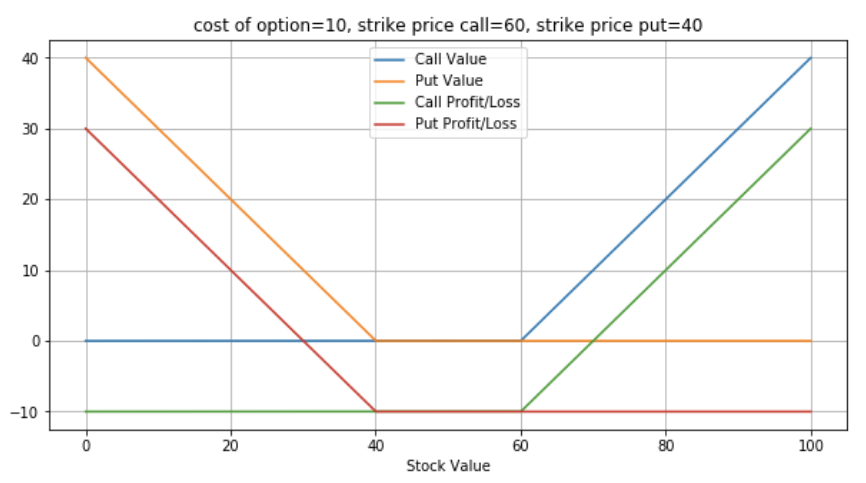
\includegraphics[width=0.8\textwidth]{images/diagrams1.png}
\caption{Value and Profit/Loss diagrams for call and put options.}
\label{fig:diagrams1}
\end{figure}

It is interesting to see what happens when one combines a stock with an option of that stock. Owning a stock can be represented simply by $f(x) = x$ in the value diagram, but by adding a put option of that stock, we get the result represented in Figure~\ref{fig:SPValue}. In Figure~\ref{fig:SPPL} the Profit/Loss diagram shows that buying a put option and the stock is like having an insurance on that stock. Ideally, you'd like to have the linear part of the green line in Figure~\ref{fig:SPPL} as close as possible to the blue line, which means a low-priced put option. The difference between the initial price of the stock and the strike price of the put option plays an important role as well.

\begin{figure}[h!]
\centering
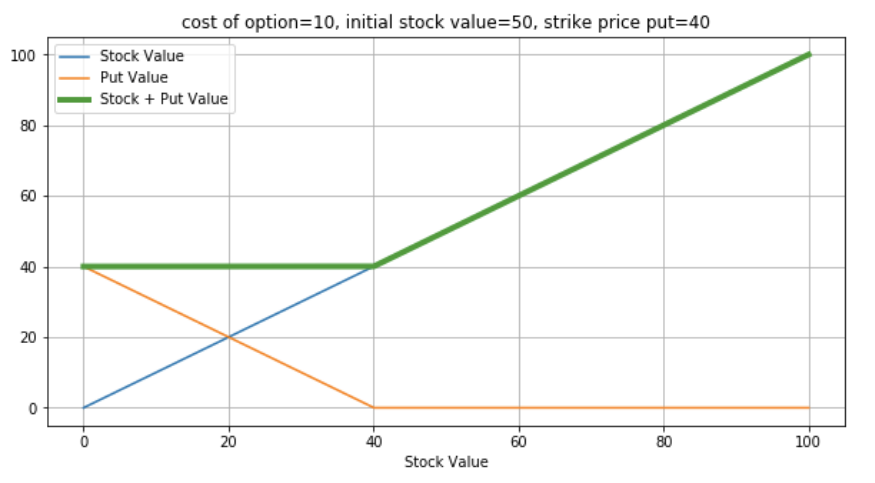
\includegraphics[width=0.8\textwidth]{images/diagrams2.png}
\caption{Stock + Put Option Value Diagram.}
\label{fig:SPValue}
\end{figure}

\begin{figure}[h!]
\centering
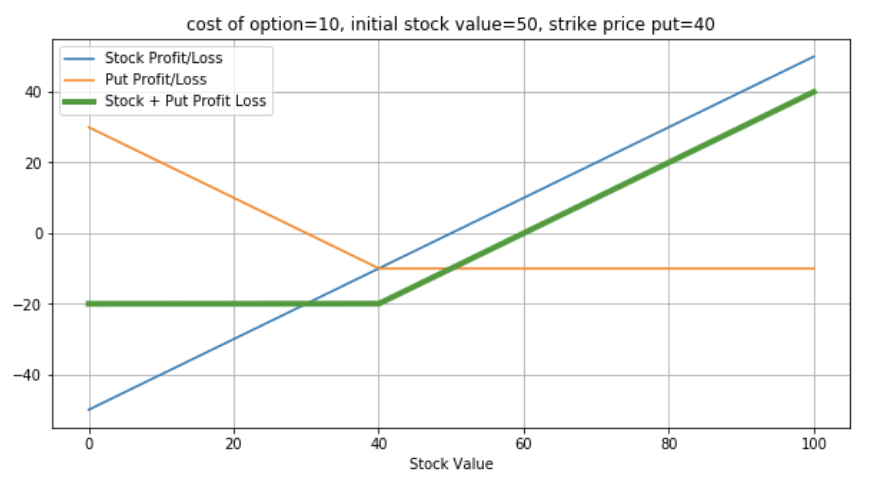
\includegraphics[width=0.8\textwidth]{images/diagrams3.png}
\caption{Stock + Put Option Profit/Loss Diagram.}
\label{fig:SPPL}
\end{figure}

What is the value diagram of a bond? Assuming we are lending money now at $S$ and getting back at maturity a sum $S_1$, regardless of the stock value, the value diagram would be a straight line parallel to the x-axis crossing the y-axis at $S_1$\footnote{What is the profit/loss diagram of a bond and a call???}. An example is shown in Figure~\ref{fig:BCValue}.
By looking at the value diagram, we can see that having a stock and a put is the same as having a bond and a call, in other words: $S + P = B + C$ and this is the so-called put/call parity. If this is not the case, there is an opportunity to make risk-free money (explained later).

\begin{figure}[h!]
\centering
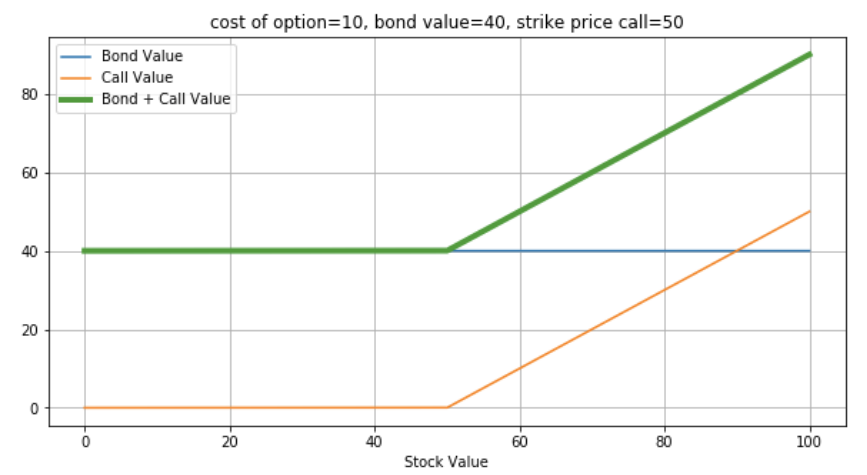
\includegraphics[width=0.8\textwidth]{images/diagrams4.png}
\caption{Bond + Call Option Value Diagram.}
\label{fig:BCValue}
\end{figure}


Owning both a put and a call option allows you to make money if you foresee a big change in value of the stock. Assuming that the P/L diagram is just a down-shift of the value diagram depending on the price of the two options, one makes profit when the stock price increases or decreases more than the price of the two options. This can be easily verified by drawing put and call P/L diagram with the same strike-price (see Figure~\ref{fig:long_straddle}).

\begin{figure}[h!]
\centering
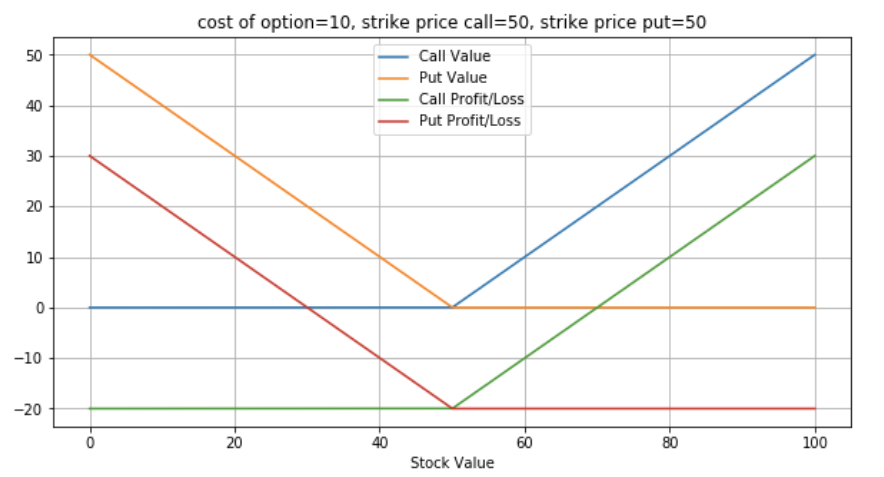
\includegraphics[width=0.8\textwidth]{images/long_straddle.png}
\caption{Long Straddle Diagram.}
\label{fig:long_straddle}
\end{figure}


If you are able to buy a call or a put option is because there is someone willing to give you the right to buy or sell in the future the stock. This person is the option writer and her value and profit/loss diagram is the mirror image ($y' = - y$) of the option holder.

Assume a stock price is $s$, its put option is trading at $p$ for a strike value $P$ and the call option is trading at $c$ for a strike value $C$. Assume also a bond you can buy at $b$ that is worth $B$ at expiry date (the same as the options) and $B = P = C$.
Now, what if $s + p > c + b$? In finance, you always buy low and sell high, so you get the call option and the bond and you sell (short) the stock and you write a put option. By doing this you immediately get money $m = s + p - c - b$. Then, at expiry date you remain with this initial profit and everything else cancels out. Let's see how from a value perspective. If the stock value goes to zero, you don't exercise the call option and it's worthless, you buy the stock at zero to cover the short, you have to buy the stock at price $P$ from the put option you wrote, but you get $B$ from the bond, hence no additional profits, nor losses, only the initial profit $m$. If the stock value goes close to zero, the stock bought with the put option can then be sold, essentially covering the short position. What if the stock price increases instead to $s_1$? You exercise the call option with a strike price $C$ and you get $s_1 - C$, you also have $B$ from the bond and you will have to cover the short by spending $s_1$ which is exactly what you have from the call and the bond,  while the put option is worthless and it won't be exercised by its owner. Similar reasoning can be done if $s + p < c + b$, in which case you buy the stock and a put option, while you write the call and sell the bond, with a profit $m = c + b - s - p$. If the stock goes to zero, you exercise the put option and get $P$, the stock is worthless and the call is not exercised by its owner, but you must pay back your bond of $B=P$. If the stock value goes to $s_1 > P$, you don't exercise the put, you have the stock which is worth $s_1$, you lose $s_1 - C$ from the call option and you pay $B$, again no profits, nor losses.

To better understand put and call options, let's examine Figure~\ref{fig:GEoptions}. Upper-left corner is the current stock price. Call options on the left, put options on the right, in the middle the strike price for both of them. Column \textit{Last} is the last trading price, \textit{Chg} is how much it changed during that day, \textit{Volume} is the number of options traded during that day, \textit{Open interest} is how may open contracts are available in the market. If you sum \textit{Last} and \textit{Strike Price}, you get a bit more than the current stock price because you have the option to buy the stock and make for money in the future, till the expiry date, which is April 2011 in this case (always the third Friday of the month). The longer the validity of the option, the higher the trading price, because you have more opportunity to make money. It is always better not to exercise the option before the expiry date, because you may lose the opportunity to make money. The best solution would be to sell it to someone, charging him this opportunity.

\begin{figure}[h!]
\centering
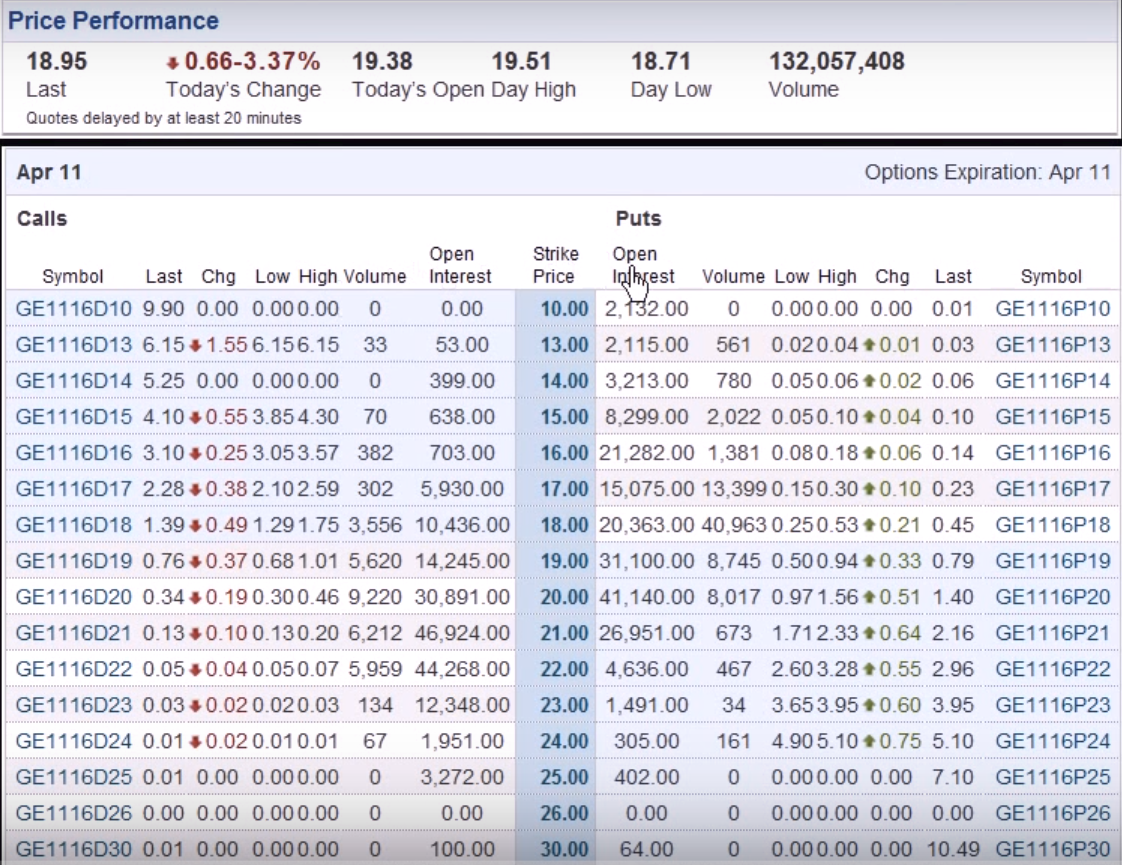
\includegraphics[width=0.8\textwidth]{images/GE_options.png}
\caption{GE call and put options.}
\label{fig:GEoptions}
\end{figure}

When a stock has a very high volatility, it is good to use put or call options as you may exercise them very easily, but their cost will go up consequently.

\section{Forward and futures contracts}
A forward contract is a document in which a seller and a buyer agree upon a certain price of a certain good or service at a specific date in the future. An example is when a farmer wants to sell apples and a food chain wants to buy them but recently the price has been very volatile depending on the good or bad season. Low price is good for the chain, high price is not, so they find an appropriate price.

What if the seller is not able to keep his promises? Or the chain goes bankrupt? What if the farmer wants to change slightly the contract, but another farmer is willing to get the old one? Future contracts are standardized forward contracts, guaranteed by an exchange and may offer more granular options on price and quantity, satisfying multiple sellers and buyers. 

How can an exchange make money out of this? Continuing the example of the farmer and the chain, the exchange will ask a certain price $p$ per Kg of apple to the chain and it will give to the farmer a sum $s < p$. Imagine now that there is another farmer willing to sell apples at a lower price $s' < s$ on a future contract and the exchange will sell this at a price $s' < s$. The aforementioned buyer will be pretty angry now because there is a cheaper option she cannot use and is tempted not to put the money at the end of the contract. To hedge this risk, the exchange asks both parties to set aside a sum, called margin, that the exchange will use in case of price oscillation of the same future contracts in the market. If there is a future contract with a cheaper price per unity of good, the exchange will take the difference from the buyer and give it to the seller. Vice versa, if the price increases the exchange will take money from the seller and put it in the buyer margin. If a margin of a party goes below a certain threshold called maintenance margin, the exchange will ask the party to put money again in its margin and go back to the original margin value. This is a mark-to-market technique because the exchange marks the price of the goods in the future contract depending on its value on the market.

A normal future curve has an increasing trend. On the x-axis we have the time for the contract to expire, and on the y-axis the value of the good. At time $t = 0$, the price is the spot price, while at $t = t'$ the curve is telling you what is the price of the good at which today you agree to buy in the at time $t'$. Of course this curve will not exactly follow the spot price day by day as new events may change the price. For example, if they discover a new application for silver, it's futures price will increase. An inverted curve has instead a decreasing trend and appears in particular occasions. 

\subsection{Contango}
A commodity market (in general metals or long-term investments) is in contango when it is cheaper to buy the commodity now than with a future contract. If you buy gold now, it is usually because you think in the future will value more, but buying it now has some costs: storing it somewhere safe and the cost of cash (you could have invested your money in something else). If you instead enter a future contract, you can use your money for other investments while waiting for the end of the future contract and you don't have the cost of storing.
An alternative and probably more precise definition of contango is when the commodity price agreed today to pay at contract's maturity is higher than the estimated spot price of the commodity at contract's maturity. In general, a severe contango means that the cost of financing and storing a current purchase for sale later is very high, but also that we have a surplus now or we'll have a shortage in the future.
If there is a severe contango situation, you'd buy the commodity now, enter a future contract as seller, store the commodity and sell it at maturity, making money thanks to the cheaper-than-expected costs of having the commodity. If many people start doing this it would increase the price of the commodity at the beginning and decrease it at maturity when more people will sell. This opportunity of making free money will disappear quickly as more people will spot it and eventually the future price will be equal to\footnote{We can think of it as an upper bound.} the spot price plus the cost of storing and financing (borrow money) the commodity.
From Investopedia.com: "Contango is when the futures price is above the expected future spot price. Because the futures price must converge on the expected future spot price, contango implies that futures prices are falling over time as new information brings them into line with the expected future spot price".
\subsection{Backwardation}
Backwardation is instead when the future price of the commodity is lower than the expected spot price in the future. What you should do in this case is to enter a future contract as a buyer and buy a risk-free bond that will pay you at maturity the exact amount of money needed for the future contract. This would be cheaper than buying the commodity now and storing it. Again, as soon as many people spot this opportunity of easy money, the future price will be equal to the spot price of today plus the cost of storing and the risk-free interest rate\footnote{This would be a lower bound.}. The risk-free interest rate and the loan borrowing interest rate play the role of determining the commodity's price: If they are the same rate, the price would be rational, if they are not, there would be arbitrage.
Normal backwardation is desirable for speculators who are "net long" in their positions: they want the futures price to increase.

An important note. When we say that the futures price converges to the spot price by the time we get closer to maturity time, this does not mean that a \$100 future contract will be changed to say \$80. It means that the \$20 from the margin will be sent from the buyer to the seller and the contract looks like a \$80 future, but still \$100 will be paid at maturity.

Contango and normal backwardation are just theories because you cannot be sure about the spot price of a commodity in the future, you just have an estimate. You can see though the phenomenon of contango or backwardation when futures prices are adjusted (decreasing or increasing) to the spot price.

The fair value of a futures contract is the strike price of the future contract at which the buyer is neutral between buying the stock (commodity) in the market now or in the futures market for the next expiry date. Futures markets have much longer trading hours, sometimes also 24 hours. Let's assume that a stock closed at a spot price $S$, and the corresponding fair value (in future strike price) for the next front month was $S + 2$, but now the futures market trades the same stock currently at $S+1$. This means that the spot price should be lower (around $S - 1$ to keep the same gap of 2) and as soon as the stock market will reopen, the stock value will go down as the market will sell the commodity. By having this information, one could think of taking advantage of it, but nowadays there are automated systems that look at these futures contracts and execute high-frequency trading to immediately exploit these opportunities and make money. If instead the futures price is at say $S+5$, the stock value should be higher.

\section{Mortgage-backed securities}
When someone needs a loan to buy a house, she goes to a commercial bank and gets it with some interest rate. This commercial bank will have lots of other customers with their respective loans. What this bank can do to get some immediate cash is to sell these mortgages to an investment bank with some sort of fees. This investment bank usually creates a special purpose entity (SPE) with these mortgages as assets and will try to sell shares of this company to investors hoping to sell the stocks at a higher price than what the SPE spent to buy the mortgages. These stock are called mortgage-backed securities (MBS)

\section{Collateralized debt obligations}
The MBSs can be split in different tranches. One with a lower interest rate but more secure, a mezzanine in the middle and the last is the most junior, the equity with higher interest rate but more risk. These are collateralized debt obligations.

\section{Credit default swaps}
An example to introduce credit default swaps (CDS) is the following. A pension fund, which collects pensions from people can only invest on companies with good ratings. What if it wants to borrow a sum of money $S$ to company A, which has a rating lower than the allowed threshold? The pension fund can pay a small percentage $r_{CDS}$, for example 2\% of the bond from company A with a rate $r_B$, say 10\%, to an insurance company, with a good rating, which will intervene in case of default of the company. So, the pension fund is basically getting a bond with an interest rate $r_E = r_B - r_{CDS} = 8\%$ backed by the insurance company with good ratings, but the bond itself comes from company A which has bad ratings. The insurance company can be any business as long as it has a good rating. The pension fund is buying CDS and the insurance company is selling CDS. The insurance company though is not obliged to put some money aside in case of default from company A, but the rating will change if they don't, in the long run.

Now, if some expert, e.g., a hedge fund, thinks that a company is going to default soon and wants to bet against it, it can buy a CDS without lending the money to the company (it's just a bet between CDS buyer and seller). This means that the hedge fund will pay the annual small percentage of interest rate $r_{CDS}$ to the CDS issuer to cover a sum $S$, as a normal pension fund would do, and if the company defaults, than it would get the sum $S$. The interesting part here is that the CDS buyer can bet on any sum $S$ as long as he can pay $S\cdot r_{CDS}$ every year to the CDS issuer. Of course, the CDS buyer will lose money if the company does not default. The sooner the default, the smaller the costs, the higher the profit.

The risk here is that if company A defaults, the CDS seller may be able to pay money to the buyer of company A's CDS, but what if by doing this, the CDS seller gets its ratings degraded? All the other CDS that were sold by that insurance company are now to be unwound. 
As pointed out also by Warren Buffett, the CDS system is (or at least was) dangerous for the entire financial system because an insurance company is taking bets on amounts of money far larger than what they can insure, without taking the proper countermeasures in case of actual defaults. So, the people, hedge funds for example, who thought to be insured, are now facing risk and people who were hedging on hedge funds are at risk as well.

Another example of CDS buyer is when a special-purpose entity offers CDOs and wants to get some sort of insurance on the senior tranche.

\section{Interest rate swaps}
In general there are two possible ways to decide the interest rate of a loan. The simpler is to fix it at a certain number $r_f$, the other is to keep it variable with time according to another index (e.g., LIBOR). What if someone has a fixed interest rate but would like to have a variable interest rate? And what about the opposite, someone with a variable rate that would like to fix it at a certain rate? The purpose of interest rate swaps is exactly this, to change from fix to variable and vice versa. Alice has a loan with a bank with fixed interest rate $r_f$ and Bob has a variable interest rate $r_v = LIBOR + k$, where $k$ is some non-negative constant. With a interest rate swap, Alice would pay $r_f$ to her bank plus $r_v$ to Bob, while Bob would pay $r_v$ to his bank and $r_f$ to Alice. So, net net they swapped their interests.


\section{Black-Scholes formula}
Given a certain stock price $S$, the exercise price $X$ (strike price) of its call option, its standard deviation of log returns (volatility) $\sigma$, the current risk-free interest rate $r$, the B.S. formula gives us the correct price $C$ of a European call option with a time to expiration $T$.

\begin{equation}
    \label{eq:BSformula}
    C = S \mathcal{N}(\delta_1) - X e^{-r T} \mathcal{N}(\delta_2)
\end{equation}
where:
\begin{equation}
    \delta_1 = \dfrac{\ln{\Big(\dfrac{S}{X}\Big)} + (r + \dfrac{\sigma^2}{2})T}{\sigma \sqrt{T}}
\end{equation}
\begin{equation}
    \delta_2 = \dfrac{\ln{\Big(\dfrac{S}{X}\Big)} + (r - \dfrac{\sigma^2}{2})T}{\sigma \sqrt{T}}
\end{equation}
and $\mathcal{N}(x)$ is the CDF of the normal distribution.
The input values are five: $S, X, T, r$ and $\sigma$. This last value is only the historical volatility of the stock, which is used as an estimation of its future value.
As call options are traded in the market, one can use this formula to get the implied volatility of the stock simply inverting the equation.

\section{Additional notes}

\subsection{Selling put options of bonds}
"For the second day in a row, a put option on the 30-year Treasuries futures contract was heavily sold, a sign of confidence that long-end yields won’t rise much." \citep{yield_inversion}

To me, if a put option is heavily sold, it means that the markets predict the price of the underlying asset will lose value, so that they will be able to sell the asset at the exercise price which is higher than the current strike price. Applying this to the bond market, if what I wrote above is true, they think the prices of US treasuries will be lower, which means higher interest rates. Where am I wrong? The answer is that I misinterpreted the news and what I wrote is a bit misleading. If a put option is heavily sold, the sellers think the underlying asset won't lose value, the buyer does think the asset will lose value.


\chapter{MONEY, BANKING AND CENTRAL BANKS}
\begin{chapquote}{Satoshi Nakamoto, Genesis Block}
``The Times 03/Jan/2009 Chancellor on brink of second bailout for banks.''
\end{chapquote}

\section{Banking and money}
The objective of a bank is to make profit by providing money belonging to people that don't need it immediately to people that instead need it for some purposes.

\subsection{M0, M1 and reserve ratio}
Imagine a world in which there are $N$ coins of gold owned by the people and one bank. These coins are not needed by the people, but there is a guy with a very good idea and wants to start a business that will help society, but he needs a fraction $f$ of $N$. If it's safer for people to store gold in the bank and if the business plan seems reasonable, then the bank will borrow gold from the people with an interest rate of $r_B$ and will lend it to the business man with a higher interest rate $r_L$. If the business succeeds, then the employees will get gold as a salary and they will store it again in the bank. At this point we know that there are still $N$ coins of gold physically, but in fact they are more. They are $N$ from the initial people and $fN$ from the employees. The former value is called \textit{M0}, the second value is called \textit{M1}. This works only if the business really succeeds in its work.

If a person comes to this bank and gives her gold in exchange for cash or a checking account, then she will be able to write checks for payments to other people. A checking account can be opened also for a person who needs a loan from the bank~\footnote{Remember, a loan in this case is an asset for the bank.}. Checking accounts are always liabilities for the bank.

The reserve ratio in this example is the ratio between the amount of gold in the bank and the quantity of gold corresponding to all the checking accounts and cash in the demand liabilities, which is also the ratio $M0/M1$. This ratio cannot be lower than a certain threshold. This percentage indicates what is the percentage of the clients that can come back to the bank and ask for their money at the same time. If more than that percentage suddenly show up, the bank won't be able to provide the liquidity. The smaller the reserve ratio, the better for the bank because it can make profit from all the investment, but as always this comes with risks. A banking system with a reserve ratio different from 1, is called fractional reserve banking

\subsection{Solvency, liquidity and leverage}
Solvency, or being solvent, is when the assets are larger than the demand liabilities―assuming the loans in the assets are good. This means that a bank can pay all the creditors within a certain amount of time. Insolvency happens usually when loans in the assets are not paid back and this results in negative equity for the bank. Keep in mind that a bank can have a checking account for someone, say a company, as a demand liability with a corresponding loan to the same company as an asset. If the company writes checks to other people, but then it's not able to pay back the loan, the bank must have money to pay the check to the people.

The leverage is the ratio between assets and equity. Assuming the bank has only demand liabilities $L$, then the leverage $l$ can be also written as: $l = \dfrac{A}{E} = \dfrac{L+E}{E} = 1 + \dfrac{L}{E}$. With a given leverage of $l$, a bank could bear a loss $pA$ if $pA < E = \dfrac{A}{l}$, which means the higher the leverage, the smaller the losses a bank can afford.
An alternative, but equivalent definition of leverage is the ratio between demand liabilities and equity $l = \dfrac{L}{E}$. 

In the real world there are multiple banks. If these banks have different reserve ratios, things might go wrong. What happens if the bank with the lowest reserve ratio becomes illiquid? People will stop trusting banks and a bank run will happen. It would be better if the bank with the highest reserve ratio lent money to the illiquid one, so as to avoid a bank run that would kill all the banks. 

\subsection{The central bank}
To avoid this problem of liquidity, there exists a central bank which combines this reserve of money. Each bank can have a different reserve ratio and when a bank need cash, more than its current reserve, it can get it from the central reserve. Furthermore, to make people feel more safe, this central bank is linked with the government. This means that the government can raise taxes or issue money and provide them to the creditors. 

In society there is sometimes the need to increase the money supply, for example when there are more people, or more factories and businesses producing wealth. To achieve this, the central bank prints bank notes and the government issues obligations. Citizens then buy obligations from the government hoping to make some money in the future. The central bank finally buys these obligations from the citizens\footnote{This is an open market operation, so the seller of the obligation does not know the buyer (the central bank, in this case).}, which can in turn put money back into their bank accounts. The net result is that there is now more money in the system.

In theory, a central bank has no equity and the liabilities it has with other banks have no interests. The assets are composed of cash and obligations (treasury bonds for example) that generate profit. In practice, a positive equity goes to the government and a negative equity means the government will provide money.

\subsection{Target rate}
If two banks have different reserve ratios and bank $A$ needs some cash for one day (overnight) from bank $B$ with higher reserve ratio, $A$ will ask for a loan and $B$ will give it a certain interest rate. The central bank, as already explained, can print money and then buy obligations from people than in turn will put their money into banks. This will result in banks having more money, so $A$ will need less money and will be willing to pay a lower interest rate and $B$ as well will be willing to offer a lower interest rate. The target rate (fed fund rate) is the rate at which the central bank wants other banks to lend money to each other\footnote{It is on an annual basis, then if money is needed for just one day, it is just a fraction of it.}. The central bank can increase it, as said before, but also decrease it by buying obligations (short-term treasury bonds that are less risky). The reason why they use this parameter to decide on monetary policy is that its value is easily accessible, just ask a bank for a loan. Instead, measuring the value of $M0$ or $M1$ is much more difficult and not real-time. 

The central bank tries to manage the target rate, which is the interest rate at which banks lend money to each other, but by increasing the money supply the cost of lending will decrease, so also companies and people will get cheaper loans.

Another reason why dealing with interest rates instead of amount of money available is that it allows to select businesses in a better way. What does this mean? Imagine we have 4 different companies, each with a project to finance and in need of the same amount of money $S$ but they are willing to pay different interest rates for their businesses: Good business plans will be willing to pay higher interest rates. If we focus on interest rates and we tune them depending on the period (growth or not), we can set a sort of threshold on how good a business should be or, in other words, how much wealth it should be able to generate. If we focus on available money instead we would always finance the best businesses and this is a problem in periods when there are no good projects to invest on. 

A repurchase agreement is when party $A$ gets a loan from party $B$ covered by some assets belonging to $A$ and also a repurchase agreement is given to $B$. This agreement says that $A$ will buy back its assets from $B$ but at a higher price (the loan + interests).

\subsection{The discount rate}
When a bank has no more liquidity and it's not able to get loans from other banks at the fed funds rate (target) because they don't trust it, then it's last option is to ask for a loan to the federal reserve but with a higher rate, the discount rate. The money from the central bank is printed, not taken from the previous assets.

When a person puts money in the bank, she can be told she can withdraw the money at any time or that she can withdraw only 10\% of the money at any time and the rest later. In the second case, one should ask for interests because the bank is using her money to make profit.

\subsection{Federal Deposit Insurance Corporation}
With fractional reserve banking, one bad bank (with money invested in bad loans) may lead to big problems for every other bank. Moreover, A central bank can help banks in this situation, but it must be able to differentiate which bank is good and which cannot pay its debt (insolvent). In case the central bank is not willing to lend money to a bad bank, there is a second option. It's called Federal Deposit Insurance Corporation. The idea is that each bank pays a small percentage to the FDIC, a sort of insurance that in case of a bank has lack of liquidity, has made bad investments or is going bankrupt, the FDIC provides liquidity to the banks avoiding bank run. This percentage is usually lower than the interest rate of the loans provided to the people, so a bank is willing to use this insurance to be safer and also to lower interest rates to its clients. When there is a good period for the economy, the percentage paid to the FDIC is low, but when things go bad, it increases. It's interesting to note that this insurance does not have the same properties of normal insurances. Here, a bad event is usually correlated to other bad events because the financial system is connected. Instead, car accidents are usually uncorrelated and they spread throughout the time. A high interest rate is always seen as a risky investment, but if backed by the FDIC, it is much more secure. If a bank is insured by the FDIC, it is encouraged to make riskier investments, offering higher interest rates. 

\subsection{You don't need a fancy MBA}
Venture capitalists, private equity and hedge funds provide basically the same service of banks: get money from people who do not now how to invest and use it to finance some businesses. The big difference is that they do not operate on fractional reserve banking. They may say upfront that some part of the money is locked up for some years and some part is on demand (liquid), but there is absolutely no problem like bank run. Moreover, they add value to society investing in businesses and startups. Now the critic part. With fractional reserve banking a bank takes money from a normal person claiming that her money is always available―as long as a fraction of the population does not withdraw all their money. Since it's money almost "always available", she does not get a high interest on that money, but, by being insured by the FDIC, the bank can invest on much more risky companies with much higher interest rates or on long-term treasury bonds and make more profit\footnote{Sal's critic: "Anyone can do this. You don't need a fancy MBA to figure this out. This doesn't add any true value to society."}. All of this because of the FDIC. Note that when the FDIC has no more money, the government raises taxes on citizens. Is this even capitalism? Where is the competition? Where is the innovation? The most successful banks will have riskier investments and if everything goes wrong, there is the FDIC to cover the losses\footnote{"The banks are holding us at gun point and threatening to take us all down with them if we don't bail them out. They argue that if they go down the economy tanks with them since there will be nobody to give out loans when they're gone. Unfortunately, this is true to an extent because the government allowed them all to consolidate to the point that if a single one of these big banks failed there would be enough paperwork to send the economy to a screeching halt." Comment from FishHead}\footnote{"What the FDIC's intervention leads to though, is to reduce the risk to depositors to 0 (by taking onto itself any catastrophic loss, like what happened in the mortgage crisis). The fact that the depositors have 0 risk to their money means that they accept to give it to the bank to very low interest rate (like Bank of America that was (and might still be, not sure) giving 0.1\% interest rate on the money to depositors). If there was a risk to give money to the bank, because it was not FDIC insured, the only way people would put it there is if there was a decent amount of interest accumulating." Comment by Patccmoi}.

Another useful parameter is the LIBOR, London Inter-bank Offered Rate, an average rate at which banks lend money between themselves.

\section{Quantitative easing}

So far, we know that the central bank can buy short-term treasury bonds to lower the fed fund rate (target). This is injecting money to the system and lowering the yield curve where the maturity time is short (few days). By keep buying bonds, this rate can reach zero. What if this is not enough to stimulate the economy? The central bank can start buying long-term bonds, lowering again the yield curve. It can also buy mortgage-backed loans, or corporate debt to make the market more liquid. This is quantitative easing. 

In quantitative easing generally, the central bank is trying to lower the yield curve, first with treasury bonds. The hope is that by doing this, also other rates get lower, such as mortgage loans and corporate debt. If this does not happen, it is dangerous because the spread (difference) between treasury bonds and other types of debt increases. In 2009 Bernanke tried to avoid this danger by buying exactly these assets to increase demand and lower interest rates in these specific markets and he called this "credit easing". Japan instead did quantitative easing just for the sake of printing money without paying much attention on where the money was going.

\section{2008 bank bailout}

\subsection{Mark-to-model or mark-to-market writedown}
As already seen in section \ref{Corporate metrics and valuation}, a company provides a book value for its equity, based on its analysis of assets and liabilities. This may differ from the value of the market. This happens usually because the value of some assets are valued differently by the company and the market. If the book value and the market value differ a lot, the company can do two things: mark-to-model or mark-to-market writedown. In the first case, the company asks some special analysts to create fancy models and valuate their critical assets (mostly derivatives and other toxic assets) leading to a correction, or writedown, of their total assets' value. In the second case, the company simply looks at the price of those critical assets in the open market. In the former case, the assets value may be biased in favor of the company, in the latter it may be biased against the company and in favor of the skeptics because in the open market people sell and buy driven by their feelings (fear, excitement).

\subsection{Bank bailout example}
A typical scenario of bank bailout is the following. A bank has assets like cash, treasury bonds, AAA corporate bonds, and derivatives and has liabilities such as loans to different entities. Usually this loans are interest-only meaning that during the loan only the interest gets paid while the loan is paid at once at the end\footnote{This is done to take advantage of tax-deductible income as already seen in section \ref{mortgages} and \ref{Personal taxes}.} and what happens is that the loan will be renewed at its expiry date and it remains interest-only. The problem arises when the lender of the loan does not want to renew it because for example the debtor owns toxic assets (assets that are worthless or difficult to sell). Now the debtor―the bank in our case―has to pay back the entire loan and to do get money immediately it starts selling treasury bonds. The same process repeats when other loans mature and if the bank does not have any more treasury bonds, then it can sell AAA corporate bonds, which are still easy to sell, but probably not at the expected price, so the equity starts shrinking. The critical step is reached when the bank has to pay back a loan but the only remaining assets are cash and toxic derivatives or the like. Here, the bank cannot use cash because they need it for the daily operations, so it tries to sell the derivatives, but they have to be sold at price $X$ such that it allows the bank to pay back all the debt it has, otherwise it would be useless and the bank would go bankrupt anyway. If the market is not willing to buy these assets at price $X$, then there are two choices―at least.

One option for the bank is to issue shares and find an investor―usually a foreign entity with the currency used by the bank or a sovereign wealth fund―willing to buy them such that the bank can then pay back the last loan or loans. Of course, the losers here are the shareholders because the equity decreased a lot and new investors join. At this point, the bank is left with some cash, toxic assets\footnote{The bank hopes they will become good investments in the future.}, no liabilities and equity, so the bank is de-leveraged and it has been bailed out.

A second option is bankruptcy (see section \ref{Life of a company}). Here the company can completely shut down after the liquidation of all its assets or can still operate but the previous shareholders are wiped out and the last creditor of the company becomes the new single shareholder with new shares and only liquid assets (toxic ones are sold, regardless of their value).

\subsection{The moral hazard and the incentive to create bubbles}
Imagine a scenario in which a lot of banks have toxic derivatives as assets or CDOs (Collateralized Debt Obligations) and they owe money to each other in form of loans. If one bank discovers that its toxic assets are worth less than the equity, as in the case seen above, then this bank becomes insolvent and this lead to a chain reaction in the whole banking system. If a creditor bank now loses money because of this insolvent bank, on top of its other risky investments, it too will face difficulties or bankruptcy. More generally the problem is not related to only one risky asset, rather all of them deteriorate and are worth less.

To avoid this problem, the central bank can decide to buy more risky derivatives and CDOs from the banks, hoping that this money will enter the system and start circulating, but also to create demand for these assets with a reverse auction\footnote{In this case, a reverse auction means that the central bank is willing to buy toxic assets from the lowest (cheaper) bidder.}\footnote{Sal is skeptical about this point. If there were people willing to buy these toxic assets, they would have already bought them, without waiting for an artificial demand created by the central bank. Also, if a bank is selling these toxic assets all the other banks will stay away from this bank because they know its a risky bank}. In 2008 though, this did not quite happen because banks were so afraid (their toxic assets were worthless and that they weren't able to pay back their loans) that they did not spend this money, holding it tight for loans due in the future.

When the central bank buys these toxic assets, it should not buy them at fire-sale price (the price of a panicked marked, so extremely discounted prices), but rather at a price that allows the banks to keep a non-negative equity. By doing this, though, the central bank is literally writing a check to the shareholders and to the creditors of the banks at risk, the very people to blame for the problem. The counterargument is that if the central bank does not follow this path, the entire economy will collapse. So hoping that banks fail and go bankrupt may be a good punishment for the bad investments and misbehavior of the bankers, but on the other side there are real businesses and companies that will lose their money because of this event and all the system, not only the banking one, will suffer. 
The deeper problem, or moral hazard, is that when times are good bankers gets a lot of money, bonuses and so on, but when times are bad they can rely on the government and the central bank to cover the losses. This is definitely an incentive to keep creating bubbles and keep taking huge risks.

As explained above, the central bank can print money and buy toxic assets from a bank, but it can also decide to buy new stocks from the bank so that the current share holders are no longer the majority and the bank can pay its debt. By doing so, though, the central bank is helping the bad investors which lent money to the bank. If the central bank is really worried about the real economy and does not care about saving banks because they will come back anyway in few years―hopefully more conscious and with proper risk measures―it should create a fund that will pay back the loans to businesses and people that would have otherwise lost their money they kept in the banks.

\subsection{Worthless CDOs}
But how is it possible that CDOs are worth nothing? Let's see an example. Assume there is a special-purpose entity which lends money in form of mortgage loans, say $N$ loans, to people for a total sum $S$. Of course, to lend money this entity must raise money first. To do this, it splits the sum $S$ into $n$ tranches so that the first one has an interest rate $r_1$, the second one has an interest rate $r_2$ and so on until $r_n$, with $r_1 < r_2 < ... < r_n$, meaning that the first tranche is the least profitable, but it has the highest seniority\footnote{It will be paid first in case of bankruptcy} and the last one is the most profitable, but very risky. Now, even if one single mortgage loan is not paid back to this special-purpose entity, there will be at least one investor that will lose money. The higher the number of unpaid loans, the higher the number of investors that will lose money.

\subsection{Merrill Lynch and the Loan Star Funds' affiliate}
At the end of June 2008, Merrill Lynch had to write down some of its assets from \$30.6 billion to \$11.1 billion. These assets were super senior ABS (Assets-Backed Securities) CDOs. On July 28th, Merrill Lynch agreed to sell these CDOs to an affiliate of Lone Star Funds, a private equity, at a price of \$6.7 billion. This affiliate was financed for this investment by Merrill Lynch itself for 75\% of the total amount, meaning that the affiliate―financed by Lone Star Funds―put \$1.7 billion and got \$5 billion as a loan. In case of insolvency, both parties agreed that the affiliate will not lose more than \$1.7 billion. Say that three months after July, the value set by the market was \$10 billion, then of course Lone Star would profit by \$3.3 billion by selling, and Merrill Lynch could get back their \$5 Billion loan. The fact is that this scenario was quite unlikely to happen, but Merrill Lynch was able to artificially create demand for the CDOs and avoid writing them down immediately and the affiliate was able to get the CDOs paying 6\% of their original value (\$1.7B instead of \$30B).

\section{Geithner plan}
To save the banks in the financial crisis in 2008, the federal reserve came up with a plan where private investors and the central bank team up to create a unique entity. In this entity, the private investors―expert traders that know how to value stocks and bonds―are the shareholders together with the treasury. The private investors contribute a small percentage to the initial assets and the rest is financed with a loan by the fed. The purpose of this entity is to fix a price for the toxic assets of the banks and buy them. If these assets turn out to be non-toxic then the private investors will make money and the loan will be paid back to the fed. If instead these assets are worthless, then the private investors will lose a small amount of money, while the fed will lose more (a fraction of or the whole loan). 

It is interesting to note that nothing can seriously prevent the bank itself to be the private investor in this new entity. This can lead to an overprice of the toxic asset and the bank will face much smaller losses. A possible scenario is the following. The bank with toxic assets starts selling CDSs on those assets with very low interest rates, which means a very cheap insurance on a bank's default. Then, a hedge fund or, more likely, the shareholders of the bank with toxic assets will buy these cheap CDOs to edge their losses in case these assets turn out to be worthless, but they also put money into the special entity with the central bank to save the banks. Now, in case these toxic assets turn out to be good assets, the hedge fund makes money because it has a share in this entity, but in the opposite scenario thanks to the CDSs they don't lose money.

As explained so far, this plan is very much like a put option of the toxic asset. Let's see. Assume that the initial value of this toxic stock was $I$ and the hedge fund was ready to invest the same amount of money on the stock, but it had two possible alternatives, joining the Geithner plan or the put option plus the stock. In the first case, assume the hedge fund is investing a sum $S$ in this special entity, with $S = r \cdot I$ and $r = 15\%$, meaning that $I-S$ is put aside. The Treasury will match this sum and the entity will have an equity $E = 2S$. The central bank then puts a sum of money $L$, so that the banks are able to cover their debt and the entity is capitalized with a total sum $T$. Let's also assume this special entity now buys $N$ stocks for a total price of exactly $T = N \cdot I$. Now, if the stock value in the future $V$ will be such that $NV \leq L$, the hedge fund and the treasury make no profit, but the hedge fund remains with the initial sum $I-S$ that it put aside. If the stock value will be such that $NV > L$, the hedge fund's profit is $P = \dfrac{NV - L}{2}$ but it also has the initial sum $I-S$ that it put aside. The equivalence is shown in Figure \ref{fig:GPlan_HF}.
\begin{figure}[h!]
\centering
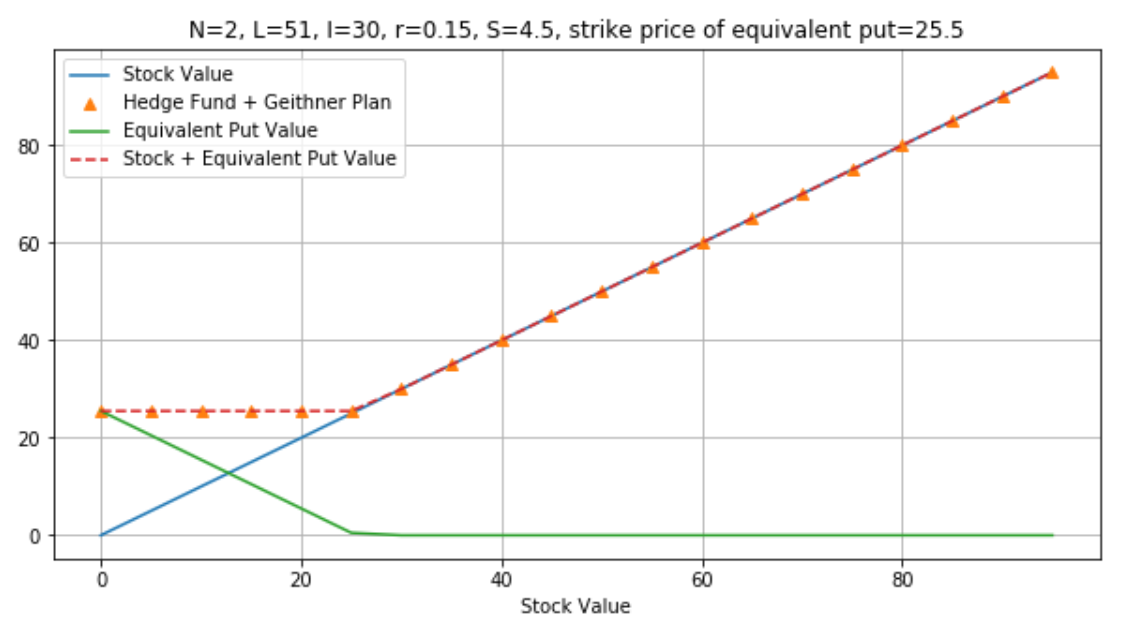
\includegraphics[width=0.8\textwidth]{images/GPlan_HF.png}
\caption{Comparison of the value diagram for a put+stock and the possible Geithner plan exploit.}
\label{fig:GPlan_HF}
\end{figure}
That being said, we can conclude that, to a rational investor, joining the Geithner plan or buying a stock and the put option is equivalent. The second scenario means that the investor should buy the stock at a value $I$ and the put option at a certain price $p$ (which can be computed using the Black-Scholes formula). With the numbers presented in Figure \ref{fig:GPlan_HF}, a reasonable value would be $p = 20$. This means that the investor is willing to put at most $50$ to join the plan. The problem is that this sum from the private investors was not enough to cover the debt of the banks. The banks themselves could form other entities to join the plan as already mentioned.

A possible solution proposed by Sal is that the toxic assets are put into another new company with toxic assets only and then it starts selling shares to the open market (e.g., NYSE). This new company should be transparent, explaining what are the assets so that any investor can easily decide whether to buy or not. Otherwise these assets would remain obscure and hard to buy for the majority of the investors, reducing the demand and decreasing their price. If the new shares are worthless, then the bank will fail, but at least it will happen in a transparent way and probably with lower likelihood.

\section{Foreign exchange and trade}
Imagine a simplified scenario where there are 2 people, Alice and Bob, willing to exchange RMB with USD and one person, Chen, willing to do the opposite exchange. Both Alice and Bob have 100 RMB and Chen has 100 USD only. Chen decides to put part of his money to the open market to be exchanged in USD. As soon as Alice notices it, she accepts to exchange all her RMB into USD at the rate proposed by Chen: $1 RMB = 1 USD$. Chen understands that there is quite a lot of demand for the currency he has, given that Alice accepted immediately, so he decides to change the rate for the remaining part of his currency: $1 RMB = 2 USD$. Bob has still his 100 RMB and given the fact that last time he wasn't able to exchange the sum because Alice was faster, now accepts the new and worse rate proposed by Chen. In this scenario, the price of USD went down compared to RMB and the price of RMB went up compared to USD, meaning that it is now a bit more difficult to buy RMB with USD (you need more USD to get one RMB) and it is easier to get USD with RMB (you need less RMB to get one USD). Notice that there is no relationship between the fact that the price of RMB as gone up compared to USD and the ratio between the amount of RMB available and the amount of USD available. It all depends on the offer and the demand.

Imagine now that Chen needs to sell $n$ units of his product at $X$ RMB each in the USA, where Alice lives, in order to cover the costs and make some profit. Alice instead needs to sell $m$ units of her product at $Y$ USD each in China, where Chen lives. If now they have to exchange their currencies with a rate $1 RMB = 1 USD$, Alice gets 100 USD and Chen gets 100 RMB. What if the next year, there is also Bob involved in the market? As seen above, Chen will change the exchange rate to $1 RMB = 2 USD$. This means that Chen will now sell his product in the USA for double of the previous USD price (but at the same RMB price if it would be in China), while Alice will sell in China for half of the RMB price (but at the same USD price if it would be in the USA). Doubling the price leads roughly to half of the units of product sold and vice versa with halving the price. This results in a balance between how much wealth (number of products times value of each product) is shipped in the USA and how much is shipped to China.

The main takeaway is that when there is more demand for currency A than its supply, its "price" compared to currency B will go up (more people want to have A but they have B). From a trade perspective this means that people from the country with B as currency can lower prices of products sold in the country with A, and vice versa, people from country with A and selling in the country with B should increase the prices, which will reduce the number of products sold. The trade imbalance will also decrease, eventually becoming balanced.

Assume we have an exchange rate $e = .87EUR/GBP$, this means that if we have 100EUR and we want to know the value in GBP we multiply 100EUR by .87 and we get 87GBP, simple. In general, with an exchange rate $e = r*A/B$, to go from a sum in A to a sum in B we multiply the sum in A by $r$. 

If $r$ decreases, A is getting weaker compared to B and it will be more expensive for people with currency A to buy products sold in currency B, which means more coins of A are needed to get one coin of B. This is bad for the consumers, but maybe not so bad from a trade balance point of view, because the country with A will be able to sell their products at lower prices in other countries.

If instead $r$ increases, A is getting stronger compared to B and it will be cheaper for people with currency A to buy products sold in currency B. This is good for the consumers, but maybe not so good from a trade balance point of view, because foreign countries will be able to sell their products at lower prices in the country with a stronger currency.

\subsection{Carry trade}
A carry trade is a situation where a currency A can be borrowed at interest rate $r_A$ and a currency B can be borrowed at $r_B > r_A$ with an exchange rate of $1 A = c B$, and this holds for a long period during which an investor can borrow a sum $S_A$ of A, convert it into a sum $S_B = S_A \cdot c$ of B, lend $S_B$, get $S_B' = S_B \cdot r_B$ in interest and convert back to A to get $S_A' = \dfrac{S_B'}{c} = \dfrac{S_B \cdot r_B}{c} = \dfrac{S_A \cdot c \cdot r_B}{c} = S_A \cdot r_B > S_A \cdot r_A$, making a profit of $P = S_A(r_B-r_A)$. This is free money, but as soon as people will spot this opportunity, we should have $r_A$ and $r_B$ converging to the same value.

\section{Chinese currency and U.S. debt}

\subsection{Pegging the yuan}
What the Chinese government and the Chinese central bank did was to keep printing yuan and trying to convert it into dollar to keep the exchange rate fixed, or pegged (e.g., $10 RMB = 1 USD$) so that for Americans it was always cheap to buy Chinese products. Printing yuan of course means depreciating its value, but on the other side, China was able to produce, sell and grow thanks to Americans buying their products. Chinese inflation is slowed down by a corresponding Chinese growth\footnote{We give China pieces of paper, they give us stuff we want. Does that sound like such a bad deal? - Andrew M.}. At the same time though, the American industries produce much less. 

Once the yuan is printed, the Chinese exchanges it with the dollar in the market. This big sum of dollars in cash are then used to buy safe and liquid assets: US treasury bonds. This leads to lower interest rates as there are more clients willing to get the bond and lower borrowing costs for the government, which means the government could lower taxes or spend more. Note that a central bank (the federal reserve in this case) can regulate only short-term interest rates and not long-term bonds. The net result is more cash in the American pockets, but it's not debt-free cash, it is financed by Chinese yuan.

By printing yuan, China can have an export-led growth and sooner or later, the Chinese will be able to buy products previously inaccessible to them, e.g., manufacturing products (washing machines) and the Americans will lose some low-price markets but will be able to focus on knowledge-based markets and have lower prices. As soon as the Chinese central bank stops printing yuan, the borrowing cost of a loan in USD will be higher and the exchange rate will change so that the prices will not be so low as before.

The Chinese central bank can also decide to buy other assets other than US treasuries, like UK bonds. This will make the GBP worth less compared to USD and to avoid this GBP appreciation, the British central bank would print GBP and buy US treasuries.

Just to give some real numbers, from November 2009 to November 2010, the Chinese central bank reports that the M1 value increased by roughly \$700 billion and around \$422 billion are used in foreign assets. This is again to keep the yuan cheap outside China.

What if the PBOC (People's Bank Of China) stops printing yuan? The yuan will become more expensive, stronger and less Chinese goods will be sold outside China, inflation will decrease and economy will slow down. India or other countries with cheap labor may take the lead in manufacturing sectors. The trade imbalance between China and other countries will decrease. The the interest rates in the US will increase as there is less demand of US bonds. Chinese imports to the US will become more expensive.

\section{2011-2012 Greek debt crisis}

\subsection{The problem}
From 2003 to 2012, the debt-to-GDP ratio of Greece went from 97.4\% to 198.2\% meaning that the Greek debt became twice as much as what the country was able to produce. From 2007 to 2012, the taxes payed by the Greek population were around 40\% of the GDP, while the public expenditures where around 50\% of the GDP, clearly not a good sign for their debt. This led also to higher interest rates for the Greek bonds as people started being suspicious about the Greek government's ability to pay back the debts. 

\subsection{No obvious solution}
One first thought might be to reduce the expenditures and increase taxes, but obviously this is not something a politician would easily do as he would lose consensus. The additional problem was that the GDP growth was negative during that period meaning that the country was in recession and implementing measures of austerity while recession is not a good move because it will slow down the economy, public revenues (taxes) will decrease and interest rates will increase. The solution here is not obvious, but what happened was that Greece received financial help from the EU and implemented at the same time austerity measures, but it did not lead immediately to economic improvements.

A bad idea would be to simply default on the debt. In this case the Greek government would not pay back the investors, but by doing so, all the investors will stop lending money and the state will not have money for pensions for example. It would be a drastic shut down of the government. This is not a good solution.

Being Greece part of the Euro-zone, the debt it was obtaining was pretty cheap thanks to the euro. Another hypothetical alternative, if Greece was not part of the Euro-zone, was to print more drachma, buy government bonds to finance the economy, increase inflation which might help to exit the recession. What's interesting in this possible solution is the following. Imagine Greece had a GDP of $\delta\rho$100B, obligations for $\delta\rho$10B, and a total debt of $\delta\rho$150B. Then in few years, the prices of the goods double thanks to the printed drachma by the Greek central bank. If the number goods and services produced in this period remain constant, but their prices double, the GDP (not adjusted to inflation) will be $\delta\rho$200B, while the obligations and the debt will not change. This is of course something bad because you devalue the state currency, but it would not be a political suicide compared to the previous scenarios. This of course might entail other problems like a spiral inflation.

It's important to know that if the Greek government has obligations and debt in euro and decides to go back to the drachma and pay those obligations with the new currency, it is considered default. In this case, though, the Greek people can go on with their lives using the drachma. Nevertheless, before this can happen, Greece has to declare a bank holiday during which the euros on the bank accounts are converted into drachma and after that the drachma will be publicly exchanged in the market, and will with high likelihood lose its value. Being aware of this scenario, the Greek people will go to their banks and withdraw all their euros, as they know they'll lose buying power otherwise. Run on banks will cause major damages because of the fractional reserve banking.

On the other side, bailing out Greece will be seen by German taxpayers as a very bad and immoral move because they'll see their money rewarding mismanagement of the Greek politicians, while instead they should be punished. The counterargument is that people are already suffering in Greece, so maybe a moral point should not be raised here. The bigger problem is that Greece is not the only country in a bad situation in Europe, so if Greece leaves the Euro-zone, investors will be more suspicious about all the other risky countries.

\section{Additional notes}

\subsection{History of the fed funds rate}
The fed funds rate is raised to fight high inflation, and lowered to fight deflation. 

The Federal Reserve prefers to keep the fed funds rate between 2 and 5 percent. It's the sweet spot that maintains a healthy economy. That's where the nation's gross domestic product grows between 2 percent and 3 percent annually. It has a natural unemployment rate between 4.5 percent and 5.0 percent. Price increases remain below the Fed's inflation target of a 2 percent core inflation rate.

In 1973, inflation tripled, from 3.9 percent to 9.6 percent. The Fed only doubled interest rates from 5.75 to a high of 11 points. Inflation continued to remain in the double-digits through all of 1974, lasting until April 1975. The Fed kept raising the fed funds rate to a peak of 13 in July 1974, and then dramatically lowered the rate, reaching 7.5 by January 1975. These sudden changes, known as stop-go monetary policy, confused businesses.

The all-time low was 0.25 percent. That's effectively zero. The Fed lowered it to this level on December 17, 2008, the 10th rate cut in a little over a year. It didn't raise rates until December 2015. Before this, the lowest fed funds rate was 1.0 percent in 2003, to combat the 2001 recession. At the time, there were fears that the economy was drifting towards deflation \citep{target_rate_history}.

Increased interest rates 2004-06 had a significant impact on US housing market. Higher mortgage costs led to a rise in mortgage defaults – exacerbated by a high number of sub-prime mortgages in the housing bubble. In this case, higher interest rates were a significant factor in bursting the housing bubble and causing the subsequent credit crunch.

%%%%%%%
March 2000, stock market declines, but the Fed raises target rate to 6.5 percent
March 2001, recession begins and the Fed lowers target rate gradually till summer 2003 to 1 percent.
March 2005, higher target rate around 3 percent creates doubts in housing market and risk of defaults for many sub-prime loans.
March 2006, higher target rate around 5 percent to cool housing bubble. First defaults appear.
March 2008, Bear Stearns, Lehman Brothers and AIG bailouts. Lower target rate to stimulate economy.
End 2008, target rate is 0.25 percent.
Till 2017, target rate below 1 percent to stabilize growth.
March 2017, target rate start to increase slowly
March 2018, target rate at 1.75 percent.

\begin{figure}
\makebox[\textwidth][c]{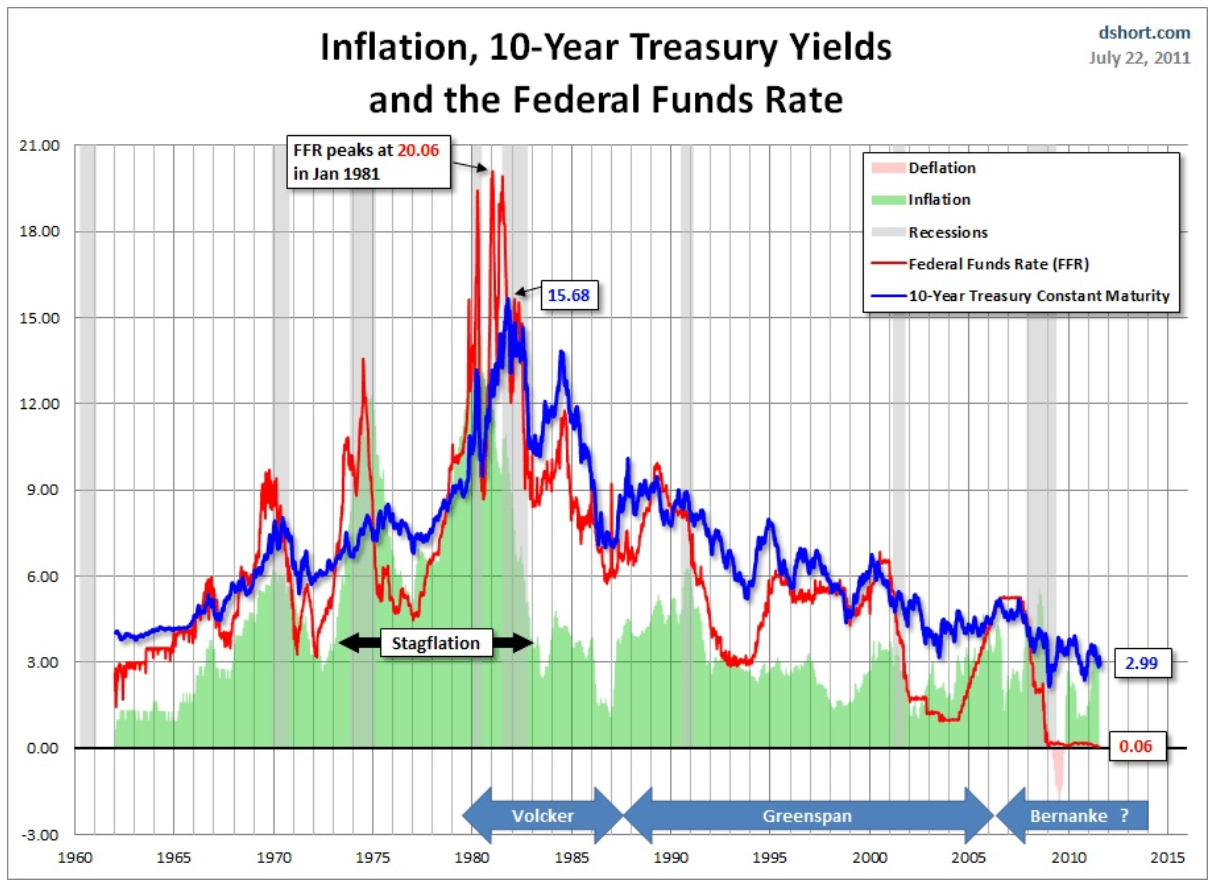
\includegraphics[width=1.1\textwidth]{images/ffr_inflation.png}}
    \caption{US inflation and target rate. }
    \label{fig:cpi_ffr}
\end{figure}

Trying to push rates negative might lead to mass withdrawals of money from banks. That would worsen a financial crisis, and ultimately impose a huge efficiency cost on the economy through the collapse of convenient electronic payments system. Worst of all, once we completed the awkward transition to a cash economy, interest rates would still effectively be stuck at zero — cash pays neither positive nor negative interest — so nothing would be accomplished.

% https://www.vox.com/cards/fed_vs_crisis/
Quantitative easing is often regarded as a form of "printing money" but the Fed doesn't literally print anything. Paper money is printed by the Bureau of Printing and Engraving so that people who want to take money out of their bank accounts can get their hands on cash. But most money is electronic. And, yes, quantitative easing involves the Fed making new money. It then uses that money to buy bonds, injecting extra money into the banking system. The money supply used to increase at a slow but steady pace, but during the 2007 financial crisis, it has instead shot up in several large irregular spurts associated with different rounds of QE. 

What makes it quantitative is that when the Fed does QE it specifies a dollar quantity of assets that it wants to buy. An alternative approach (call it qualitative easing, if you like) would be for the Fed to target a specific outcome it wants to see — conventional mortgage rates below X percent or whatever — and then commit to buying however many assets it takes to create that outcome.

Did all this QE create tons of inflation? No. Inflation was very low during Ben Bernanke's tenure in office. One reason for that is that even though lots of money has been created, much of it is simply parked at the Fed. Banks are required to hold reserves — that is, money that they don't lend out — as a regulatory matter. But lately they've been holding lots of extra reserve money. This stockpiling of excess reserves at the Fed may have happened in part because the Fed now pays interest on them to the banks. Paying interest on excess reserves could be a useful way for the Fed to in effect suck money out of the economy if it becomes worried about inflation in the future. No investment on Earth is safer for banks than parking money at the Fed, so the higher you make that interest rate the more money banks will park. Money that is parked is not being loaned out and spent. So by inducing banks to park their money, the Fed can put the breaks on the economy and stop inflation. 

Another line of criticism, associated with Paul Krugman's 1998 analysis of the Japanese economy, says that the real problem is something else. The Fed wants to reassure people that it has the ability to fight a potential future outbreak of inflation. But QE would be more potent if people were in fact afraid of a potential future outbreak of inflation. People worried that their money may lose value in the near future are more likely to run out and trade that cash for cars or refrigerators or houses and spur economic activity.
\chapter{CURRENT ECONOMICS}
\begin{chapquote}{Giuliano Amato}
``The treaty clause that triggers exit from the European Union was not actually designed to be used.''
\end{chapquote}

As the quote above suggests, this chapter was not designed to be used because the topics presented in the videos are already explained in the previous chapters. They are the "Housing price conundrum", the "Credit crisis" with MBSs, CDOs and so on, the "Paulson bailout". There are new topics, though, about the European Union and the unemployment, but they won't be reported here for now.

I'll use this chapter to keep track and to explain---to me and to the reader---what is happening right now (from April 2018) in finance and economics.

\section{Yield curve: flattening or inversion?}
Sources: \citep{yield_inversion}

\hspace*{-1cm}
\begin{figure}
\makebox[\textwidth][c]{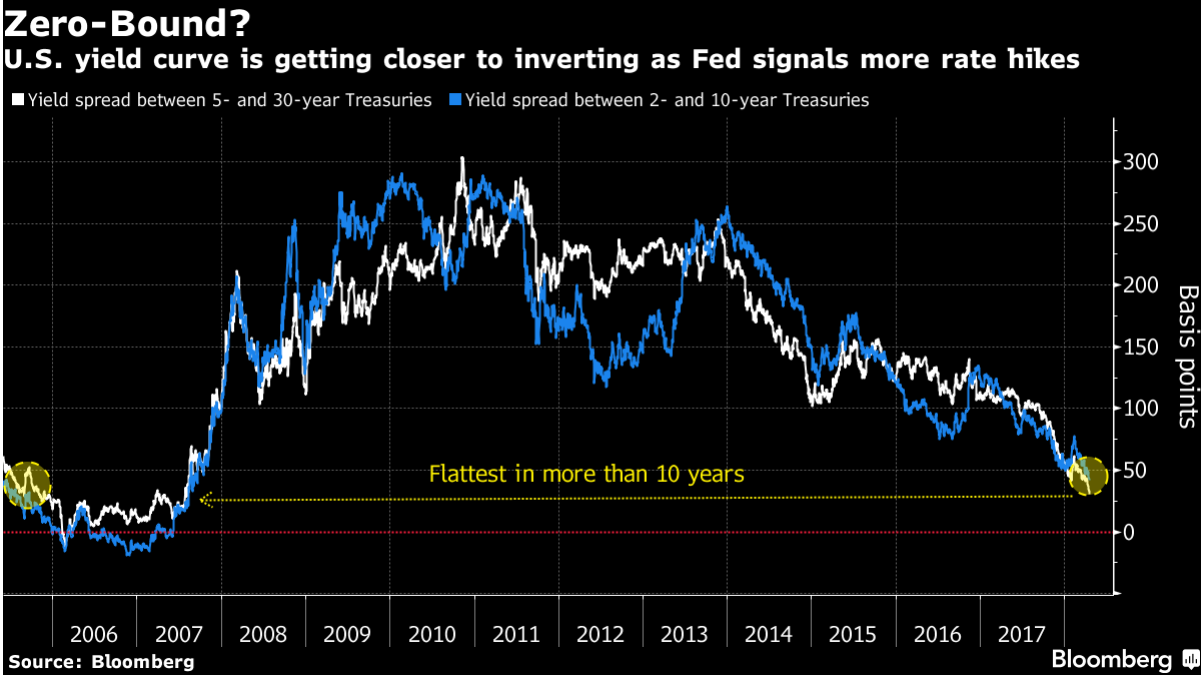
\includegraphics[width=1.3\textwidth]{images/flattening_yields.png}}
    \caption{Different yield spreads in April 2018, when the risk of yield curve inversion is real. We are reaching levels similar to the 2007 financial crisis. Not a good sign.}
    \label{fig:flattening_yields}
\end{figure}
\hspace*{-1cm}

“A potential curve inversion should be taken as seriously as always,” Citigroup analysts led by Jabaz Mathai wrote in an April 13 report. “The historical relationship between the curve and implied recession probabilities is highly non-linear: implied probabilities grow very fast when the curve moves into inverted territory.” Mathai argued that the Fed is wrong on the yield curve, again. He noted that in 2006, then-Chairman Ben S. Bernanke said he didn’t see inversion as portending an economic slowdown.

In the report, Mathai argued that the Fed is wrong on the yield curve, again. He noted that in 2006, then-Chairman Ben S. Bernanke said he didn't see inversion as portending an economic slowdown.

Last month, current Chairman Jerome Powell said “there are good questions about what a flat yield curve or inverted yield curve does to intermediation.” Though he added: “I don’t think that recession probabilities are particularly high right now.”
\chapter{MACROECONOMICS}
\begin{chapquote}{Roberto Bordin}
``La figa e' l'oppio dei popoli.''
\end{chapquote}

This is an additional chapter and can be useful to have a better understanding of what is going on in the world. The following sections are inspired by the online course available at \url{https://www.khanacademy.org/economics-finance-domain/macroeconomics}. It will be expanded in the future with more sections to cover more topics (Austrian economics for example).

\section{Circular flow of income and expenditures}
Imagine we have a country with only a firm and one family that owns the firm. The firm needs some factors of production building, land and labor to create products. This will produce some profit for the company. In this scenario, the family is buying from the firm, the firm is providing products to the family. On the other side, the family is providing the production factors to the firm and the firm is giving money to the family in form of wages, profit and rent for the other production factors. In this example, we have a family with the total expenditures, the firm with the total revenues, but also again the family with the total income. Expenditures and revenues are the same in this case, but all the revenues go to the family for paying the production factors and profit. Even if a bit artificial, this can be extended to the circular flow of money in a country with multiple firms and households. The gross domestic product (GDP) can be the total expenditures of the family, the total revenue of the firm or the total income of again the family, because they are all the same.

More formally, the GDP is the market value of all final products and services produced within a country in a given period. We do not count though illegal activity, or labor like a mother babysitting her own child. If the production of a good lasts longer than the period considered for computing the GDP, then the market value of the intermediate good (not finished yet) is considered. The following period will then consider the market value of the final good (assuming it is finished in this second period) minus the market value at the beginning of the period. Moreover, the goods taken into account are the ones produced within a country, regardless of the nationality of the producer. The gross national product (GNP) does instead take into account the nationality of the firm and not where the firm is based.

\subsection{How well GDP measures the well-being of society}
GDP is an indicator of a society’s standard of living, but it is only a rough indicator. 

GDP does not account for leisure time. The US GDP per capita is larger than the GDP per capita of Germany, but does this prove that the standard of living in the United States is higher? Not necessarily since it is also true that the average US worker works several hundred hours more per year more than the average German worker. The calculation of GDP does not take German workers extra weeks of vacation into account.

GDP includes what is spent on environmental protection, healthcare, and education, but it does not include actual levels of environmental cleanliness, health, and learning. GDP includes the cost of buying pollution-control equipment, but it does not address whether the air and water are actually cleaner or dirtier. GDP includes spending on medical care, but it does not address whether life expectancy or infant mortality have risen or fallen. Similarly, GDP counts spending on education, but it does not address directly how much of the population can read, write, or do basic mathematics.
GDP includes production that is exchanged in the market, but it does not cover production that is not exchanged in the market. 
GDP has nothing to say about the level of inequality in society. GDP per capita is only an average. When GDP per capita rises by 5\%, it could mean that GDP for everyone in the society has risen by 5\% or that the GDP of some groups has risen by more while the GDP of others has risen by less—or even declined.

GDP also has nothing in particular to say about the amount of variety available. If a family buys 100 loaves of bread in a year, GDP does not care whether they are all white bread or whether the family can choose from wheat, rye, pumpernickel, and many others—GDP just looks at whether the total amount spent on bread is the same.
Likewise, GDP has nothing much to say about which technology and products are available. The standard of living in, for example, 1950 or 1900 was not affected only by how much money people had—it was also affected by what they could buy. No matter how much money you had in 1950, you could not buy an iPhone or a personal computer.

In certain cases, it is not clear that a rise in GDP is even a good thing. If a city is wrecked by a hurricane and then experiences a surge of rebuilding construction activity, it would be peculiar to claim that the hurricane was therefore economically beneficial. If people are led by a rising fear of crime to pay for installation of bars and burglar alarms on all their windows, it is hard to believe that this increase in GDP has made them better off. In that same vein, some people would argue that sales of certain goods, like pornography or extremely violent movies, do not represent a gain to society’s standard of living.

The fact that GDP per capita does not fully capture the broader idea of standard of living has led to a concern that the increases in GDP over time are illusory. It is theoretically possible that while GDP is rising, the standard of living could be falling if human health, environmental cleanliness, and other factors that are not included in GDP are worsening. Fortunately, this fear appears to be overstated.
In some ways, the rise in GDP actually understates the actual rise in the standard of living. For example, the typical workweek for a US worker has fallen over the last century from about 60 hours per week to less than 40 hours per week. Life expectancy and health have risen dramatically, and so has the average level of education.
Since 1970, the air and water in the United States have generally been getting cleaner. New technologies have been developed for entertainment, travel, information, and health. A much wider variety of basic products like food and clothing is available today than several decades ago. GDP does not capture leisure, health, a cleaner environment, the possibilities created by new technology, or an increase in variety.
On the other side, rates of crime, levels of traffic congestion, and inequality of incomes are higher in the United States now than they were in the 1960s. Moreover, a substantial number of services that used to be provided, primarily by women, in the nonmarket economy are now part of the market economy that is counted by GDP. By ignoring these factors, GDP would tend to overstate the true rise in the standard of living.

A high level of GDP should not be the only goal of macroeconomic policy—or broader government policy. But, even though GDP does not measure the broader standard of living with any precision, it does measure production well, and it does indicate when a country is materially better or worse off in terms of jobs and incomes. In most countries, a significantly higher GDP per capita occurs hand in hand with other improvements in everyday life along many dimensions, like education, health, and environmental protection.

\subsection{Investment and consumption}
In everyday life, an investment is something that will give you a future gain like having a house, having a bond, studying, while consumption is when you use money to use up something and should make your life better in the short term.

In economy instead, investments are the creation of capital equipment, inventories for firms and construction of new houses while consumption is any spending on new final goods or services by households, except for new homes

For example, buying a car to go to work can be seen as an investment from the first perspective, but as a consumption from the second perspective.

\subsection{Expenditure view and components of GDP}
The GDP is made of the expenditures of the firms and of the households and of the government plus the exports minus the imports. To differentiate the expenditures between investment and consumption we can say that $Y = I + C + G + NX$, where $Y$ is the GDP and the other terms are the investments (both from firms and households), the consumption, the expenditures of the government and the net export. If an American firm is investing money on a foreign production factor, it means the investment value increases, but the net export decreases correspondingly and the total GPD does not change.

It's important to remember that a significant portion of government budgets are transfer payments—like unemployment benefits, veteran’s benefits, and Social Security payments to retirees—that are excluded from GDP because the government does not receive a new good or service in return or exchange. The only part of government spending counted in demand is government purchases of goods or services produced in the economy—for example, a new fighter jet purchased for the Air Force (federal government spending), construction of a new highway (state government spending), or building of a new school.

Since every market transaction must have both a buyer and a seller, GDP must be the same whether measured by what is demanded or by what is produced.
Everything that is purchased must be produced first. Instead of trying to think about every single product produced, let's break out five categories: durable goods, non-durable goods, services, structures, and change in inventories. 

You can see what percentage of the GDP each of these components contributes in the table and pie chart below.

\begin{figure}
\makebox[\textwidth][c]{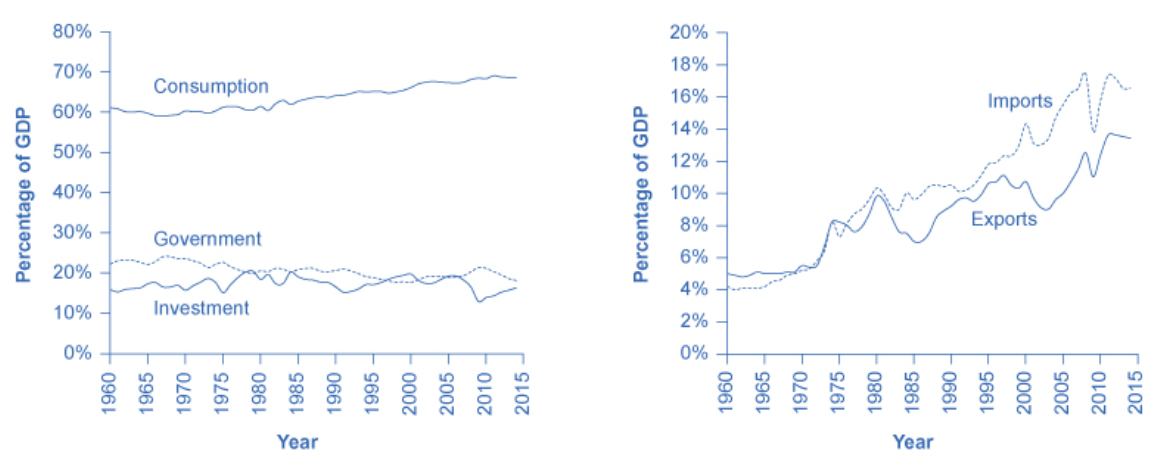
\includegraphics[width=1.1\textwidth]{images/USA_GDP.png}}
    \caption{GDP of the USA.}
    \label{fig:usa_gdp1}
\end{figure}

\begin{figure}
\makebox[\textwidth][c]{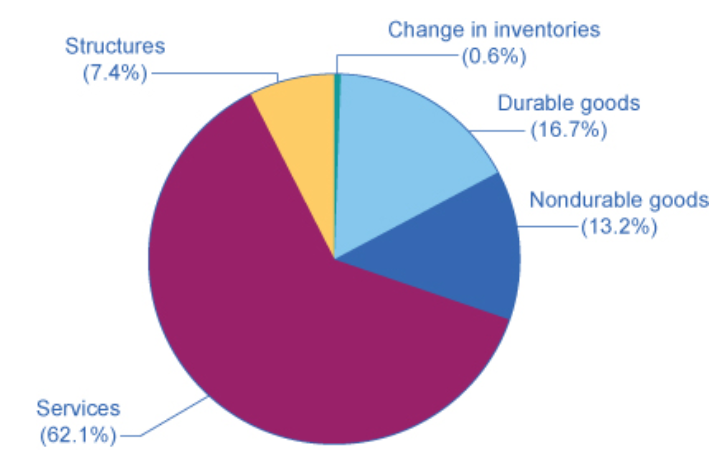
\includegraphics[width=1.1\textwidth]{images/USA_GDP_pie.png}}
    \caption{GDP of the USA.}
    \label{fig:usa_gdp_pie}
\end{figure}


The category of structures includes everything from homes to office buildings, shopping malls, and factories.
Inventories is a small category that refers to the goods that have been produced by one business but have not yet been sold to consumers and are still sitting in warehouses and on shelves.

The entire underground economy of services paid “under the table” and illegal sales should be counted—but is not—because it is impossible to track these sales. In a recent study by Friedrich Schneider of shadow economies, the underground economy in the United States was estimated to be 6.6\% of GDP, or close to \$2 trillion dollars in 2013 alone.

\subsection{Other ways to measure the economy}
Gross national product, or GNP, includes what is produced domestically and what is produced by domestic labor and business abroad in a year.
National income includes all income earned: wages, profits, rent, and profit income.
Net national product, or NNP, is GNP minus depreciation.
Depreciation is the process by which capital ages over time and therefore loses its value.

\subsection{Nominal and real GDP}
Let's say we have a country producing only oranges and at the end of year 1 we have a GDP equal to $Y_1 = N_1 p_1$, where $N_1$ is the amount of oranges produced in year 1 and $p_1$ is the price of one orange in year 1. At the end of year 2 we have instead $Y_2 = N_2 p_2$ and we can measure the growth of the country in this way: $G = Y_2 - Y_1$. Here, we are using the nominal GDP. If $G$ is positive, we might think that the economy is now larger than before, but did the country actually produced more goods than the previous year? Or in other terms, what is the GDP of year 2 in year 1's prices? This is the real GPD of year 2 and is equal to $Y_2' = N_2 p_1$.

\subsection{GDP deflator}
The GDP deflator is a measure of price inflation/deflation with respect to a specific base year; the GDP deflator of the base year itself is equal to 100.
\begin{equation}
GDP deflator = \dfrac{Nominal GDP}{Real GDP} 100
\end{equation}
The higher the GDP deflator, the lower the real GDP will be compared to the nominal GDP.

\subsection{Income and inequality}
\begin{figure}
\makebox[\textwidth][c]{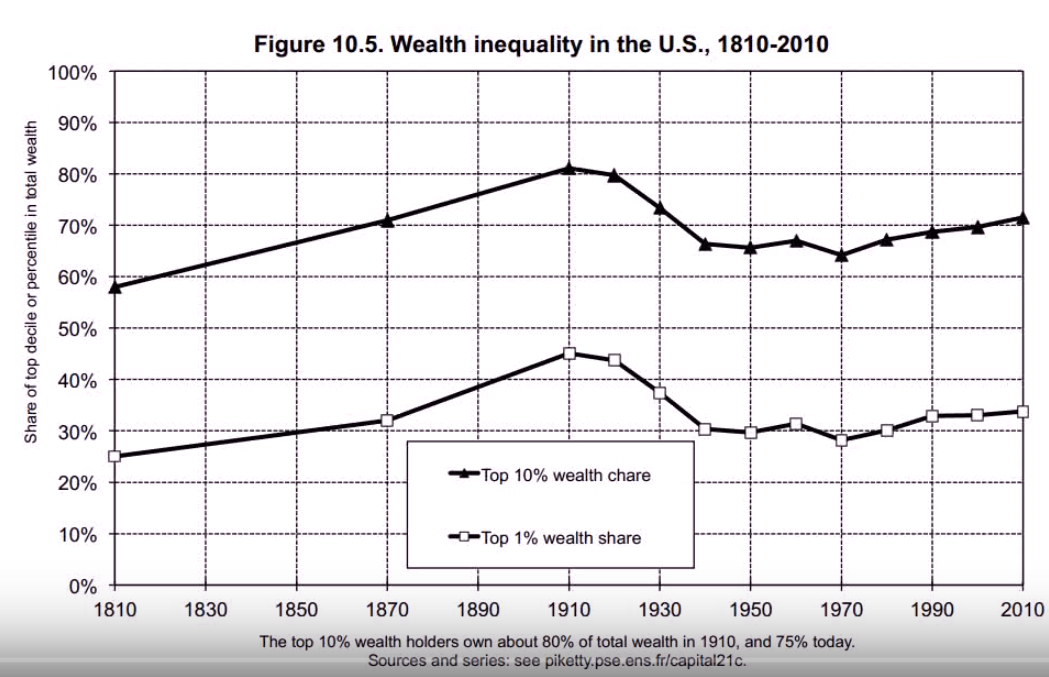
\includegraphics[width=1.1\textwidth]{images/piketty.png}}
    \caption{From Capital in the twenty-first century by Thomas Piketty.}
    \label{fig:piketty}
\end{figure}

Wealth is the total value of the assets owned by a person, which is different from its income. Thomas Piketty draws two possible theories of why we have income inequality. One is driven by labor where we have a mix of two possible reasons: the market recognizes the importance of top managers that are able to make big profits for the company, but also because these top managers are also self-regulating their income. The other theory is based on return on capital (ROC) and its relationship with the growth of the economy. If a person has a big amount of money inherited and she invest it, the ROC might be large enough to live without working. If the ROC is larger than the growth of the economy, the income inequality will grow. An example is the following. Alice gets \$100k in after-tax income, she spends \$80k and saves 20\% of her income, while Bob gets \$1M in after-tax income, spends \$400k and saves 60\%. Bob is getting richer because he's saving more, because it's easier to save money. As your income becomes smaller, it is more difficult to save. Because the saving rates generally goes up, more people will be in the situation of $r > g$, meaning that the ROC is greater than the growth of the economy. 

\begin{figure}
\makebox[\textwidth][c]{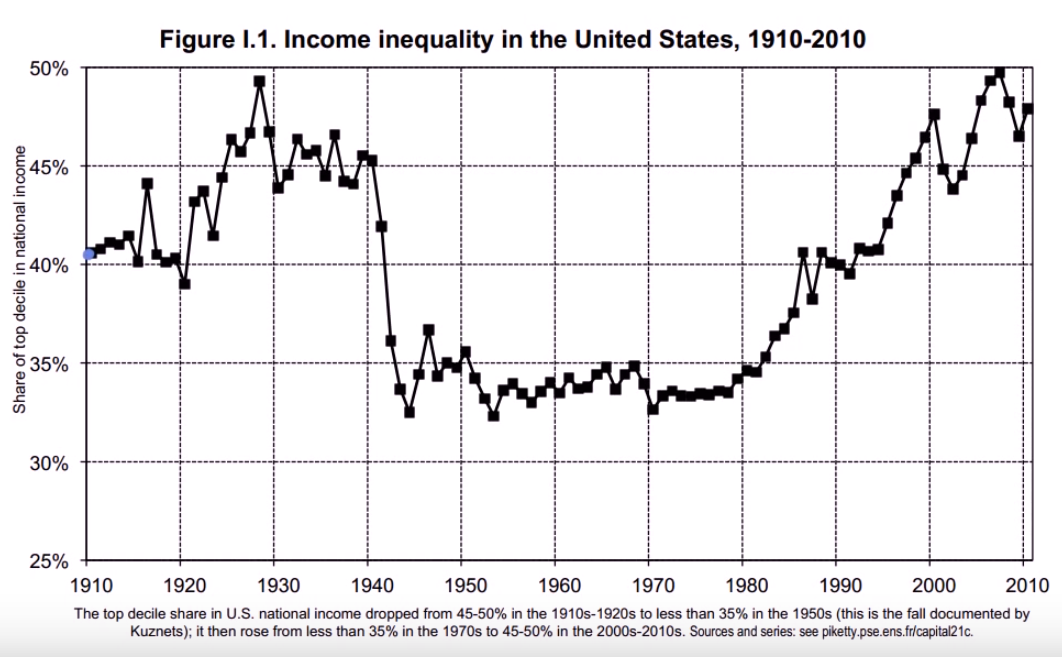
\includegraphics[width=1.1\textwidth]{images/income_ineq.png}}
    \caption{From Capital in the twenty-first century by Thomas Piketty.}
    \label{fig:income_ineq}
\end{figure}

A question to ask is: Is inequality always bad? There might be an example in which the answer is no.
Let's imagine a country in which the GDP is equal to 100 (whatever the currency) and the top 10\% of the people owns a third of the GPD. This means that the bottom 90\% of the population owns 67\% of the GPD, which means that each person in the bottom 90\% owns 0.741\% of the GPD, hence 0.741 (whatever the currency), and each person in the top 10\% holds 3.333\% of the GPD, hence 3.333 (whatever the currency). Now imagine a situation in which after one year, the GPD grew 10\%. This happens thanks to capital markets, which also bring more inequality. Let's also imagine that the top 10\% of the people holds now 35\% of the GPD which means two things: higher inequality and each of them has 3.5\% of the GDP, or 3.85 (because the GDP is now 110). But it also means that the bottom 90\% now has 65\% of the GDP, or 71.5 (whatever the currency), which means 0.794 for each person, larger than 0.741 of the previous year. So, in this example, we have growth, more inequality, but all the population got better. In general, if economic growth is enough, there will be a bigger pie for everyone. 

If you had to choose between a static economy and a personal income of X, or a growing economy and a personal income of X plus something, what would you choose? Remember that in the second case, someone will get a larger share of the growth than you, but still you will improve the quality of your life.

One force that was able to reduce inequality and led to more development in Asia after 1950 is education. In the gilded age (end of 19th century) there was no need of highly-skilled labor and capital had lot of importance in the production line. Now instead, especially with technology, more and more focus is put on educated labor (e.g., software and services).

Why does the value of private capital grow faster than national income? Imagine today you buy an asset (capital) with a value $V$ and it will give you a ROC of $r$, so the income is $rV$. In few months, for some reason, the same asset will give an income of $2rV$, but because there is a lot of people demanding this asset now, its value is $2V$, hence its ROC is still $r$. This means that people are still willing to have that asset with the same ROC, but the value of the capital and the income it generates has increased. But it could also happen the opposite, where the income decreases, then the value decreases and the ROC remains the same. Another possible scenario is when there is more money and less profitable businesses. In this case, people will be willing to have a lower ROC, so if the income is still $rV$, but $r$ is lower, than $V$ must increase.

Today:
\begin{itemize}
    \item V = 100
    \item I = 10
    \item r = 10\%
\end{itemize}
Tomorrow with more profitable businesses (in terms of income), but more people investing:
\begin{itemize}
    \item V = 200
    \item I = 20
    \item r = 10\%
\end{itemize}
Tomorrow with less profitable businesses (in terms of income), and less people investing:
\begin{itemize}
    \item V = 50
    \item I = 5
    \item r = 10\%
\end{itemize}
Tomorrow with less profitable businesses (in terms of ROC), and more people investing:
\begin{itemize}
    \item V = 200
    \item I = 10
    \item r = 5\%
\end{itemize}
Tomorrow with less profitable businesses (in terms of ROC), and less people investing:
\begin{itemize}
    \item V = 50
    \item I = 2.5
    \item r = 5\%
\end{itemize}

\subsection{Bond prices and interest rates}
If in this moment the interest rates increase, the prices of the bonds available in the market few seconds ago will decrease.

Let's illustrate this with a \$100,000 bond having a stated interest rate of 9\% and having a remaining life of 5 years. This bond will pay \$4,500 at the end of each of the 10 remaining semiannual periods plus \$100,000 at the end of the bond's life. If an investor's goal is to earn 9\%, the investor will pay \$100,000 for the bond. However, if the market interest rates increase to 10\% the investor will now be able to earn \$5,000 semiannually on a \$100,000 investment. Obviously, the 9\% bond paying only \$4,500 semiannually will no longer be salable for \$100,000.

For an investor to buy the 9\% bond in a 10\% market, the bond's price will have to drop to an amount that will yield a 10\% return over the bond's remaining life. Using our example, the investor will earn 10\% only if the 9\% bond can be purchased for approximately \$96,000. The cash return of \$4,500 every six months for five years on the \$96,000 investment plus the gain of \$4,000 (\$100,000 in 5 years versus the investment of \$96,000) will result in the required return of 10\%.


\section{Inflation: measuring the cost of living}

\subsection{Unintended redistributions of purchasing power and inflation}
Inflation can cause redistributions of purchasing power that hurt some and help others. People who are hurt by inflation include those who are holding a lot of cash, whether it is in a safe deposit box or in a cardboard box under the bed. When inflation happens, the buying power of cash is diminished. But cash is only an example of a more general problem: anyone who has financial assets invested in a way that the nominal return does not keep up with inflation will tend to suffer from inflation. For example, if a person has money in a bank account that pays 4\% interest, but inflation rises to 5\%, then the real rate of return for the money invested in that bank account is negative 1\%.

The US income tax is charged on the nominal interest received in dollar terms, without an adjustment for inflation. So, a person who invests \$10,000 and receives a 5\% nominal rate of interest is taxed on the \$500 received—no matter whether the inflation rate is 0\%, 5\%, or 10\%. If inflation is 0\%, then the real interest rate is 5\% and all \$500 is a gain in buying power. But if inflation is 5\%, then the real interest rate is zero and the person had no real gain—but they owe income tax on the nominal gain anyway. If inflation is 10\%, then the real interest rate is negative 5\%, and the person is actually falling behind in buying power. But, they would still owe taxes on the \$500 in nominal gains.

Inflation can cause unintended redistributions for wage earners, too. Wages do typically creep up with inflation over time—eventually. However, increases in wages may lag behind inflation for a year or two since wage adjustments are often somewhat sticky and occur only once or twice a year. Also, the extent to which wages keep up with inflation creates insecurity for workers and may involve painful, prolonged conflicts between employers and employees. 
Ordinary people can sometimes benefit from the unintended redistributions of inflation as well. Consider someone who borrows \$10,000 to buy a car at a fixed interest rate of 9\%. If inflation is 3\% at the time the loan is made, then the loan must be repaid at a real interest rate of 6\%. But if inflation rises to 9\%, then the real interest rate on the loan is zero. In this case, the borrower’s benefit from inflation is the lender’s loss. A borrower paying a fixed interest rate who benefits from inflation is just the flip side of an investor receiving a fixed interest rate who suffers from inflation. The lesson is that when interest rates are fixed, rises in the rate of inflation tend to penalize suppliers of financial capital, who end up being repaid in dollars that are worth less because of inflation. At the same time, demanders of financial capital end up better off because they can repay their loans in dollars that are worth less than originally expected.

When inflation causes a retiree who built up a pension or invested at a fixed interest rate to suffer while someone who borrowed at a fixed interest rate benefits from inflation, it is hard to believe that this outcome was deserved in any way. 

A firm can make money from inflation—for example, by paying bills and wages as late as possible so that it can pay in inflated dollars, while collecting revenues as soon as possible. A firm can also suffer losses from inflation, as in the case of a retail business that gets stuck holding too much cash only to see the value of that cash eroded by inflation. But when a business spends its time focusing on how to profit by inflation, or at least how to avoid suffering from it, an inevitable trade-off strikes: less time is spent on improving products and services or on figuring out how to make existing products and services more cheaply. An economy with high inflation rewards businesses that have found clever ways of profiting from inflation, which are not necessarily the businesses that excel at productivity, innovation, or quality of service.

Traditionally, government bonds have paid a fixed rate of interest. This policy gave a government that had borrowed an incentive to encourage inflation because it could then repay its past borrowing in inflated dollars at a lower real interest rate. But indexed bonds promise to pay a certain real rate of interest above whatever inflation rate occurs. In the case of a retiree trying to plan for the long term and worried about the risk of inflation, for example, indexed bonds that guarantee a rate of return higher than inflation—no matter the level of inflation—can be a very comforting investment.

\subsection{Phillips curve}

Irving Fisher, and later William Phillips, showed that there is an inverse relationship between unemployment and inflation: High inflation means higher prices due to higher demand, due to higher wages, due to more leverage for workers, due to lower unemployment. Two exceptions must be considered. The first happened in 1970, when the oil supply suddenly decreased and drove the prices up, but it was not due to higher wages, so there chain presented above was broken. The second happened with the technological revolution where more demand did not cause lower unemployment because of higher production and production efficiency.

\section{Aggregate demand and aggregate supply}
\subsection{Aggregate demand}
Aggregate demand is the amount of total spending on domestic goods and services in an economy.

In microeconomics, production and prices have a negative correlation: all else being equal, more production means lower price. Some economists claim that this is true also in macroeconomics and the aggregate demand curve is similar to the downward-sloping demand curve. There are three theories supporting this. If one day, prices decrease within a country, people will have more buying power, so they could buy more or save more. In the first case, they directly stimulate more production, while in the second case they put more money in the banks, which will be able to lower interest rates and make more investments and then the general production of the country increases. The third case is still based on the fact that interest rates are lower and investors would convert money into another currency with higher interest rates, making the own country's currency weaker, stimulating export, hence more production (GDP).

If the GPD is the sum of consumption, investments, government spending and net export, then any increment in one of these factors will move the curve right.

\subsection{Aggregate supply}
Aggregate supply is the total quantity of output firms will produce and sell—in other words, the real GDP. 

In the long term, which means a period in which fixed contracts expire, real GDP does not change with the prices. It increases or decreases though thanks to other factors: increase in population, higher employment, technological 
improvement, wars, discovery of new resources. In the long run, the price doesn't matter because any increases or decreases in price will be cancelled out by decreases or increases in costs (wages, input costs, etc.). If prices double, so do wages, so people have no additional spending power. Firms will produce the same and households will buy the same.

Over time, productivity grows so that the same quantity of labor can produce more output. Historically, the real growth in GDP per capita in an advanced economy like the United States has averaged about 2\% to 3\% per year, but productivity growth has been faster during certain extended periods.

In the short term instead, we have an upward-sloping aggregate supply curve, because when the price level for outputs increases while the price level of inputs remains fixed, the opportunity for additional profits encourages more production.

Demand curves for individual goods or services slope down primarily because of the existence of substitute goods, not the wealth effects, interest rate, and foreign price effects associated with aggregate demand curves.

\subsection{Demand-pull and cost-push inflation}
In the '60 the US president Johnson kept spending and investing at an excessive level. This put more money into people's pockets and the real GDP increased, shifting the aggregate demand curve to the right. The equilibrium between aggregate demand and aggregate supply on the short was at a higher level of prices and of real GDP (beyond the natural level). On the long term though, the aggregate demand must meet the aggregate supply on the long run, so the prices are higher if aggregate demand does not go back to its previous level.

In the 1973 we had the oil embargo in the US that led to higher prices in general, without any increment in the real GDP. This led to shift the short term aggregate supply curve to the left, because it was more expensive to produce goods. This is stagflation.

\subsection{Monetary and fiscal policy}
How is the demand and supply for the money market? On the x-axis we have the money supply (how much money are available to be borrowed/lent), on the y-axis we have the price of borrowing, namely interest rates. The demand curve is decreasing with supply because the cheaper the cost of money, the higher the number of people willing to borrow for their projects. Very few projects have high returns and many projects have low returns. The aggregate supply instead is increasing: the higher the interest rate, the better for the supplier (lender), the higher the number of lenders. 

When the central bank lends money, it is shifting the supply curve to the right, making it easier for people to borrow money and start businesses and to spend money, leading to an increase of aggregate demand. This is known as monetary policy.

Fiscal policy is instead used by the government to stimulate or slow down demand leveraging on taxes and debt. This policy has usually a more direct effect.

\subsection{Keynesian economics}
The classical model for aggregate demand and aggregate supply in the long run is a vertical line for LRAS and a downward-sloping AD. The only way to increase the output of the country is by making it more productive through investments in technology or increase population for example, to shift the LRAS to the left. Just flooding the economy with newly printed money will increase the demand, but in the long run aggregate supply will not change, only prices and inflation will.

One reasoning that makes sense is the following: If the economy is working at full capacity, people will be very busy to work, they would make good money and don't need to work extra time to survive. If they are asked to do extra work, they would ask for a pay raise and prices would go up. On the other hand, if unemployment is high, people will not ask for higher salaries and in the short run, they will be willing to get the same salary regardless of working time. If a factory is running at \%30 capacity and people wants to buy more from me, I'm not going to raise prices because I still need to attract clients. In other words, at low capacity and in the short run prices are sticky compared to production.

In the '30, during the Great Depression factories and people were available to work, but aggregate demand decreased significantly and quickly. The economy was producing below its capacity. At this point, Keynes believed that the SRAS is a horizontal line. In this case the only way to increase GPD is to increase the aggregate demand, through monetary policy or fiscal policy.

In conclusion, the most appropriate model is a mix of classical and Keynesian economics. At low real GDP levels, prices do not change with production and the government should increase the aggregate demand, while at high real GDP levels production does not change with prices and if the government wants to further increase production, it should increase population of production efficiency.

The risk associated to Keynesian politics is that once the government intervenes through fiscal policy (taxes or spending), it becomes difficult and unpopular to stop these stimuli and this might lead to a overheated economy and a growing inflation without a corresponding increase in real GDP because everything is spent on consumption and nothing is saved for technological improvements\footnote{I think the key part here is how the government is using the extra money obtained through monetary or fiscal policy. With Keynesian politics, it should use it to increase aggregate demand, ignoring investments to increase the aggregate supply. What if instead some part if it is used also to increase the aggregate supply?}.

\begin{figure}
\makebox[\textwidth][c]{
    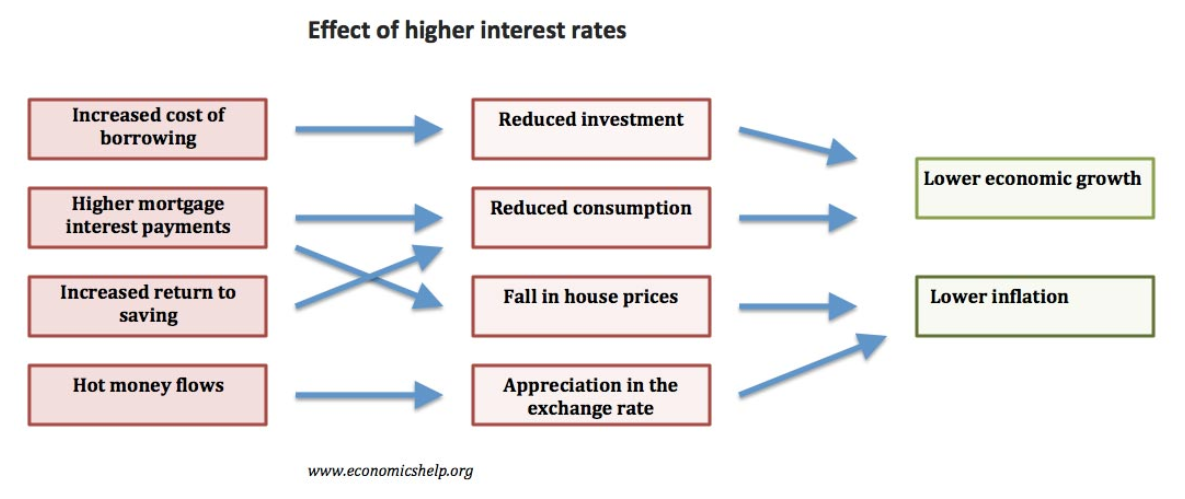
\includegraphics[width=1.1\textwidth]{images/high_rates.png}
}
    \caption{Why should a central bank make borrowing more difficult?}
    \label{fig:high_rates}
\end{figure}

The Central Bank usually increase interest rates when inflation is predicted to rise above their inflation target. They increase the cost of borrowing, reduce disposable income and therefore limit the growth in consumer spending. Higher interest rates tend to reduce the rate of economic growth and inflationary pressures. Higher interest rates make it more attractive to save in a deposit account because of the interest gained and increase the value of a currency because more people will save money in banks of that country. A government will face higher borrowing costs and might raise taxes to deal with this problem. A person who likes to save money in banks wants low inflation and high interest rates. A borrower (fixed interest rate) prefers high inflation and low interest rates.

\section{Income and expenditure: Keynesian cross and IS-LM model}

\subsection{MPC}
Imagine I find on the street a sum of money $S$ and I take it. What I do next is to spend part of it, let's say, $r = 60\%$. I decide to spend $S' = rS$ to buy oranges and lemons from the market on the street. The merchant is pretty happy because I usually don't buy products from him, but now he has more money than yesterday. He decides to spend a fraction of the money he just received from me by buying a new pair of shoes for exactly $S'' = rS'$, a fraction of which will be spent again and again. If we assume we can find an average value for $r$ in the whole economy, we will get the Marginal Propensity to Consume.

\subsection{Consumption function}
People need to consume food, electricity and other stuff to survive, so even if they have no income, they'll still consume a basic amount of products and services. Let's call it $c_0$. In addition to that, they will also spend a fraction of their disposable income, which is the income minus taxes. This fraction is the MPC from the previous section. Recall that the aggregate income is equivalent to the GDP. We can then write the total consumption as follows:

\begin{equation}
C = c_0 + MPC(Y-T) = MPC \cdot Y + (c_0 - MPC)T.
\end{equation}

This model is obviously simplifying the reality as, instead of a linear relationship between disposable income and consumption, we can have a model which takes into account the fact that it is easier to save with higher disposable income.

\subsection{Keynesian cross}
What are the aggregate planned expenditures of a country? They are the sum of: consumption, planned investments, government spending and net export. If we make one big simplification and assume that, except for consumption, these terms do no depend on the GDP, then the planned expenditures are modeled as linear in Y (consumption is assumed linear with the GPD). So, if we were to plot how the planned expenditures change with the GPD, we would get a linear function with positive intercept and positive slope. Furthermore, we know from history and economics, that when an economy is at equilibrium, the aggregate planned expenditures equal the aggregate output, the GDP, which means it is represented by a bisector. This bisector will meet the planned expenditures creating the Keynesian cross indicating where the economy is at equilibrium. If the GPD is higher than this point, inventories will build up and the planned investments were lower than the actual investments. Of course every company will adapt its production to the current demand, so any excess or lack of goods will decrease. 

If inventories are building up, is because expenditures are too low. In line with Keynesian thinking, to bring the economy to an equilibrium, but without decreasing the GDP, the government can step in and increase its involvement in the expenditures. This will shift the crossing point to the right (higher GDP) more than the upward shift (higher expenditures). This is due to the multiplier which turns out to be $m = \dfrac{1}{1-MPC} > 1$. This means that any increment in consumption through taxes or government spending, will lead to a greater increment in the GDP.

The Keynesian model in general says that you can drive growth through fiscal policy, be it through taxes or government spending (both in increasing and decreasing terms).

\subsection{IS-LM model}

If interest rates are $r$, only the projects with an expected return greater than $r$ will be financed, hence higher interest rates means less planned investments and lower expenditures as seen in the previous section and the Keynesian cross moves and, at equilibrium, lower GDP. On the other hand, lower interest rates means higher GDP.
We can also manipulate the formula for GDP in the following way:

\begin{equation}
    Y = C(Y) + I + G + NX \\
    Y - C(Y) - G = I + NX.
\end{equation}

If we assume the net export is zero, we can see that investments are equal to a term which represents the savings of the country.
IS in the IS-LM model stands for Investments-Savings and we just saw they are the same thing.

LM instead stands for Liquidity preferences and Money supply. Next, we need to define what is real money: The ratio between $M0$ and the consumer price index (CPI), so it's money adjusted for inflation. Let's assume this number is constant, which is a big assumption. Now, the more economic activity there is, the higher the demand for this money so when the economy is close to its full capacity and high GDP, people is willing to pay higher prices for money, while when GDP is low people are not willing to pay much for it. This is the liquidity preference. We can model this relationship with a linear function with positive slope, which will meet the IS model at the equilibrium. Finally, if the central bank decides to print money, the demand will be lower and the interest rates would decrease, shifting the crossing point to the left with higher GDP.

How does government spending affect this model? We know that a higher $G$ in the planned expenditures will lead to higher GDP. On the IS-LM model this means that the IS function will shift right, which in turn leads to a shift of the crossing point with the LM model (up and right). The LM model itself does not change in the short term.

\section{Foreign exchange and trade}
\subsection{Speculative attack on a currency}

When a central bank wants to keep its currency A weak compared to a foreign currency B (to stimulate export for example), it prints more of its money and use it to buy B. Let's assume the exchange rate is pegged to $25A = 1B$ or $r = 0.04A/B$. If more people want to convert B into A, maybe because they want to invest in this country, the central bank of A will print more money and buy B to keep $r$ stable.

In 1996, the currency of Thailand, THB (Thai Baht), had an exchange rate of $25THB = 1USD$, and short-term interest rates were higher in Thailand. Let's imagine the followig scenario now. I borrow \$1M with an interest rate of 8\% (2 year loan), I convert my dollars into THB and I lend them to some business in Thailand where a 2-year loan has an interest rate of 12\%. After 2 years, if my investment was good, I get my THB plus interest back and I convert them into USD and I pay back my 2-year loan in USD. With these numbers, I would make a profit of \$40K, just by playing on interest rates and the exchange rate that I assume is fixed by the Thai central bank. 
Where is the risk here? The risk is that the exchange rate may change. The Thai central bank can only print its currency and so keep THB weak compared to USD, but when many people want to convert THB into USD, the Thai central bank has just a limited reserve of USD (depending on how many US dollars it bought in the past). In this scenario, there is higher demand of USD and it becomes more expensive to convert THB to USD, which means the exchange rate can be now something like $45THB = 1USD$. With this new rate, the previous investment would bring you big loss, because the THB devaluated and when converted to USD it would worth much less. What happened in Thailand was that many people saw this initial opportunity of arbitrage, financed many activities in Thailand, a bubble started to appear, people got scared and started to convert THB back to USD. 

A speculative attack in this case means that people believe the Thailand central bank has not enough USD to keep the exchange rate fixed and THB will devaluate. What a speculator would do here is the opposite of what has been described above: borrow a sum in THB, convert it into USD, lend the sum, get it back after some time, convert USD into THB which will give more money because the THB has devalued, pay back the loan in THB, and make money because of the THB devaluation. The more people do this, the higher the devvaluation, the higher the profit for speculators.
% \chapter{MICROECONOMICS - 14.01}

\section{Market inefficiency}
If prices for a good increase, we are not immediately able to tell if it was due to a shift in the demand or in supply. 

In the labor market, the firms are the demand, the workers are the suppliers. The supply curve with hours worked per year on the x-axis and wage on the y-axis is an upward-sloping, because the higher the wage, the more you're willing to work. The demand is instead downward-sloping: the higher the labor cost, the lower the number of people hired (machines would maybe replace them).

Right-wing people would support markets and let them free to evolve as they always tend to equilibrium. Left-wing people is instead prone to government intervention. 

An example is the introduction of minimum wage. If this minimum wage is above the current equilibrium, firms will be willing to hire less workforce at the minimum wage and workers will be willing to work more for the minimum wage. This gap is unemployment. If the minimum wage is below the equilibrium it would be ignored.

Another example is the following. Imagine we have problems in oil production and the supply curve moves up, but the government decided to put a cap on the price of oil to bring it back to the previous price. This would lower the price but would also create an excess in demand. At this lower price, oil producers will be willing to produce less, while consumers to buy more.

Efficiency in markets is when every trade which makes both parties better off is made, without interference from other parties. When this does not happen, markets become inefficient and losses occur. In the two examples above we have inefficiency in that unemployed people might be willing to work for a wage lower than the minimum and firms might be willing to hire people for a lower wage, but this cannot happen. Same point for the oil price cap: People that do not get enough oil are willing to pay more to have it, instead of waiting in line and waste time, and oil producers are willing to provide more oil for a higher price, but this cannot happen. Allocation inefficiency occur. The benefit though is that with these measures, there is more equity in the sense of fairness: everybody can get oil regardless of how rich they are, everybody can compete to have a minimum wage, and nobody is underpaid (despite some are not paid at all).

One solution to the problem of oil shortages (or also water shortages) would be to create secondary markets where people gets a minimum amount of the resource, decided by the government, and they can trade it depending on their needs.

The efficiency in the market would also mean that Americans and Europeans should ship their garbage to Africa and pay for it because we have money and garbage, they have land to store garbage and no money. Both parties would be better of.

\section{Elasticity in demand}

When a product has a perfect substitute (imagine two very similar kinds of biscuits for example), then the price of the product is perfectly elastic, because one can immediately change it with its substitute. In the other extreme, a product with no substitute (imagine a specific medicine) is perfectly inelastic in price to shifts in supply. One would always buy the product, regardless of its price. The percentage change in quantity over the percentage change in price is the elasticity of a product. The two extreme scenarios presented above correspond to negative infinite elasticity and zero elasticity.

\begin{equation}
    \epsilon = \dfrac{\Delta Q/ Q_i}{\Delta P/ P_i}
\end{equation}
Where $P_i$ is the initial price before the shift.
The change in revenue with respect to the change in price is:
\begin{equation}
    \Delta R / \Delta P = Q (1 + \epsilon).
\end{equation}
Hence, when elasticity is greater than -1, it makes sense to increase prices. To determine elasticity one need empirical economics and not theoretical economics. In particular, we need to know the multiplier of the demand curve (not the multiplier of the supply curve otherwise we confuse causation with correlation).

What if there is a new tax on a specific product and this product is completely elastic? The producer will try first to increase the price, to cover the taxes, so the supply curve shifts up, but the equilibrium will be at the point where the price is the same as before and lower production. When the government wants to raise money through taxes, it should do so taxing inelastic products. Liberals might want to raise taxes on yachts, but they are very elastic, while cigarettes are not. When the politicians or journalists say the government will raise a certain amount of money by taxing a specific good, they are just reporting the best estimates. Also, elasticity cannot be constant with big supply or demand changes.


\section{Stock options to managers}

if a manager is given stocks of his company, he will take decisions more wisely and avoid risky moves. If he gets stock options instead he will take risky decisions because he will not get the downsize of a bet. If the company loses value, he is covered by the (call) option. Investigation done by the WSJ revealed that many managers were given backdated stock options, meaning that they were artificially issued the day before the company's value increased and the manager was given free money in an apparently-legal way. This is of course fraud, but the managers don't care because if they get caught, they'll pay a fine for a third of what they made.

% monopsony is the power of a company over its labour. People prefer to work with the company at a lower wage despite the fact that there are other companies paying more. This is because the worker can't leave the city of the company or does not have other skills for change company. In this case a well-set minimum wage can reduce unemployment, just like a monopoly with a regulated price can improve welfare. How can this be possible? Maybe companies can afford to pay more and still be able to operate. Higher wages means more consumption and more demand and more supply and higher wages.

When we say we want to redistribute money from richer to poorer people, we can not simply take money from richer people and put it in a bucket and give this bucket to poor people, because there is two sources of leakage. First, we increase taxes on rich people and they will start to work less hard and production decreases and the pie shrinks. Second, almost poor people will start quit their jobs to qualify as poor and this also shrinks the pie. Social waste, deadweight loss arises from this redistribution system. Is it worth it? You need to solve the social welfare function, which we have to choose. Equity-efficiency trade off.
In the US, for every dollar they try to put in the bucket, roughly 40 cents leak out.
To reduce this leakage, targeted redistribution of income was implemented: poor disable people and poor single-parent family receive money.

Income is consumption plus savings. In the US, income is taxed more than in Europe, where consumption is taxed more instead. In Europe, hence, savings are not as taxed as in the US and they are promoted. But consumption taxation is very regressive, it hits the poor more than the rich. Governments in Europe though make sure to take care of poor people.

The United States federal earned income tax credit or earned income credit (EITC or EIC) is a refundable tax credit for low- to moderate-income working individuals and couples, particularly those with children. The amount of EITC benefit depends on a recipient's income and number of children. It works as a patch to the bucket.

In the US, \$80B a year are associated to costs for smoking. Smoking, obesity, alcohol, gasoline.

to solve the asymmetric information in insurance the government can do two things: subsidize or mandate. The first, the government pays the insurance for everyone, but has to raise taxes and everyone is affected. The second, the government by law says everyone must buy an insurance. In this case people not in need of an insurance will be upset. In the first case we have inefficiency in raising taxes and taxpayers will be upset. There is no correct answer in this market failure.
\chapter{SCANDALS}
\begin{chapquote}{Jeb Hensarling}
``How can we have capitalism on the way up and socialism on the way down? If we lose our ability to fail will we not in turn lose our ability to succeed?''
\end{chapquote}

What follows is not part of the Khan Academy's course, rather an analysis of some of the scandals related to finance in recent times. This will help myself and the reader to better understand when and how finance can be harmful for society.

\section{Cartel Bank}
% anabel hernandez - Mexican journalist
% victor avila - special agent
% sinaloa region cartel
% ken del valle - criminal defense attorney
% patrik radden keefe - the new yorker
% matt taibbi - rolling stone
% william ihlenfeld - us attorney
% brett wolf - anti-money laundering correspondent thomson reuters
% Loretta Lynch, US attorney, condemned HSBC to pay a fine 
Imagine a guy in Mexico with a regular job. He has to work for more than six months to get \$3000, but he also has the choice to cross the US border driving a car with 300 pounds of marijuana, stop at a shopping mall for few hours, get back to the car with no more drug in it and come back home. He would make the same amount of money in one afternoon. And this is not the difficult part. The drug will be sold on the street and lots of cash will be collected. The difficult part is then to put these US dollars into the financial system. Or maybe it's not so difficult. 

"Plata o plomo", silver or lead, bribe or death. These are the famous words usually told to a banker to convince him to launder the money. In Mexico, there was a bank called Banco Bital, with a strong business in regions related to drugs. Banco Bital was bought by HSBC in 2002 and it said that Bital was not a risky bank.

HSBC Holdings plc is instead a British multinational banking and financial services holding company. It is the largest bank by total assets in Europe with total assets of US\$2.374 trillion (as of December 2016). HSBC stands for Hongkong Shanghai Banking Corporation.

Zehnli Ye Gon, a Mexican also known as el Chino, was running Unimed, a pharmaceutical business and it was used to bring meth into the US. In his mansion, guns and stacks of cash (205 million USD) were found. He was a customer of HSBC Mexico. HSBC London ordered to close his bank account in 2004, but it was not closed.

Barton Joseph Adams, a doctor in West Virginia, was running Interventional Pain Management. He prescribed opioid to his patients, committing fraud with Medicare and West Virginia Medicaid. He underreported his income coming from this scheme and laundered money. The transactions were with HSBC. Adams was just the tip of the iceberg. Many of the other transactions found were related to terror financing, Russian criminals and more.

In light of this scandal HSBC was forced to assume people and clear these transactions. Everett Stern was one of those, but he was not a criminal, nor a stupid. He was asked to go through the system and close the alarms related to these transactions. He discovered that HSBC allowed transactions from criminal organizations, such as Tajco, a financial supporter of Hizballah, one of the most dangerous terrorist groups in the world. The OFAC sanctions list contains details about these entities and Tajco is one of them. 

Stuart Levey, Chief Legal Officer of HSBC and treasury official of the United States, and Irene Dorner  CEO of HSBC Bank, admitted the mistakes many times, but did not solve the problems. The discussion between Senator Carl Levin and the HSBC bosses looks very similar to the one Mark Zuckerberg had with the senators in light of the Cambridge Analytica scandal.

William Ihlenfeld, an attorney in West Virginia was asked to step down when he reported the problems with Doctor Adams. He was said to stand down from looking at HSBC.
HSBC paid a fine of \$1.9 million, five week's profit and a deferred prosecution agreement (DPA) was made. A deferred rosecution agreement is very similar to a non-prosecution agreement (NPA). It is a voluntary alternative to adjudication in which a prosecutor agrees to grant amnesty in exchange for the defendant agreeing to fulfill certain requirements. In this case, these requirements were to partially defer bonus compensation for its most senior executives. Wow! A journalist during the conference raised the point that the fine HSBC paid was small compared to what they did. The answer from Lanny A. Breuer, an American lawyer was: "Our goal here is not to bring HSBC down, it's not to cause a systemic effect on the economy, it's not for people to lose thousands of jobs", and the journalist "Don't they [the senior executives probably] deserve that?". No individual was fined, no one went to jail.

Eric Holder, Attorney General of the United States from 2009 to 2015, was asked not to indict HSBC Bank and he agreed. It happened when the US was coming out of the 2007 financial crisis and another hit to a bank would have raised alarms again.

Elizabeth Warren: "If you're caught with an ounce of cocaine, you'll likely go to jail. If it happens repeatedly, you may go to jail for the rest of your life. But evidently, if you launder nearly a billion of dollars for drug cartels and violate our international sanctions, your company pays a fine and you go home and sleep in your own bed at night. Every single individual associated with this. I think it's fundamentally wrong. That is not equal justice under law".

In 2012, the same year HSBC avoided prosecution, over 90,000 people were sentenced to federal prison for drug offenses in the USA. Since 2002, over 100,000 people have been killed in Mexico as a result of drug cartel violence. From 2002 to 2014, heroin-related overdose deaths in the USA more than quadrupled.

From the official document \citep{HSBC}:

"From 2006 to 2010, HSBC Bank USA violated the BSA [Bank Secrecy Act of 1970] and its implementing regulations. Specifically, HSBC Bank USA ignored the money laundering risks associated with doing business with certain Mexican customers and failed to implement a BSA/AML [Anti Money Laundering] program that was adequate to monitor suspicious transactions from Mexico.

As a result of these concurrent AML failures, at least \$881 million in drug trafficking proceeds, including proceeds of drug trafficking by the Sinaloa Cartel in Mexico and the Norte del Valle Cartel in Colombia, were laundered through HSBC Bank USA without being detected. HSBC Group was aware of the significant AML compliance problems at HSBC Mexico, yet did not inform HSBC Bank USA of these problems and their potential impact on HSBC Bank USA’s AML program.

There were at least four significant failures in HSBC Bank USA’s AML program that allowed the laundering of drug trafficking proceeds through HSBC Bank USA:
a. Failure to obtain or maintain due diligence or KYC [Know Your Customer] information on HSBC Group Affiliates, including HSBC Mexico; 
b. Failure to adequately monitor over \$200 trillion in wire transfers between 2006 and 2009 from customers located in countries that HSBC Bank USA classified as “standard” or “medium” risk, including over \$670 billion in wire transfers from HSBC Mexico; 
c. Failure to adequately monitor billions of dollars in purchases of physical U.S. dollars ("banknotes") between July 2006 and July 2009 from HSBC Group Affiliates, including over \$9.4 billion from HSBC Mexico; and 
d. Failure to provide adequate staffing and other resources to maintain an effective AML program."

On December 11, 2017, the US Department of Justice announced its plans to dismiss all criminal charges against HSBC

The whole story at \url{https://www.netflix.com/title/80118100}

% \section{Hard NOx}

% % alex gibney - director
% % sally yates - deputy attorney general
% % jack eving - reporter
% % walter groth - ex executive of volkswagen
% % Ferdinand piech - vw and audi executive
% from year 2009 to 2015, 500 000 diesel vehicles 

\bibliographystyle{plain}
\bibliography{references}
% \lipsum
\end{document}
